
\documentclass[12pt,a4paper,twoside]{report}

\usepackage[pdfborder={0 0 0}]{hyperref}
\usepackage[vmargin=20mm,hmargin=25mm]{geometry}
\usepackage{graphicx}
\usepackage{parskip}
\AtBeginDocument{\setlength{\parskip}{4pt plus 1pt minus 1pt}}
\usepackage{setspace}
\usepackage{titlesec}
\titlespacing*{\section}      {0pt}{2.2ex plus 1ex minus .2ex}{1.2ex plus .2ex}
\titlespacing*{\subsection}   {0pt}{1.6ex plus .6ex minus .2ex}{0.7ex plus .2ex}
\titlespacing*{\subsubsection}{0pt}{1.3ex plus .5ex minus .2ex}{0.5ex plus .2ex}
\renewcommand{\topfraction}{0.9}
\renewcommand{\bottomfraction}{0.85}
\renewcommand{\textfraction}{0.08}
\renewcommand{\floatpagefraction}{0.8}
\setcounter{topnumber}{3}
\setcounter{totalnumber}{5}
\usepackage{refcount}
\IfFileExists{upquote.sty}{\usepackage{upquote}}{}
\usepackage{amsmath}
\usepackage{amssymb}
\usepackage{booktabs}
\usepackage{array}
\usepackage{enumitem}
\usepackage[table]{xcolor}
\usepackage{tikz}
\usetikzlibrary{arrows.meta}

\newcommand{\gd}[1]{\cellcolor{green!20}#1}
\newcommand{\gb}[1]{\cellcolor{green!42}#1}
\newcommand{\rd}[1]{\cellcolor{red!15}#1}

\newif\ifsubmission

\title{Accelerating Molecular Generation through Representation Alignment}
\author{Shreyas Ravishankar}
\date{June 2026}
\newcommand{\candidatenumber}{TODO}
\newcommand{\college}{Hughes Hall}
\newcommand{\coursethe}{Master of Philosophy in Advanced Computer Science}
\newcommand{\coursefor}{the Master of Philosophy in Advanced Computer Science}


\begin{document}


\begin{sffamily}

\begin{titlepage}
\makeatletter

\hspace*{-14mm}
\includegraphics[width=65mm]{logo-dcst-colour}

\ifsubmission

\begin{Large}
\vspace{20mm}
Research project report title page

\vspace{35mm}
Candidate \candidatenumber

\vspace{42mm}
\textsl{``\@title''}

\end{Large}

\else

\begin{center}
\Huge
\vspace{\fill}

\@title
\vspace{\fill}

\@author
\vspace{10mm}

\Large
\college
\vspace{\fill}

\@date
\vspace{\fill}

\end{center}

\fi

\vspace{\fill}
\begin{center}
Submitted in partial fulfillment of the requirements for the\\
\coursethe
\end{center}

\makeatother
\end{titlepage}

\newpage

Total page count: \pageref{lastpage}

\makeatletter
\@tempcnta=\getpagerefnumber{lastcontentpage}\relax
\advance\@tempcnta by -\getpagerefnumber{firstcontentpage}
\advance\@tempcnta by 1
\xdef\contentpages{\the\@tempcnta}
\makeatother

Main chapters (excluding front-matter, references and appendix):
\contentpages~pages
(pp~\pageref{firstcontentpage}--\pageref{lastcontentpage})

Main chapters word count: 14916

Methodology used to generate that word count:

\begin{quote}
The count is produced with \texttt{texcount} over the \LaTeX{} source, following
\verb|\input| files. It is scoped to the core chapters by \verb|%TC:ignore|
directives that exclude the front matter, bibliography, and appendix. The
reported figure sums body text, section headings, and figure/table captions
(i.e.\ narrative text); data listings are not counted, in keeping with
the word-count rules outlined at
\url{https://www.cst.cam.ac.uk/teaching/masters/projects/acs/guidelines}. Reproduce with:
\begin{verbatim}
$ make wordcount
perl tools/texcount.pl -inc -sum -total -1 report-draft.tex
\end{verbatim}
\end{quote}

\end{sffamily}

\vspace{\fill}
\onehalfspacing
\textbf{\Huge Declaration}
\vspace{40pt}

I,
\makeatletter\ifsubmission
\candidatenumber,
\else
\@author\ of \college,
\fi\makeatother
being a candidate for \coursefor, hereby declare that this report and
the work described in it are my own work, unaided except as may be
specified below, and that the report does not contain material that
has already been used to any substantial extent for a comparable
purpose.
In preparation of this report, I adhered to the
\href{https://www.cst.cam.ac.uk/files/ai_policy.pdf}{Department of
Computer Science and Technology AI Policy}. [The project required
the approved use of \{insert name of technology\} and such use is
acknowledged in the text at the relevant sections.] [I am content for
my report to be made available to the students and staff of the
University.]



\ifsubmission\else
\bigskip
\textbf{Signed:}
\fi

\bigskip
\textbf{Date:}
\vspace{\fill}

\chapter*{Abstract}
The evolution of generative machine learning for de-novo molecular design has increasingly favoured prior-light models, trading hard structural symmetries for architectural simplicity and synthetic data scale. While this enables broader scaling, it dilutes the structural signal available to the model during training. This exacerbates the model's representation bottleneck, as it must simultaneously learn how to represent complex geometry and generate samples using the same objective. In practice, this dual burden leads to slow convergence and expensive training budgets.

In this context, our report investigates Representation Alignment (REPA), a technique from the imaging domain that alleviates the representation bottleneck. REPA injects soft inductive biases by aligning a generator's hidden states with the embeddings of a frozen, pre-trained encoder. We characterise when and why it succeeds in the molecular domain.

Our findings highlight how REPA's efficacy depends on two conditions. The first is headroom, a gap in what the baseline already represents or produces for the alignment to fill. The second is a usable teacher, an encoder that carries structural information the baseline does not already learn on its own, and that transfers to the generative task.

To determine teacher suitability, we first introduce a domain-agnostic profiling framework that evaluates candidate encoders across three dimensions: information content, relevance to the generative task, and embedding conditioning. We use these profiles to select alignment targets, then conduct empirical studies on two flow-matching transformer architectures: Tabasco for small molecules and Proteina for protein backbones.

On Tabasco, REPA yields no measurable improvements in generation quality or training efficiency, which we attribute to small molecules meeting neither condition. The baseline already saturates the relevant quality metrics, and candidate encoders carry no signal that transfers usefully to the 3D generative task. Conversely, protein backbones meet both conditions, and REPA accelerates Proteina's convergence on key generation metrics. We also show that in the long run, the best performing teacher encoder is downstream of the data regime. Experimental and synthetic datasets leave headroom in different places, so the alignment target that pays off shifts between them.

Ultimately, we show that REPA is not a single mechanism in the molecular domain, but a family of encoder-mediated interventions. We also offer a principled, domain-agnostic framework for selecting alignment targets to guide REPA beyond molecules.

\ifsubmission\else



\fi
\cleardoublepage

\tableofcontents


\chapter{Introduction}
\label{ch:intro}

\label{firstcontentpage}



The evolution of generative machine learning in scientific domains is defined by the shifting tensions between data scale, data quality, and structural priors. Our report examines a recent addition to this story, \emph{representation alignment}, in two regimes for de-novo molecular generation --- small molecules and protein backbones --- and characterises its behaviour. In this introduction, we trace the narrative arc of research trends in molecular generation, and highlight the motivation for our work: the emerging need for data-efficient modelling in a world of prior-light models.

\section{A history of trade-offs}

The dominant ideas in generative modelling are \emph{denoising diffusion} and its offshoot \emph{flow matching}~\cite{DDPM,FlowMatching}, which found breakthrough success in the realm of image generation. This paradigm has since been adapted for de-novo design challenges across scientific fields, such as generating drug-like small molecules~\cite{Tabasco}, protein backbones~\cite{RFdiffusion,Chroma,Proteina}, and inorganic materials~\cite{MatterGen}. Training these models is typically expensive in both data and compute, with state-of-the-art image generators routinely training on billions of examples~\cite{LAION5B}. However, the corpus of available high-quality molecular data sits orders of magnitude below this. Experimental determination is slow and expensive, which means datasets are correspondingly small. For example, protein structure generators have largely been trained on at most half a million structures~\cite{Proteina}, which may explain why they have not yet matched the maturity of their vision-domain counterparts.

Historically, researchers compensated for the small scale of high-quality molecular data by encoding structural priors directly into model architectures~\cite{BronsteinGDL}. SE(3)-equivariant architectures, for example, enforce the rotational and translational symmetries expected of molecules by construction~\cite{ThomasTFN}. But hard structural priors come with a computational cost, and the operations required to encode geometry are a bottleneck to scaling models.

A recent wave of research has moved entirely the other way: drop hard priors, use bare-bones non-equivariant transformer stacks, and rely on data scale and augmentation to teach the model what equivariance buys. This shift fits a broader trend in machine learning on leveraging representation instead of model architecture to inject soft inductive biases for structured data. Vision Transformers~\cite{ViT} showed that the spatial-locality and translation-equivariance priors of convolutional neural nets (CNNs) can be learned rather than imposed, given sufficient scale. Graph Transformers like TokenGT~\cite{TokenGT} have made the same case for graphs. AlphaFold~3~\cite{AlphaFold3} stripped many of the SE(3)-equivariant biases of AlphaFold~2~\cite{AlphaFold2}, replacing the structure module with a diffusion model operating on raw coordinates. Brehmer et al.~\cite{Brehmer2024} make the empirical scaling case directly: more data through a simpler model beats less data through a richer one. In our work, we examine Tabasco~\cite{Tabasco} and Proteina~\cite{Proteina}, which are flow-based generators built on largely vanilla transformers for small molecules and protein backbones respectively.

Given the difficulty of procuring data in scientific domains, data scale must necessarily come from non-experimental sources, which may be of lower quality. For example, recent efforts in protein generation have leaned on synthetic structures from folding-model predictions~\cite{Proteina,AFDB} to expand training datasets into the tens of millions. However, even these enhanced corpora are arguably insufficient. Metagenomic databases catalogue over two billion natural protein sequences~\cite{MGnify}, and the theoretical sequence space at a median protein length~\cite{BrocchieriKarlin} is hundreds of orders of magnitude greater still. Even at the frontier of the field's data scale, we sample but a sliver of the distribution we wish to model.

In summary, the field has traded hard structural priors for architectural simplicity, and curated data for synthetic scale. However, this trade-off dilutes the structural signal available to a model. Furthermore, even if we accept lower data quality, our best attempts at creating large datasets may still not be large enough. These twin challenges amplify the need for techniques that make training still more efficient without sacrificing quality.

\section{Representation alignment}

But why is training diffusion-transformer architectures expensive in the first place? One answer comes from Yu et al.~\cite{REPA}, who argue that these models suffer from a \emph{representation bottleneck}. During training, a model is implicitly asked to learn two distinct tasks simultaneously. The first is representation: extracting semantically meaningful encodings from complex data. The second is generation: constructing data from these encodings. The standard denoising objective alone may not provide sufficient signal for representation learning, leading to slow convergence and the large training budgets these models require.

This burden falls harder on the prior-light models we study. In the absence of equivariant architectures, the training objective must now shoulder the additional responsibility of learning structural symmetries. Moreover, the scarcity of high-quality data compounds the problem. The model must learn complex geometry from data that only sparsely samples the true distribution, with no architectural scaffolding to fall back on.

One response to this problem is to supply representational structure from elsewhere. Instead of being entirely left to the training objective, it can be injected softly as an auxiliary training signal. This is the idea behind Representation Alignment (REPA), which Yu et al.~propose as a remedy. The technique adds a regularisation term that aligns a generator's intermediate hidden states with the embeddings of a frozen pretrained encoder. On image diffusion, they report roughly a $17.5\times$ training speed-up against a strong baseline to achieve similar generation quality. REPA has since been extended beyond images to video~\cite{VideoREPA}, audio~\cite{TARO}, and recently to molecular generation~\cite{REED,BoltzREPA}, where it has been demonstrated but not systematically characterised.

\section{Contributions}
\label{sec:contributions}

In this light, the core question we investigate in this report is: \emph{can prior-light molecular generation models benefit from representation alignment with pre-trained models, in training efficiency and generation quality?} We aim to characterise when and why this works, including failure modes and limitations.

We document two lines of enquiry.
\begin{itemize}
  \item[(i)] \emph{Does REPA work in the molecular domain?}: We conduct empirical studies on training flow-based generators with REPA in two regimes: Tabasco~\cite{Tabasco} for small molecules, and Proteina~\cite{Proteina} for protein backbones. We find that REPA does not measurably improve Tabasco, but it accelerates generation quality and improves training efficiency for Proteina.
  \item[(ii)] \emph{When does REPA work?}: Following Singh et al.~\cite{SpatialStructure} in the realm of image generation, we develop a profiling framework to characterise the suitability of an encoder as a representation target. For every encoder, we measure its \emph{information} content, the \emph{relevance} of that content for the generation task, and the mathematical \emph{conditioning} of its embeddings for the alignment objective.
\end{itemize}

We do not propose a new architecture or alignment loss, and our two studies are not a controlled experiment over the conditions that govern REPA's effectiveness. Instead, they are best read as paired case studies in regimes where those conditions differ.

The remainder of this report is organised as follows. Chapter~\ref{ch:background} sets out the background and context needed to read the rest: flow matching, REPA, and molecular generation. Chapter~\ref{ch:evaluation} discusses what it means for a generative model to be ``good'' in our domain, and the tensions that question hides. Chapter~\ref{ch:profiling} develops the encoder-profiling framework and uses it to predict where REPA may and may not help. Chapters~\ref{ch:tabasco-study} and~\ref{ch:proteina-study} present the two paired studies, small molecules first and protein backbones second. Finally, we conclude in Chapter~\ref{ch:conclusions} with a discussion of whether what we learn generalises beyond molecular generation.

\chapter{Background and Related Work}
\label{ch:background}



In this chapter, we introduce the machinery the rest of this thesis depends on: flow matching (\S\ref{sec:flow-matching}), representation alignment (\S\ref{sec:repa}), the de-novo molecular design pipeline (\S\ref{sec:primer}), and the two domains and models we work with (\S\ref{sec:molecular-domains}). The treatment is cursory by design. We intend only to guide the reader through this report, and we provide citations for omitted details.

\section{Flow matching}
\label{sec:flow-matching}

The term \emph{generative modelling} suggests \emph{creating} new artefacts from scratch. However, it is more precisely the problem of \emph{sampling} new artefacts from a complex data distribution accessible only through a finite training set. A common strategy here is to fix a simple distribution we can sample from cheaply --- typically standard Gaussian noise $p_0 = \mathcal{N}(0, I)$ --- and learn a mapping from it to the desired data distribution $p_1$.

Flow matching (FM)~\cite{FlowMatching} realises this mapping as a continuous-time transport. The model designer defines a \emph{probability path} between a noise sample and a data sample --- a continuous interpolation between them --- and the model learns to carry the noise sample along this path. Concretely, it parameterises a time-dependent \emph{velocity field} $v_\theta(x, t)$ that gives the instantaneous direction of motion at each location $x$ and time $t \in [0, 1]$. At inference, integrating the learned ordinary differential equation (ODE) $\dot{x}_t = v_\theta(x_t, t)$ from $t = 0$ to $t = 1$ pushes a fresh noise sample forward into a fresh data sample.

A common choice of probability path is the linear interpolant, $x_t = (1-t)\, x_0 + t\, x_1$ for $x_0 \sim p_0$ and $x_1 \sim p_1$. The model's target is the \emph{marginal} velocity field at $(x, t)$: the average direction of motion over all noise-data pairs whose paths pass through that point. Supervising this marginal directly is intractable, since the contributing pairs are not known in advance. However, the key observation~\cite{FlowMatching} is that the \emph{conditional} velocity along the path of any specific noise-data pair is tractable: for the linear interpolant, simply $\dot{x}_t = x_1 - x_0$. Regressing the model on these conditional velocities, averaged over many sampled pairs, recovers the marginal field in expectation, and gives the training loss as a mean-squared regression:
\[
  \mathcal{L}_{\text{FM}} \,=\, \mathbb{E}_{t,\, x_0,\, x_1} \left\| v_\theta(x_t, t) - (x_1 - x_0) \right\|^2.
\]
In practice, every training step samples a time $t \in [0,1]$ and a noise-data pair $(x_0, x_1)$, computes the interpolant $x_t$, and takes a gradient step on this squared error.

Flow matching with this linear interpolant generalises score-based diffusion: the variance-preserving Gaussian-path objective of denoising diffusion models~\cite{DDPM} is a special case of the FM family~\cite{FlowMatching,FMGuide}.

Generating samples from a trained flow-matching model amounts to integrating the learned velocity field, often with a standard ODE solver. The field also admits stochastic (SDE) samplers that inject noise during integration. The noise amount is a tunable knob that broadens diversity at some cost to per-sample quality, with the deterministic ODE its zero-noise limit. The models we work with, Tabasco and Proteina, support both.

Conditional generation augments $v_\theta$ with context tokens --- such as a class label, a sequence length, or a structural motif --- with conditioning supplied at both training and sampling time. In this report, we focus on unconditional generation only.

For fuller treatments, see Lipman et al.~\cite{FlowMatching,FMGuide}.


\section{Representation alignment}
\label{sec:repa}


\begin{figure}[!t]
\centering
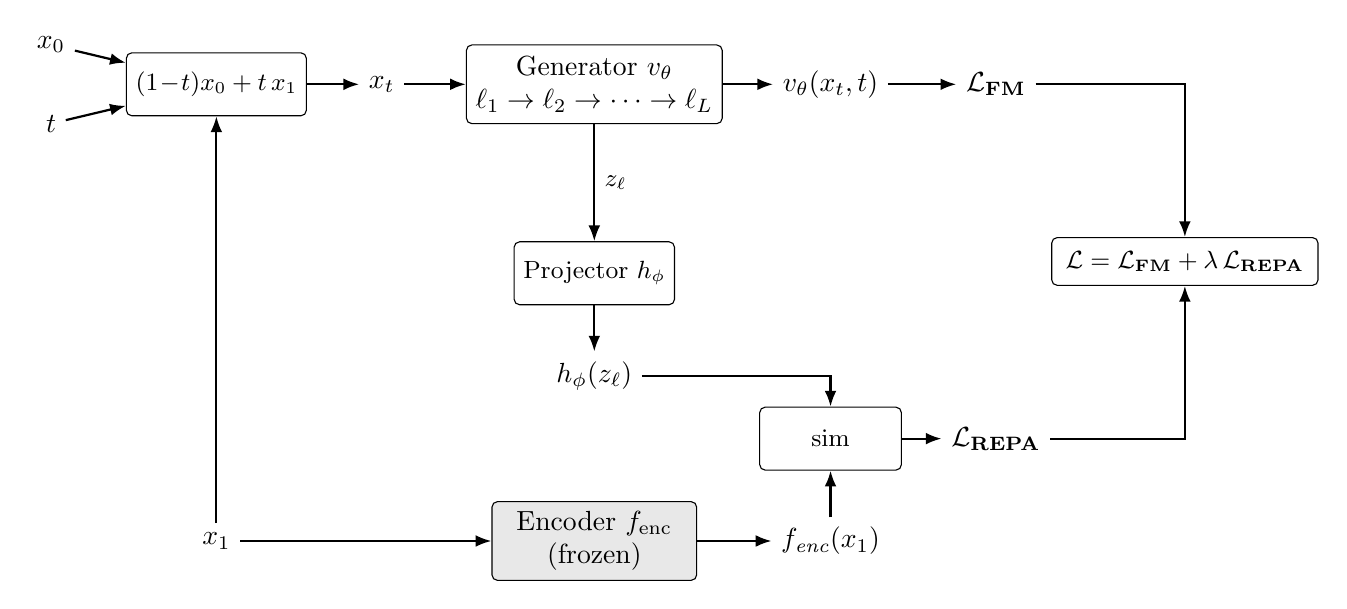
\begin{tikzpicture}[
    >={Latex[length=2mm]},
    block/.style={
        rectangle, draw, rounded corners=2pt,
        minimum height=10mm, minimum width=26mm,
        align=center
    },
    small/.style={
        rectangle, draw, rounded corners=2pt,
        minimum height=8mm, minimum width=18mm,
        align=center, font=\small
    },
    frozen/.style={fill=gray!18},
    lbl/.style={font=\itshape, align=center},
    loss/.style={font=\bfseries, align=center},
    arr/.style={-{Latex[length=2mm]}, thick}
]
\node[lbl] (x0) at (-2.6, 0.5) {$x_0$};
\node[lbl] (tinput) at (-2.6, -0.5) {$t$};
\node[small] (interp) at (-0.5, 0) {$(1\!-\!t)x_0 + t\,x_1$};
\node[lbl] (xt) at (1.6, 0) {$x_t$};
\node[block] (vtheta) at (4.3, 0) {Generator $v_\theta$ \\ $\ell_1 \to \ell_2 \to \cdots \to \ell_L$};
\node[lbl] (vout) at (7.3, 0) {$v_\theta(x_t,t)$};
\node[loss] (lfm) at (9.4, 0) {$\mathcal{L}_{\text{FM}}$};
\node[small] (proj) at (4.3, -2.4) {Projector $h_\phi$};
\node[lbl] (pemb) at (4.3, -3.7) {$h_\phi(z_\ell)$};
\node[lbl] (x1bot) at (-0.5, -5.8) {$x_1$};
\node[block, frozen] (fenc) at (4.3, -5.8) {Encoder $f_{\text{enc}}$ \\ (frozen)};
\node[lbl] (temb) at (7.3, -5.8) {$f_{\text{enc}}(x_1)$};
\node[small] (cos) at (7.3, -4.5) {sim};
\node[loss] (lrepa) at (9.4, -4.5) {$\mathcal{L}_{\text{REPA}}$};
\node[draw, rounded corners=2pt, inner sep=5pt, font=\small\bfseries, align=center]
  (ltotal) at (11.8, -2.25) {$\mathcal{L} = \mathcal{L}_{\text{FM}} + \lambda\, \mathcal{L}_{\text{REPA}}$};
\draw[arr] (x0) -- (interp);
\draw[arr] (tinput) -- (interp);
\draw[arr] (x1bot) -- (interp);
\draw[arr] (interp) -- (xt);
\draw[arr] (xt) -- (vtheta);
\draw[arr] (vtheta) -- (vout);
\draw[arr] (vout) -- (lfm);
\draw[arr] (vtheta) -- (proj) node[midway, right] {\small $z_\ell$};
\draw[arr] (proj) -- (pemb);
\draw[arr] (pemb) -| (cos);
\draw[arr] (x1bot) -- (fenc);
\draw[arr] (fenc) -- (temb);
\draw[arr] (temb) -- (cos);
\draw[arr] (cos) -- (lrepa);
\draw[arr] (lfm) -| (ltotal);
\draw[arr] (lrepa) -| (ltotal);
\end{tikzpicture}
\caption{The REPA construction. A noised sample $x_t = (1-t)x_0 + t\,x_1$ is constructed at each training step from a noise sample $x_0$, a clean data sample $x_1$, and a sampled timestep $t \in [0,1]$. The generator $v_\theta$ processes $x_t$ through its sequence of layers $\ell_1, \ldots, \ell_L$ to produce the velocity field that feeds the flow-matching loss $\mathcal{L}_{\text{FM}}$. Separately, the clean sample $x_1$ is also passed through a frozen pretrained encoder $f_{\text{enc}}$ (shaded). The generator's hidden state $z_\ell$ at the chosen alignment layer is mapped into the encoder's feature space by a trainable projector $h_\phi$; the REPA loss $\mathcal{L}_{\text{REPA}}$ is the negated similarity between $h_\phi(z_\ell)$ and $f_{\text{enc}}(x_1)$, averaged across tokens. The total training loss $\mathcal{L}$ combines them with weight $\lambda$.}
\label{fig:repa-construction}
\end{figure}

Chapter~\ref{ch:intro} introduced the argument made by Yu et al.~\cite{REPA} about the \emph{representation bottleneck} in diffusion-transformer models. It applies to flow-matching models too, by the equivalence above (\S\ref{sec:flow-matching}). The flow-matching objective implicitly asks a model to learn two things at once: a useful representation of the data, and a velocity field that interprets this representation. This twin burden, they argue, leads to slow convergence and large training budgets.

Their proposed solution, Representation Alignment (REPA), addresses the first half of this burden by adding a regularisation term to the training loss. Figure~\ref{fig:repa-construction} shows the construction. The regularisation pulls $z_\ell$, the generator's intermediate hidden state at a chosen \emph{alignment layer} $\ell$, towards the embeddings produced by a frozen pretrained encoder $f_{\text{enc}}$ run on the clean data sample $x_1$. The hidden state $z_\ell$ is a sequence of $N$ token vectors. In the context of images, each token represents an image patch; in the molecular setting, each token represents an atom or residue that is part of the larger molecule (\S\ref{sec:primer}). A small trainable \emph{projector head} $h_\phi$ --- a three-layer multi-layer perceptron (MLP) in the original paper --- maps $z_\ell$ into the encoder's feature space, so that $h_\phi(z_\ell)$ and $f_{\text{enc}}(x_1)$ can be compared. This alignment is asymmetric. The encoder provides a fixed target throughout training, while the generator parameters $\theta$ and the projector $\phi$ are updated.

The alignment loss is the negated similarity, averaged token-wise, between projected and target embeddings:
\[
  \mathcal{L}_{\text{REPA}} \,=\, -\, \mathbb{E}_{t,\, x_0,\, x_1} \left[ \frac{1}{N} \sum_{n=1}^{N} \operatorname{sim}\bigl( h_\phi(z_\ell)_n,\, f_{\text{enc}}(x_1)_n \bigr) \right],
\]
where $n$ indexes the $N$ tokens within a sample. In images $N$ is constant, so a token-wise average matches a per-sample-then-batch average; for molecules $N$ varies per sample, and the two diverge.

The final training objective is the flow-matching loss from \S\ref{sec:flow-matching} plus this term, scaled by a weight $\lambda$:
\[
  \mathcal{L} \,=\, \mathcal{L}_{\text{FM}} \,+\, \lambda\, \mathcal{L}_{\text{REPA}}.
\]

This construction exposes several design choices, some of whose effects we revisit in the ablations of Chapter~\ref{ch:proteina-study}:
\begin{itemize}
  \item The encoder $f_{\text{enc}}$, since different encoders capture distinct aspects of the data.
  \item The alignment layer $\ell$ at which the projector attaches. Yu et al.\ found mid-network layers best for images, but this is only an empirical observation.
  \item The alignment-loss weight $\lambda$, which balances alignment against the generative objective. Yu et al.\ used $0.5$ for images.
  \item The similarity metric $\operatorname{sim}$. We adopt cosine similarity, which Yu et al.\ found more effective than mean-squared error.
  \item The averaging mode. Averaging within each sample weights every molecule equally, while pooling across the batch gives larger molecules proportionally more REPA signal.
\end{itemize}

We adopt the core REPA construction as in Yu et al.\ for this report. However, a small family of methodological variants on REPA has since emerged. Dispersive regularisers~\cite{DiffuseDisperse} replace the external encoder with an internal contrastive term, while flexible-target formulations~\cite{REED} broaden which encoder features the loss attaches to. Separately, REPA-style alignment has been applied beyond the image setting, to video~\cite{VideoREPA}, audio~\cite{TARO}, materials~\cite{CrystalREPA}, and molecules~\cite{BoltzREPA}. We defer exploration of these variants to future work.

\subsection{What makes for a good REPA encoder?}
\label{sec:encoder-characterisation}


The encoder $f_{\text{enc}}$ is among REPA's largest design choices, but what makes a good alignment target? Yu et al.~\cite{REPA} observed that ImageNet linear-probe accuracy correlates positively with generation performance, suggesting global semantic representation is the driving factor. More recent work by Singh et al.~\cite{SpatialStructure} reports the opposite after profiling a wider range of encoders: linear-probe accuracy does not predict REPA gain, while a measure of the spatial structure of patch-token representations does. Generation performance may therefore be driven by \emph{local} feature geometry rather than \emph{global} semantic strength. Encoder characterisation for REPA remains open, particularly in the molecular setting, and we pick up the thread in Chapter~\ref{ch:profiling}.


\section{A primer on molecular generation}
\label{sec:primer}

\begin{figure}[!ht]
\centering
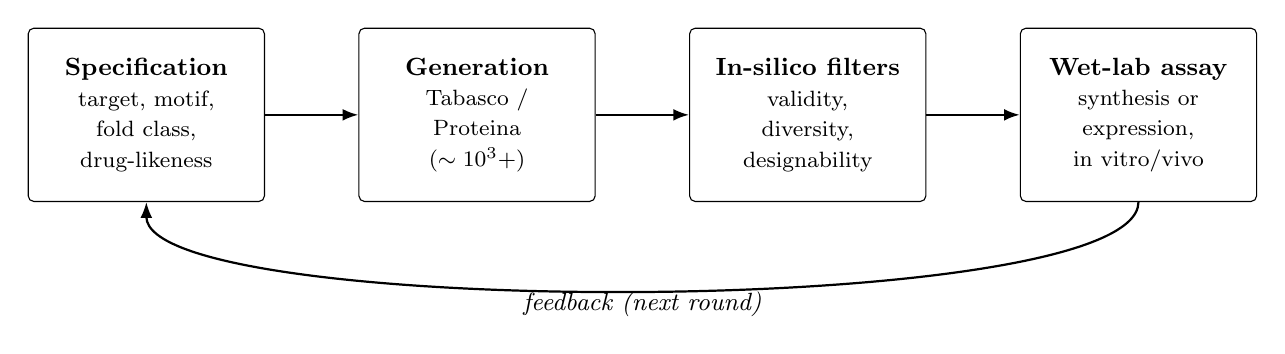
\begin{tikzpicture}[
    >={Latex[length=2mm]},
    block/.style={
        rectangle, draw, rounded corners=2pt,
        minimum height=22mm, minimum width=30mm,
        align=center, font=\small
    },
    lbl/.style={font=\itshape\small, align=center},
    arr/.style={-{Latex[length=2mm]}, thick}
]
\node[block] (spec) at (0, 0) {\textbf{Specification}\\\footnotesize{target, motif,}\\\footnotesize{fold class,}\\\footnotesize{drug-likeness}};
\node[block] (gen) at (4.2, 0) {\textbf{Generation}\\\footnotesize{Tabasco /}\\\footnotesize{Proteina}\\\footnotesize{($\sim 10^3$+)}};
\node[block] (filt) at (8.4, 0) {\textbf{In-silico filters}\\\footnotesize{validity,}\\\footnotesize{diversity,}\\\footnotesize{designability}};
\node[block] (lab) at (12.6, 0) {\textbf{Wet-lab assay}\\\footnotesize{synthesis or}\\\footnotesize{expression,}\\\footnotesize{in vitro/vivo}};
\draw[arr] (spec) -- (gen);
\draw[arr] (gen) -- (filt);
\draw[arr] (filt) -- (lab);
\draw[arr] (lab.south) .. controls (12.6, -2.6) and (0, -2.6) .. (spec.south);
\node[lbl] at (6.3, -2.4) {feedback (next round)};
\end{tikzpicture}
\caption{The de-novo molecular design cycle. An upstream specification drives a generative model to produce a candidate pool, which is funnelled through in-silico filters and then synthesised (or expressed) and assayed in the wet lab. Experimental results feed back into the next round of generation. Typical generation-step pool sizes are in the thousands to tens of thousands of candidates per round~\cite{RFdiffusion}.}
\label{fig:design-cycle}
\end{figure}

We now turn to the molecular setting, and the role generative models play within the broader de-novo molecular design pipeline. In a real-world scenario, generative models are rarely intended to produce ready-to-use artefacts. Instead, they act as high-throughput in-silico proposal engines in an iterative process of refinement and selection. This process, often called a \emph{design campaign}~\cite{Schneider2018}, is summarised in Figure~\ref{fig:design-cycle}.

An upstream specification, such as a drug-likeness profile or a fold class, conditions a generative model to produce a pool of candidate samples, which are then funnelled through in-silico filters. For small molecules, these typically include checks for structural validity and physical plausibility~\cite{PoseBusters}, drug-likeness~\cite{QED}, and target docking; for protein backbones, designability and structural diversity are the dominant considerations~\cite{Proteina}. The select few survivors are produced in a laboratory, through chemical synthesis (small molecules) or expression in cell lines (proteins), and evaluated using in-vitro or in-vivo assays. Experimental results then feed back into the next round of generation.

This pipeline framing is relevant to our discussion of evaluation metrics in Chapter~\ref{ch:evaluation}. Several metrics we adopt, such as structural validity and designability, are not measures of intrinsic molecular quality, but proxies for specific in-silico filter steps.

\section{Tabasco and Proteina}
\label{sec:molecular-domains}

The two models we study --- Tabasco~\cite{Tabasco} for small molecules and Proteina~\cite{Proteina} for protein backbones --- are both non-equivariant transformer flow-matching generators, designed to scale with data and model size rather than impose structural priors by construction.

Tabasco is motivated by the success of similar architectures in protein-structure generation, like Proteina, setting it apart from equivariant message-passing small-molecule generators such as EQGAT-diff~\cite{EQGATdiff}, MiDi~\cite{MiDi}, and SemlaFlow~\cite{SemlaFlow}. In turn, Proteina is motivated by the pair-bias attention mechanism introduced in AlphaFold~3~\cite{AlphaFold3}, which distinguishes it from SE(3)-equivariant backbone generators such as RFdiffusion~\cite{RFdiffusion}, FrameFlow~\cite{FrameFlow}, and Genie~\cite{Genie}. Despite their architectural minimalism, both achieve performance comparable or superior to equivariant baselines on quality evaluations.
\subsection{Small molecules and Tabasco}
\label{sec:small-mol}

In medicinal chemistry, a \emph{small molecule} is a drug-like compound at the sub-900-Dalton scale~\cite{NIHSmallMolGuide}. In-silico, its structure is typically represented using two coupled features: a discrete \emph{molecular graph} of typed atoms connected by typed bonds, and a continuous \emph{conformer} placing those atoms in 3D Cartesian space. A flow-matching model must therefore handle both parameterisations jointly.

Tabasco~\cite{Tabasco} represents each molecule as a sequence of per-atom tokens, each carrying an atom-type embedding and a 3D coordinate, but with no explicit bond decoder. This treats the molecule as a point cloud of typed atoms rather than a graph, sidestepping edge modelling at the cost of having to recover bond structure post hoc from interatomic distances. Tabasco is trained on GEOM-drugs~\cite{GEOMdrugs}, a public dataset of drug-like conformers.

This point-cloud-of-atoms parameterisation is one of several, each with a different trade-off. \emph{SMILES} and \emph{SELFIES} string encodings discard the 3D conformer entirely. \emph{3D voxel grids} preserve geometry but lose the graph and inflate the token count. \emph{Equivariant point clouds}, used by EQGAT-diff~\cite{EQGATdiff}, MiDi~\cite{MiDi}, and SemlaFlow~\cite{SemlaFlow}, keep both but require SE(3)-equivariant layers. See Duval et al.~\cite{HitchhikersGuide} and Wang et al.~\cite{MoleculeDiffusionSurvey} for broader surveys.
\subsection{Protein backbones and Proteina}
\label{sec:protein}

A \emph{protein} is a chain of amino-acid residues, ranging from around 50 to several thousands in length~\cite{BritannicaProtein}; the largest known, titin, has approximately 34,000 residues. (Shorter chains are typically classified as \emph{peptides} instead.) Each amino-acid residue contributes four \emph{backbone} atoms (N, C$_\alpha$, C, O) whose interactions determine the chain's \emph{fold} geometry, and a \emph{side chain} that determines its amino-acid identity.

A protein's \emph{secondary structure} is its local pattern of $\alpha$-helices and $\beta$-strands; its \emph{tertiary structure} is the global three-dimensional fold those elements form when they pack together. A CATH code~\cite{CATH} (Class, Architecture, Topology, Homology) classifies this fold hierarchically. \emph{Class} captures broad secondary-structure content (mostly-$\alpha$, mostly-$\beta$, or mixed), \emph{Architecture} the gross spatial arrangement of those elements, and \emph{Topology} their specific connectivity.

For the structure-generation problem we study, it is customary to model only the backbone, with sequence identity recovered downstream by a separate \emph{inverse-folding} model such as ProteinMPNN~\cite{ProteinMPNN}. The \emph{CA-trace} compresses this further, using only the C$_\alpha$ coordinate of each residue. It retains enough information to recover fold topology, at lower cost than the fuller \emph{all-atom} representation. Proteina~\cite{Proteina} adopts this C$_\alpha$ parameterisation, representing each backbone as a sequence of per-residue tokens carrying continuous C$_\alpha$ Cartesian coordinates. The models reported in the original presentation are largely trained on high-confidence synthetic structures from the AlphaFold Database (AFDB)~\cite{AFDB}.

Again, the CA-trace is one of several protein parameterisations. \emph{Sequence-only} models such as the ESM lineage~\cite{ESM2} operate on amino-acid strings, capturing rich functional priors but little 3D structure. \emph{Full-atom} representations close the gap to physical realism at substantial compute cost. \emph{Equivariant} parameterisations, such as torsion angles and oriented residue frames, encode SE(3) symmetries by construction and underlie the equivariant generators noted above, but have historically bottlenecked scaling. See Notin et al.~\cite{NotinProteinDesign} for a broader survey.

\section{Open questions}
\label{sec:open-questions}


This survey leaves open the two questions of \S\ref{sec:contributions}. First, \emph{does REPA work for molecules?} Existing molecular REPA work~\cite{REED,BoltzREPA} has not ablated over encoder choice, and protein backbone generation in particular remains unexplored. Second, \emph{when does REPA work?} The encoder-characterisation work introduced in \S\ref{sec:encoder-characterisation} has begun to ask which encoder properties predict REPA gain, but only for images, and we seek to explore this further. We take up both questions in Chapters~\ref{ch:profiling}--\ref{ch:proteina-study}.

\chapter{Evaluating molecular generation}
\label{ch:evaluation}



\emph{What does it mean for a model to generate ``good'' artefacts?} In this chapter, we outline a framework for evaluating molecular generation, and the tensions inherent to this endeavour. We argue that no single number suffices here, define the metric suites we use for small molecules (Table~\ref{tab:eval-smallmol}) and protein backbones (Table~\ref{tab:eval-protein}), and introduce the probe principle by which we measure a model's internal representations. We also introduce the theme of a \emph{trade-off frontier} with these metrics. A gain on one axis may imply a loss on another (Chapter~\ref{ch:proteina-study}), so finding an acceptable balance, or better yet, pushing this envelope, is very useful.

\section{What makes for a ``good'' molecule?}
\label{sec:eval-good}

``Goodness'' is usually task-specific, and a de-novo design pipeline (\S\ref{sec:primer}) asks several things of a generated candidate pool at once. A useful set must at least be \emph{valid}: realistic enough to survive downstream filters; \emph{diverse}: spread across the design space, not collapsed onto a few modes; and \emph{designable}: amenable to synthesis. These axes trade off against each other. A model can buy validity by memorising a handful of safe scaffolds, at the cost of diversity; or buy diversity by spreading its mass thinly, at the cost of designability. No axis is dispensable, and maximising any one in isolation is uninformative, as these metrics are themselves proxies for the pipeline's real-world filter steps.

\section{Representation and generation are multi-factorial and multi-scale problems}
\label{sec:eval-multifactorial}


Moreover, the need for a suite of evaluation metrics reflects how molecules are represented in-silico. Molecules present a stark contrast with images, which originated the generative machine learning methods we adopt (\S\ref{sec:flow-matching}).

In a 2D image, \emph{geometry} and \emph{content} are coupled in one representation. The pixel grid is at once an object's shape and its identity. There is a single contiguous feature space, so one self-supervised encoder can serve as a near-complete description of it. This coupling is what lets image generation lean on a single strong encoder, and lets image quality be summarised, to a first approximation, by a single Fr\'echet distance in that encoder's feature space~\cite{FID}.

However, molecules pull geometry and content apart, and into more than two pieces. A molecule is at once a discrete graph of typed atoms drawn from a periodic-table-sized alphabet, and a continuous 3D geometry. This is a discrete--continuous duality with no clean analogue in the pixel grid. The two concepts are only loosely tied: one bonding graph admits many conformers, and similar geometries can host different atom types. Geometry is itself organised hierarchically from local environments up to global shape. Indeed, the taxonomy used to describe protein structure makes this explicit, running from primary sequence through secondary-structure elements to the tertiary fold.

As a consequence, both representation and generation quality are \emph{multi-factorial} and \emph{multi-scale} in this domain. No single encoder captures every factor of content and geometry at every scale at once, as we see in Chapter~\ref{ch:profiling}. Moreover, no single metric can score a generated set along all those factors at once. A model can match the distribution of folds while getting local geometry subtly wrong; it can place atoms in valid positions while collapsing the diversity of shapes it produces. These are independent failures, so mode collapse is harder to reason about than in the image domain, where one number suffices to track what goes wrong.

The metric suite we propose in this chapter is an attempt at handling this complexity. We decompose quality along the factors the domain pulls apart, and interpret metrics holistically to understand the complete picture. For each domain we report two complementary families: \emph{representation quality}, which scores what the model encodes internally, and \emph{generation quality}, which scores its outputs. We present them in that order throughout the report, since representation is what REPA's mechanism acts on (\S\ref{sec:repa}) and generation is the outcome we hope it improves.

\section{The linear probe principle}
\label{sec:eval-probe}

One way to understand what a model represents internally is the \emph{linear probe}. We freeze the model, extract its hidden states for clean inputs, and fit a linear regression to a known structural label. If the label is recoverable by this simple probe, that information is considered to be present and accessible in the representation; if not, it is considered absent or deeply entangled. This follows standard practice in image generation, where encoders are often characterised by ImageNet linear-probe accuracy~\cite{REPA}. We use this mechanism in two places: on the frozen encoders we might align to (Chapter~\ref{ch:profiling}), and on the generator trunk itself (Chapters~\ref{ch:tabasco-study} and~\ref{ch:proteina-study}).

The form of the read-out follows the label. For real-valued targets, we fit a regression and score recoverability by held-out $R^2$. For categorical targets, we fit a logistic classifier and score top-1 accuracy.

We outline the small-molecule targets we regress against in \S\ref{sec:eval-small-mol}, and the protein suite in \S\ref{sec:eval-protein}. Each probe maps to a necessary condition for a useful alignment target. The tasks span content and geometry from local to global scales, so we interpret a representation that scores well across the whole battery as genuinely carrying holistic information.

\section{Small-molecule metrics}
\label{sec:eval-small-mol}

Table~\ref{tab:eval-smallmol} collects every small-molecule metric we use, following the conventions of recent 3D molecular generators~\cite{Tabasco,EQGATdiff,SemlaFlow}.

\textbf{Representation quality.} This asks what structural information the generator has learned to encode internally. We apply the probe principle of \S\ref{sec:eval-probe}, regressing mean-pooled per-atom features onto four global RDKit descriptors~\cite{RDKit} --- molecular weight, LogP, ring count, and rotatable-bond count --- and score recoverability by held-out $R^2$.

\textbf{Generation quality.} This asks if the generator produces good artefacts. For small molecules, quality metrics fall into three groups: per-molecule \emph{structural quality} (validity, connectivity, uniqueness), set-level \emph{coverage} (diversity, novelty), and \emph{distributional realism} (the Fr\'echet ChemNet Distance, FCD~\cite{FCD}). The first group guards against malformed or repeated molecules; the second against mode collapse and memorisation; FCD, the small-molecule analogue of the image-domain Fr\'echet Inception Distance~\cite{FID}, asks whether the generated set as a whole resembles real molecules. As we explore in Chapter~\ref{ch:tabasco-study}, the structural-quality metrics are particularly amenable to saturation by a strong generator. This does not mean the problem is solved; rather, it is a limit of the yardstick itself.

% Ch3 eval table -- ALL small-molecule metrics (representation + generation). \input{} from report-draft.tex Ch3.
\begin{table}[tbp]
\centering
\small
\setlength{\tabcolsep}{5pt}
\begin{tabular}{l >{\raggedright\arraybackslash}p{0.44\textwidth} >{\raggedright\arraybackslash}p{0.18\textwidth} l}
\toprule
\textbf{Metric} & \textbf{Definition} & \textbf{Captures} & \textbf{Score} \\
\midrule
\multicolumn{4}{l}{\textbf{Representation quality} --- probe recoverability of RDKit descriptors~\cite{RDKit}} \\
MolWt\,$\uparrow$    & Molecular weight & Global size & $R^2$ \\
LogP\,$\uparrow$     & Octanol--water partition coefficient & Lipophilicity & $R^2$ \\
Rings\,$\uparrow$    & Ring count & Topology & $R^2$ \\
RotBonds\,$\uparrow$ & Rotatable-bond count & Flexibility & $R^2$ \\
\midrule
\multicolumn{4}{l}{\textbf{Generation quality}} \\
\addlinespace
\multicolumn{4}{l}{\textit{Structural quality}} \\
Validity\,$\uparrow$     & Fraction sanitising to a valid molecule once bonds are inferred & Malformed geometry & Fraction \\
Connectivity\,$\uparrow$ & Fraction forming a single connected component & Fragmentation & Fraction \\
Uniqueness\,$\uparrow$   & Fraction not duplicating another generation & Trivial repetition & Fraction \\
\addlinespace
\multicolumn{4}{l}{\textit{Set coverage}} \\
Diversity\,$\uparrow$ & Mean pairwise dissimilarity across the set & Mode collapse & Fraction \\
Novelty\,$\uparrow$   & Fraction of the set absent from the training data & Memorisation & Fraction \\
\addlinespace
\multicolumn{4}{l}{\textit{Distributional realism}} \\
FCD\,$\downarrow$~\cite{FCD} & Fr\'echet ChemNet Distance: Fr\'echet distance to a reference set in a property-prediction network's feature space & Distribution mismatch & Distance \\
\bottomrule
\end{tabular}
\caption{Small-molecule metrics (Chapter~\ref{ch:tabasco-study}), following the conventions of
recent 3D molecular generators~\cite{Tabasco,EQGATdiff,SemlaFlow}. Representation quality is
probe recoverability of global RDKit descriptors (held-out $R^2$); generation quality spans
per-molecule structural quality, set-level coverage, and distributional realism. Arrows give
the good direction. The structural-quality metrics are bounded above and saturate against a
strong baseline; FCD is the one generation axis with no hard ceiling.}
\label{tab:eval-smallmol}
\end{table}


\section{Protein-backbone metrics}
\label{sec:eval-protein}

Protein backbones are larger and more variable than small molecules (Chapter~\ref{ch:background}), and evaluating them is correspondingly more involved. Table~\ref{tab:eval-protein} collects all the protein metrics we use. We present representation first, then generation, and close by offering our own framework for how the generation metrics should be grouped and read together.

% Ch3 eval table -- ALL protein-backbone metrics (representation quality + alignment + generation). \input{} from report-draft.tex Ch3.
\begin{table}[tbp]
\centering
\small
\setlength{\tabcolsep}{4pt}
\begin{tabular}{l >{\raggedright\arraybackslash}p{0.38\textwidth} >{\raggedright\arraybackslash}p{0.20\textwidth} l}
\toprule
\textbf{Metric} & \textbf{Definition} & \textbf{Content} & \textbf{Granularity} \\
\midrule
\multicolumn{4}{l}{\textbf{Representation quality}} \\
IF top-1\,$\uparrow$       & Inverse-folding sequence recovery (top-1 accuracy)~\cite{Ingraham2019} & Local chemical env. & Per residue \\
Dihedral MAE\,$\downarrow$ & Backbone dihedral-angle error~\cite{ProteinWorkshop} & Low-level geometry & Per residue \\
CATH-A top-1\,$\uparrow$   & Fold-architecture classification top-1 accuracy~\cite{ProteinWorkshop} (Table~\ref{tab:setup-cath}) & Global fold & Per chain \\
\midrule
\multicolumn{4}{l}{\textbf{Representation alignment}} \\
CKNNA\,$\uparrow$~\cite{PlatonicRep} & Mutual-nearest-neighbour kernel alignment & Trunk--encoder similarity & Per residue \\
\midrule
\multicolumn{4}{l}{\textbf{Generation quality}} \\
\addlinespace
\multicolumn{4}{l}{\textit{Quality}} \\
FPSD\,$\downarrow$          & Fr\'echet Protein Structure Distance: distance to the reference set in a structural encoder's (GearNet) feature space & Distributional fidelity & Whole set \\
Des\,$\uparrow$            & Fraction of samples that are designable & Physical realisability & Whole set \\
\addlinespace
\multicolumn{4}{l}{\textit{Tertiary structure --- whole set (T-W)}} \\
fJSD-A\,$\downarrow$       & Jensen--Shannon divergence vs.\ reference CATH-A distribution & Fold-distribution fidelity & Whole set \\
fS-A\,$\uparrow$           & Spread of generated folds across CATH-architecture classes & Whole-set fold diversity & Whole set \\
\addlinespace
\multicolumn{4}{l}{\textit{Tertiary structure --- designable subset (T-D)}} \\
\#Clust\,$\uparrow$        & Number of TM$\,\ge\,$0.5 structural clusters & Designable diversity & Designable subset \\
pwTM\,$\downarrow$         & Mean pairwise TM-score, designable subset & Designable diversity & Designable subset \\
\addlinespace
\multicolumn{4}{l}{\textit{Secondary structure --- whole set (S-W)}} \\
ssJSD-2D\,$\downarrow$     & Jensen--Shannon divergence of the (helix-frac, strand-frac) distribution & Secondary-structure fidelity & Whole set \\
\addlinespace
\multicolumn{4}{l}{\textit{Secondary structure --- designable subset (S-D)}} \\
ssJSD-2D\,$\downarrow$     & As above, on the designable subset & SS fidelity (designable) & Designable subset \\
E\%des\,$\uparrow$         & Mean $\beta$-strand (E) fraction & $\beta$-content & Designable subset \\
\bottomrule
\end{tabular}
\caption{Protein-backbone metrics (Chapter~\ref{ch:proteina-study}), across three measurement
families: representation quality (probe recoverability spanning local-to-global structure),
representation alignment (trunk-to-encoder similarity), and generation quality (the five
reported groups). The whole set is all generated backbones; the designable subset is those
passing the designability filter. Arrows give the good direction. Full per-metric results
appear in Tables~\ref{tab:proteina-700k} and~\ref{tab:proteina-concentration}.}
\label{tab:eval-protein}
\end{table}


\textbf{Representation quality.} We apply the probe principle of \S\ref{sec:eval-probe} for three tasks adapted from the literature, spanning local to global structure: per-residue inverse-folding recovery~\cite{Ingraham2019} for the local chemical environment; backbone dihedral error~\cite{ProteinWorkshop} for low-level geometry; and CATH fold classification~\cite{ProteinWorkshop} for global fold. The first two are scored per residue (top-1 accuracy and mean absolute error), while the fold probe is a logistic classifier on mean-pooled per-chain features. Because the three are largely orthogonal, improving all of them at once is strong evidence of holistic representation quality.

\textbf{Representation alignment.} This asks not what the generator encodes, but how geometrically close it sits to a frozen encoder. We measure it with CKNNA~\cite{PlatonicRep}, a mutual-nearest-neighbour kernel alignment, following the original REPA analysis~\cite{REPA} and a recent molecular extension~\cite{BoltzREPA}. We use it as a diagnostic lens on how REPA acts rather than a quantity we optimise.

\textbf{Generation quality.} Measures of generation quality draw on two lineages. The \emph{canonical} ones --- designability, and various counts of novelty and diversity --- score or tally individual generations, and predate modern generative models. The \emph{model-based} ones, introduced to this domain by Proteina~\cite{Proteina}, borrow the idea from image generation of comparing a generated set against a reference in a learned feature space. We headline on one from each: designability as the canonical measure of per-sample quality, and the Fr\'echet Protein Structure Distance (FPSD) as the model-based measure of set-level distributional realism. We outline these two metrics, add a secondary-structure metric of our own, and then set out a framework that organises them all.

\textbf{Designability.} This metric estimates the fraction of generated backbones that are realisable as real proteins. It involves an in-silico round-trip through the protein design loop (\S\ref{sec:protein}). Each backbone is inverse-folded with ProteinMPNN~\cite{ProteinMPNN}, a model trained to predict an amino-acid sequence that would fold into a given backbone, to propose candidate sequences. These sequences are then re-folded with ESMFold, a model trained to predict 3D structure from sequence. A backbone is termed designable when the self-consistency root-mean-squared deviation (scRMSD) between the generated backbone and its re-folded prediction falls below 2\,\AA{}.

One caveat affects interpretation: designability is an in-silico proxy, not ground-truth physical realism, so it inherits the biases of the folding models it relies on. The inverse-folding and folding steps share model lineage with AlphaFold2~\cite{AlphaFold2}, and hence with the synthetic AlphaFold Database (AFDB), whose structures are themselves AF2 predictions. Generators trained on AFDB therefore score systematically higher on designability by construction, as we explore in Chapter~\ref{ch:proteina-study}.

\textbf{Designable $\beta$-strand \%.} A model can inflate designability by emitting easy, highly foldable all-$\alpha$ backbones, since idealised helical bundles re-fold with low scRMSD almost by construction. On the contrary, $\beta$-strand content is harder to render designable. As a guard-rail, we track the mean fraction of residues in $\beta$-strand ($f_E$) over the designable subset, and read it alongside designability. A designable set that retains $\beta$-rich folds is evidence that its designability is genuine, rather than bought with trivial helical artefacts. (We use the C$\alpha$-only secondary-structure assignment of Appendix~\ref{app:ssjsd}.)

\textbf{FPSD.} The Fr\'echet Protein Structure Distance~\cite{Proteina} is the protein analogue of the imaging FID. First, it embeds the generated and reference sets using an external encoder: in this case, a GearNet~\cite{GearNet} model trained on a fold classification task. Then, it models each set of embeddings as a Gaussian, and reports the Fr\'echet distance between the two --- a scalar that drops to zero as the generated distribution matches the reference in both mean and covariance. Because the encoder reads fold-level geometry, FPSD scores how well a generated set reproduces the reference distribution of folds. As a distributional distance, FPSD also rewards matching the spread of the reference, not just its centre. It therefore carries some diversity signal of its own, which is why it and our dedicated diversity metrics often move together. This GearNet fold classifier is also one of our two REPA alignment targets in our study of protein backbones (Chapter~\ref{ch:proteina-study}). A model aligned to it might then be expected to gain on FPSD mechanically, by being pulled toward the metric's own feature space. We check this in \S\ref{sec:proteina-convergence} and find it does not hold.

\textbf{ssJSD-2D.} We introduce this secondary-structure metric in our report. Like FPSD and fJSD, it is a \emph{distributional} metric, scoring the generated secondary-structure distribution against a real reference. Proteina already measures this, but only at the level of mean helix and strand content, which is blind to a model that matches the average composition while collapsing its spread. In contrast, ssJSD-2D is a Jensen--Shannon divergence over the full joint (helix-fraction, strand-fraction) distribution against the reference, so it rewards reproducing the whole spread of secondary-structure content, not just its centre. The per-residue helix, strand, and coil labels come from the P-SEA algorithm~\cite{PSEA}, run on C$\alpha$ coordinates alone, as implemented in Biotite~\cite{Biotite} (Appendix~\ref{app:ssjsd}).

\textbf{A two-axis taxonomy.} We propose reading all these metrics through a framework that organises them by structural and distributional relevance. Two axes do the work: \emph{tertiary} versus \emph{secondary} structure, and the \emph{whole set} versus the \emph{designable subset}. The result is a grid of metric groups, which the result tables in Chapter~\ref{ch:proteina-study} lay out as supercolumns. \emph{Tertiary-whole (T-W)} asks whether the distribution of global folds matches a reference over all backbones; its flagship is FPSD, alongside fJSD (a Jensen--Shannon divergence between the generated and reference fold-class distributions) and a fold-spread score (fS)~\cite{Proteina}. Both fJSD and fS are defined at each level of the CATH hierarchy (\S\ref{sec:protein}); we headline on the architecture level (fJSD-A, fS-A). \emph{Tertiary-designable (T-D)} asks the same diversity question, but only of backbones that pass designability. Its canonical measure in the protein-backbone literature is the cluster count, the number of distinct structural clusters the designable set falls into~\cite{Proteina}. That count is sensitive to the number of designable backbones, however, which varies across our models --- a model that simply passes more backbones forms more clusters without being any more diverse. We therefore use the pairwise TM-score (pwTM) throughout instead. As a pairwise average, pwTM stays robust at the small sizes of the designable subset, where a distributional measure like fS is unreliable. \emph{Secondary-whole (S-W)} and \emph{secondary-designable (S-D)} apply ssJSD-2D over the same two populations.

\textbf{A caveat on noise.} We also note that generative metrics are noisy, so a gap between two point estimates is not necessarily a finding. We report bootstrap intervals and seed sweeps where possible to guard against this.

\section{The designability--diversity trade-off}
\label{sec:protein-tradeoffs}

A central dynamic in protein generation pits the designability number against the diversity of the designable subset (T-D). A model can trivially raise its designability number by collapsing onto a few reliable, highly foldable modes, but this shrinks the diversity of that designable subset. Pushing designability up therefore tends to push designable-subset diversity down, and vice versa. This dynamic is noted regularly in the literature~\cite{Proteina}, and is typically modulated by a choice of sampler noise.

Ultimately, how does this trade-off help us compare models? In our studies, we distinguish between two phenomena. The first is whether a model merely occupies a different spot on the same envelope, in which case the optimal choice is use-case specific. The second is whether a model pushes the envelope itself --- playing the same trade-off game, but at a higher level, winning on one axis without conceding the other. This makes a model canonically better.

These complex dynamics further motivate the question: \emph{what makes an encoder a good teacher of representational information in this domain?} We examine this question in Chapter~\ref{ch:profiling}, which informs the experiments we present in Chapters~\ref{ch:tabasco-study} and ~\ref{ch:proteina-study}.

\chapter{Encoder targets and profiling}
\label{ch:profiling}


\emph{What properties make an encoder a good target for representation alignment?} This question is unsettled in the image domain, with global semantic quality and local spatial structure both proposed as the driver (\S\ref{sec:encoder-characterisation}).

In this chapter, we ask this question in the molecular domain. Earlier, we discussed how molecular representation is multi-factorial and multi-scale (\S\ref{sec:eval-multifactorial}), which means that no single pre-trained encoder is likely to capture all of it. An encoder is typically optimised for one task in isolation, and sees a molecule through that lens. For example, an interatomic-potential model reads local geometry; a fold classifier reads global shape; a sequence model reads chemical identity. The encoder we align to therefore selects which factor REPA is most likely to transfer.

Our profiling work in this chapter makes this concrete. We build a suite of diagnostics to assess what information an encoder contains, how much of it is relevant to the generative task, and how well conditioned its embeddings are. We use this to profile seven candidate encoders across small molecules and proteins, and then use the results to guide which encoders to align with in the studies of Chapters~\ref{ch:tabasco-study} and~\ref{ch:proteina-study}.

\section{A profiling protocol}
\label{sec:profiling-framework}

We profile every candidate encoder with the protocol summarised in Table~\ref{tab:profiling-diagnostics}. Each encoder is run frozen on a sample of structures from our training sets: 200--2{,}000 molecules (QM9 and GEOM) for the small molecule encoders, and 200 proteins (PDB) for the protein encoders. This yields one embedding vector per atom or residue --- tens of thousands of vectors in each case --- and every diagnostic is computed from these per-token embeddings.

% Ch4 profiling-diagnostics table. \input{} from sec:profiling-framework.
% Grouped by the three properties (information / recoverability / conditioning), with the
% upper-bound / lower-bound framing carried in the group glosses.
\begin{table}[tbp]
\centering
\small
\setlength{\tabcolsep}{4pt}
\begin{tabular}{l >{\raggedright\arraybackslash}p{0.28\textwidth} >{\raggedright\arraybackslash}p{0.42\textwidth}}
\toprule
\textbf{Diagnostic} & \textbf{What it captures} & \textbf{How we compute it} \\
\midrule
\multicolumn{3}{l}{\textbf{Information}\quad\textit{what the encoder encodes --- an upper bound on what REPA can transfer}} \\
3D geometry          & sensitivity to 3D pose                & cosine similarity after a small coordinate perturbation \\
Token identity       & atom or residue type                  & linear-probe accuracy \\
Object identity      & tokens of the same molecule or protein & within- minus between-object cosine similarity \\
Secondary structure  & helix, sheet, or loop (proteins)      & within- minus between-SS cosine similarity \\
\addlinespace
\multicolumn{3}{l}{\textbf{Recoverability}\quad\textit{what a projector recovers from cheap inputs --- a lower bound}} \\
Cheap-input ladder   & constant $\to$ identity $\to$ identity${+}$position & cosine similarity a same-form MLP reaches at each rung \\
\addlinespace
\multicolumn{3}{l}{\textbf{Conditioning}\quad\textit{whether the embedding is well-formed}} \\
Effective rank       & dimensions actually used              & RankMe (Roy--Vetterli effective rank) \\
Sparsity, dead dims  & degenerate dimensions                 & fraction of exact zeros; permanently inactive dimensions \\
Norm scale           & numerical conditioning                & mean embedding $\ell_2$ norm \\
\bottomrule
\end{tabular}
\caption{The profiling diagnostics, grouped by the three properties of Figure~\ref{fig:profiling-framework}.}
\label{tab:profiling-diagnostics}
\end{table}


We ask three things of each encoder, and a good target needs all three.

\textbf{Information} asks: \emph{what does the encoder contain?} This estimates the upper bound on what REPA can add to a model. Alignment cannot teach anything the encoder does not itself hold. For a 3D generator, the axis that matters most is 3D geometry. We measure geometry-awareness by how far the embedding moves under a change in 3D pose: across distinct conformers of the same molecule for the molecular encoders, and after a 1\,\AA{} coordinate perturbation for the protein encoders, where only a single structure is available. We also report token identity, since a high score there suggests that an encoder is performing an identity lookup that the generator may already be capable of.

\textbf{Relevance} asks: \emph{how much of a REPA target can the generator match without improving the representation it is trying to learn?} A generator does not need to learn all the information contained in an encoder. Indeed, during training, it is fed most of the relevant \emph{content} of the molecule directly: the normalised token index always, and, for molecules, a one-hot of the atom type (the protein generator is given position but not residue identity; see \S\ref{sec:profiling-protein}). What it must acquire is the 3D \emph{geometry}, which it sees only as noisy coordinates it is being trained to denoise. Hence, a REPA target is relevant only insofar as matching it forces the generator to improve that geometric representation.

A target can fail this in two ways:
\begin{itemize}[topsep=2pt,itemsep=1pt]
  \item \emph{cheatable}: the target is trivially reconstructible from inputs the generator already holds. So the model can saturate alignment loss without actually learning a better representation.
  \item \emph{off-task}: matching the target does require representation learning, but what it requires is not what we need. For example, since the protein generator is not given residue identity, matching an identity-encoding target would force it to infer sequence from backbone. This is a genuine learning problem, but a different one from generating geometry, so the pressure may not assist the task we care about.
\end{itemize}

We estimate the cheatable fraction directly. We fit a three-layer MLP, the same projector that REPA uses (\S\ref{sec:repa}), to reconstruct embeddings from cheap features that withhold all 3D geometry: first \emph{identity} alone (a one-hot of the atom or residue type), then \emph{identity${+}$position} (Table~\ref{tab:profiling-diagnostics}). Separately, with no projector fit, we also score the \emph{constant} dataset mean, which is the optimal input-free prediction. We read this constant baseline as the \emph{floor}, and the rise of the fitted rungs above it as the \emph{lift}.

Read together, the floor and lift sort an encoder into one of three configurations:
\begin{itemize}[topsep=2pt,itemsep=1pt]
  \item high floor suggests \emph{saturation}. The embeddings barely vary, so a constant prediction already matches them. There is little signal to align to.
  \item low floor, high lift suggests \emph{cheatable}. The embeddings vary, but the cheap inputs reconstruct that variation, so it is largely an identity lookup using data the generator is already fed.
  \item low floor, low lift is \emph{promising}. However, a low lift only says the variation does not stem from the cheap identity we tested. It does not positively affirm that it comes from the geometry a generator needs. We interpret this against the information probes to tell a geometric encoder from one varying for some \emph{off-task} reason.
\end{itemize}

\textbf{Conditioning} asks: \emph{is the embedding mathematically well-formed enough to be a target?} For example, an embedding whose variance has collapsed onto a few directions (a low effective rank), or that is mostly zero, is a bottleneck. Too little structure passes through for the alignment to transmit anything, no matter the information or the relevance.

We apply this protocol to molecule encoders first (\S\ref{sec:profiling-mol}), then protein encoders (\S\ref{sec:profiling-protein}), and draw together what it implies in \S\ref{sec:profiling-predictions}.

\section{Small molecule encoders}
\label{sec:profiling-mol}

% Molecule encoder-zoo profiling table. \input{} from report-draft.tex Ch4 (sec:profiling-mol).
% Numbers from encoder_profiling/tabasco/FINDINGS.md. CheMeleon RankMe re-run 2026-06-04 (rdkit-env fix):
% QM9 1194.7 / GEOM 1165.6 out of 2048; now the same metric as MACE (Roy--Vetterli effective rank on
% raw sigma), so directly comparable. GEOM value shown (Ch5 trains on GEOM-drugs).
% Floor = mean-direction cosine; Lift = best-projector minus floor (the old "Gap" column).
\begin{table}[tbp]
\centering
\small
\setlength{\tabcolsep}{4pt}
\begin{tabular}{l r cc cc cc l}
\toprule
 & & \multicolumn{2}{c}{\textbf{Information}} & \multicolumn{2}{c}{\textbf{Relevance}} & \multicolumn{2}{c}{\textbf{Conditioning}} & \\
\cmidrule(lr){3-4}\cmidrule(lr){5-6}\cmidrule(lr){7-8}
\textbf{Encoder} & \textbf{Dim} & 3D & atom-$\Delta$ & Floor & Lift & Sparsity & RankMe & \textbf{Verdict} \\
\midrule
CheMeleon (2D graph)    & 2048 & no       & 0.093 & 0.43 & $+0.04$  & 93.8\% & 1166 & off-task \\
MACE (3D potential)     & 192  & weak     & 0.260 & 0.86 & $+0.005$ & 0\%    & 40.6 & saturated \\
\bottomrule
\end{tabular}
\caption{Molecule encoder profiles. \emph{3D-aware}: whether the embedding changes across conformers (CheMeleon is bit-identical, L2~$=0$; MACE shifts only slightly, cosine $0.995$). \emph{atom-$\Delta$}: same-element, different-environment cosine-similarity spread. \emph{Floor}: cosine similarity of a constant prediction (high $=$ saturated). \emph{Lift}: cosine similarity a same-form MLP gains above the floor from cheap inputs. \emph{Sparsity} and \emph{RankMe} (effective rank out of \emph{Dim}~\cite{RankMe}) measure conditioning. CheMeleon's lift is real but conformation-invariant 2D context, off-task for guiding 3D geometry; its high RankMe is a diffuse, sparse embedding that overflows the 128-dimensional projector input. MACE carries the right kind of signal, but a high floor leaves a lift of only $+0.005$.}
\label{tab:profiling-mol}
\end{table}


We profile two publicly available pre-trained encoders, summarised in Table~\ref{tab:profiling-mol} (full values in Appendix~\ref{app:profiling-full}). They bracket a useful contrast. One sees the 2D bonding graph, the other sees 3D geometry. Neither, the framework finds, is a clean alignment target.

CheMeleon~\cite{CheMeleon} is a directed message-passing network (a ChemProp D-MPNN) that passes messages along the bonds of the 2D molecular graph; it never sees coordinates. Its embeddings are well spread (a low floor), but it fails on two other counts. First, it is 93.8\% sparse, so alignment runs over a shifting, ill-conditioned subspace. Second, it is conformer-invariant by construction, so its lift is 2D bond-graph context, which may not aid a 3D generator.

MACE~\cite{MACE} is an equivariant message-passing network built on many-body atomic interactions, pretrained as an interatomic potential to predict energies from 3D structure. The model's embeddings are mathematically well-formed. However, its energy pretraining captures local environments over global pose, so its 3D signal is weak, and a high floor of 0.86 suggests it is mean-saturated.

\section{Protein backbone encoders}
\label{sec:profiling-protein}

% Protein encoder-zoo profiling table. \input{} from report-draft.tex Ch4 (sec:profiling-protein).
% Numbers from encoder_profiling/proteina/FINDINGS.md headline table (RankMe re-run 2026-05-04, job 28852949).
% Floor = mean-direction cosine; Lift = best-projector minus floor (the old "Gap" column).
% Columns grouped by the three properties: information / relevance / conditioning.
\begin{table}[tbp]
\centering
\small
\setlength{\tabcolsep}{4.5pt}
\begin{tabular}{l r cc cc r l}
\toprule
 & & \multicolumn{2}{c}{\textbf{Information}} & \multicolumn{2}{c}{\textbf{Relevance}} & \textbf{Cond.} & \\
\cmidrule(lr){3-4}\cmidrule(lr){5-6}
\textbf{Encoder} & \textbf{Dim} & AA-probe & $\Delta_{\text{w-b}}$ & Floor & Lift & RankMe & \textbf{Verdict} \\
\midrule
GearNet (CATH-trained)        & 512  & 0.137 & 0.222 & 0.43 & $+0.009$ & 256  & usable \\
\quad\emph{random-init}       & 512  & 0.127 & 0.035 & 0.95 & $+0.003$ & 100  & \emph{saturated} \\
ProteinMPNN (inverse-fold)    & 128  & 0.327 & 0.022 & 0.84 & $+0.014$ & 85   & borderline \\
ESM2-650M (last layer)        & 1280 & 0.998 & 0.098 & 0.67 & $+0.053$ & 1031 & off-task\textsuperscript{\dag} \\
PW-GearNet (torsional)        & 3072 & 0.928 & 0.102 & 0.71 & $+0.013$ & 208  & borderline \\
MC-GearNet-Edge               & 3072 & 0.146 & 0.043 & 0.86 & $+0.002$ & 12   & collapsed \\
\bottomrule
\end{tabular}
\caption{Protein encoder profiles. \emph{AA-probe}: linear-probe accuracy for residue identity. $\Delta_{\text{w-b}}$: within-minus-between protein cosine similarity (whole-object identity). \emph{Floor}: cosine similarity of a constant prediction (high $=$ saturated). \emph{Lift}: cosine similarity a same-form MLP gains above the floor from cheap inputs. \emph{RankMe}: Roy--Vetterli effective rank out of \emph{Dim}~\cite{RankMe}. Only GearNet pairs a low floor with a small, geometric lift; the random-init row shows what pretraining buys. \textsuperscript{\dag}ESM2's lift is the largest in the table, but it is sequence context, not 3D geometry: off-task for a structure generator.}
\label{tab:profiling-protein}
\end{table}


Proteins offer a wider choice of pre-trained encoders. We profile five candidates plus a random-initialised reference, summarised in Table~\ref{tab:profiling-protein} (full values in Appendix~\ref{app:profiling-full}).

GearNet~\cite{GearNet}, our lead candidate, is a message-passing network. It passes messages over a residue graph wired by spatial and sequential proximity. The checkpoint we profile is pre-trained for CATH fold classification and released with Proteina~\cite{Proteina}. It is genuinely 3D-aware (a 1\,\AA{} perturbation drops the cosine self-similarity to 0.27) and barely a residue-identity lookup (AA-probe 0.137). The embeddings are spread, and the remaining headroom is likely geometric. The random-init row suggests that the architecture alone gives a near-constant, low-rank embedding, and the training significantly improves on this.

ESM2~\cite{ESM2} offers an instructive contrast, as a transformer-based protein language model trained by masked-residue prediction over sequence alone. It produces the largest lift in the field, yet that lift is sequence context. It ignores coordinates by construction, and its last layer flattens almost entirely to residue identity (AA-probe 0.998 against GearNet's 0.137). This information is real but likely unhelpful to a backbone generator.

ProteinMPNN~\cite{ProteinMPNN} is a message-passing network over a nearest-neighbour backbone graph, pretrained for inverse folding (predicting sequence from structure). It has the cleanest conditioning of any 3D-aware encoder we profile, but its geometric signal is significantly weaker than GearNet's (a 1\,\AA{} perturbation leaves the cosine self-similarity at 0.73, against 0.27), and it has a relatively high floor. We characterise this encoder as weak but usable: its 3D signal is faint, but clean and genuinely geometric.

The remaining two are GearNet-Edge variants. PW-GearNet~\cite{GearNet,ProteinWorkshop}, pretrained on backbone torsions, is only weakly 3D-sensitive and poorly conditioned: its effective rank uses just 208 of 3072 dimensions. MC-GearNet-Edge~\cite{GearNet} is collapsed entirely, with 95\% of its variance in a single dimension.

Of the five candidates, only GearNet clears all three diagnostics, with ProteinMPNN also showing promise. Each of the others fails a different gate.

\section{Informing our experiments}
\label{sec:profiling-predictions}

Our profiles are measured before any alignment training, so the expectations they set are a-priori, not post-hoc rationalisations. We use them to guide which encoders our studies will showcase. For small molecules (Chapter~\ref{ch:tabasco-study}), we expect no measurable REPA gain. For protein backbones (Chapter~\ref{ch:proteina-study}), we expect that GearNet and ProteinMPNN are most likely to help. The following two chapters put these ideas to the test.

\chapter{REPA on small molecules}
\label{ch:tabasco-study}


Having profiled candidate encoders for their suitability as a representation alignment (REPA) target in Chapter~\ref{ch:profiling}, we now put that analysis to the test, beginning with small molecules. We ask: \emph{can REPA accelerate or improve the training of Tabasco~\cite{Tabasco}, a flow-matching transformer-based generator of 3D drug-like small molecules?}

\textbf{Our headline finding is that no REPA variant measurably improves, or accelerates the training of, Tabasco's small-molecule generation.} On structural-quality metrics, the baseline is already at ceiling. On FCD, the one metric with headroom, the REPA variants perform no better than baseline. Nor do they reach any level of quality faster: the baseline leads from the beginning of training. We explore \emph{why} in \S\ref{sec:tabasco-diagnosis}, where two properties of this regime --- a saturated evaluation surface and the absence of a usable teacher --- emerge as an explanation and seed the contrast with proteins (Chapter~\ref{ch:proteina-study}).

\section{Experimental setup}
\label{sec:tabasco-setup}

\subsection{Dataset}
\label{sec:tabasco-data}

We train on GEOM-drugs~\cite{GEOMdrugs}, a dataset of drug-like molecular conformers at the sub-900-Dalton scale. It holds roughly $1.4$M molecules, split ${\sim}80/10/10$ into $1{,}142{,}099$ training, $146{,}411$ validation, and $146{,}798$ test molecules. We model heavy atoms only, and augment each sample with eight random rotations. Each molecule is represented as a small point cloud of typed atoms, typically fewer than fifty, as outlined earlier (\S\ref{sec:small-mol}).

\subsection{Models}
\label{sec:tabasco-models}

The baseline is the unmodified Tabasco flow-matching transformer (\S\ref{sec:small-mol}): a 3.7M-parameter non-equivariant model that denoises 3D atom coordinates and atom types jointly. Our REPA variants add a trainable projector that aligns the trunk's hidden states to a frozen encoder, evaluated on the clean ($t$=1) molecule (\S\ref{sec:repa}). The trunk carries two hidden-state streams, one for coordinates and one for atom types. We concatenate them and pass the pair through a single shared projector, so the alignment acts on one combined representation. It enters the loss as a plain additive regulariser, leaving the flow-matching objective untouched.

\textbf{Encoder ablations.} The two encoders we study come from the profiling of Chapter~\ref{ch:profiling}, and span a useful contrast. \emph{CheMeleon}~\cite{CheMeleon} is a 2D molecular-graph encoder. It is conformer-invariant, so it sees only the bonding graph and not the 3D pose. Meanwhile, \emph{MACE}~\cite{MACE,MACEOFF} is a 3D interatomic-potential encoder. It is geometry-aware, but, as the profiling showed, its output is a narrow descriptor of local atomic environments. Hence, the former carries rich 2D-graph information, while the latter encodes 3D geometry.

% Tabasco setup table -- model & training configuration. \input{} from report-draft.tex Ch5.
% Mirrors tables/table_setup_model.tex (Ch6) in structure.
\begin{table}[tbp]
\centering
\small
\begin{tabular}{l >{\raggedright\arraybackslash}p{0.62\textwidth}}
\toprule
\textbf{Property} & \textbf{Value} \\
\midrule
\multicolumn{2}{l}{\textit{Base architecture}} \\
Backbone (\emph{trunk}) & Tabasco: 3.7M-param, 16-layer non-equivariant transformer (hidden dim 128, 8 heads, SiLU, cross-attention) \\
\midrule
\multicolumn{2}{l}{\textit{REPA alignment}} \\
Encoder targets        & CheMeleon (2D, 2048-d) $\cdot$ MACE (3D, 192-d) \\
Injection depth $\ell$ & final (last) layer \\
Combination mode       & additive $\cdot$ tradeoff \\
Plumbing               & fused $\cdot$ separate (CheMeleon; MACE fused only) \\
Projector              & 3-layer MLP \\
Similarity metric $\operatorname{sim}$ & cosine similarity \\
Averaging mode         & per atom \\
Alignment weight $\lambda$ & 0.8 \\
\midrule
\multicolumn{2}{l}{\textit{Training \& sampling}} \\
Learning rate          & $2\times10^{-3}$ \\
Batch size             & 256 \\
EMA decay              & 0.999 \\
Sampler                & SDE interpolant, 100 integration steps \\
\bottomrule
\end{tabular}
\caption{Tabasco model and training configuration. The baseline is the trunk alone; the REPA variants add the alignment block. We sweep two encoders and two combination modes against the baseline, with two projector configurations for CheMeleon (MACE was run in the fused configuration only), giving six REPA variants in total. Our analysis centres on the additive combination with fused plumbing.}
\label{tab:tabasco-setup}
\end{table}


\subsection{Metrics}
\label{sec:tabasco-metrics}

\textbf{Representation quality.} We use the small-molecule probe battery of Chapter~\ref{ch:evaluation} (Table~\ref{tab:eval-smallmol}): a linear ridge regression from mean-pooled per-atom features to four RDKit descriptors~\cite{RDKit}, scored by held-out $R^2$. We apply it to both the frozen encoders, to see what each REPA target carries on its own, and the generator trunk, to see what the model itself comes to encode, and rely on it in the diagnosis of \S\ref{sec:tabasco-diagnosis}.

The probe set comprises $1{,}000$ molecules from the GEOM-drugs validation split. We fit the regression on $800$ of these and report $R^2$ on the held-out $200$.

\textbf{Generation quality.} We report the standard small-molecule generation metrics of Chapter~\ref{ch:evaluation} (Table~\ref{tab:eval-smallmol}): validity, connectivity, and uniqueness (structural quality); diversity and novelty (set coverage); and the Fr\'echet ChemNet Distance (FCD), the one distributional axis with headroom.

We compute every metric on a set of $1{,}000$ molecules sampled from the trained model using the SDE interpolant described in Table~\ref{tab:tabasco-setup}. We mimic the molecular size distribution of GEOM-drugs in this set, and use the training set as the reference for our FCD metric.

\section{Results: no measurable gain}
\label{sec:tabasco-results}

\textbf{No REPA variant meaningfully improves on the baseline.} As outlined in Table~\ref{tab:tabasco-gen}, the baseline pushes validity, connectivity, and uniqueness to their ceiling, and the REPA variants follow suit. This is perhaps to be expected, since these are largely properties of bond topology, which a strong generator reproduces almost perfectly. Essentially, there is no headroom on these metrics for improvement.

\textbf{On FCD, the one metric with room to move, both tested variants are worse.} The baseline records the lowest (best) FCD at $5.61$; CheMeleon lands at $7.43$ and MACE at $6.81$ (Table~\ref{tab:tabasco-gen}). We caveat this by noting that each variant is a single run, not a multi-seed average, and we do not have per-set FCD intervals to bound the gaps. Nevertheless, both point estimates favour the baseline.

\textbf{There is no acceleration in generation quality.} REPA's headline result in the image domain is a training speed-up: the same generation quality reached in far fewer steps (\S\ref{sec:repa})~\cite{REPA}. No such speed-up appears here. On every axis, the REPA variants and the baseline are indistinguishable from the first few thousand steps (Figure~\ref{fig:tabasco-curves}).

\textbf{The unequal training does not make this comparison unfair.} The baseline trained roughly twice as long as the REPA variants (${\sim}152$k steps over 33 epochs, versus ${\sim}69$--$73$k for the two REPA runs) for our final point estimates. We stopped the REPA runs early on purpose. With the quality metrics saturated and FCD flat or worse, there was no evidence that further training would change the verdict. Nor did shorter runs cost the variants anything on the saturated axes, which always plateau within the first few thousand steps.

% Figure 5.1 -- Tabasco validation curves (no early separation). \input{} from Ch5.
\begin{figure}[tbp]
\centering
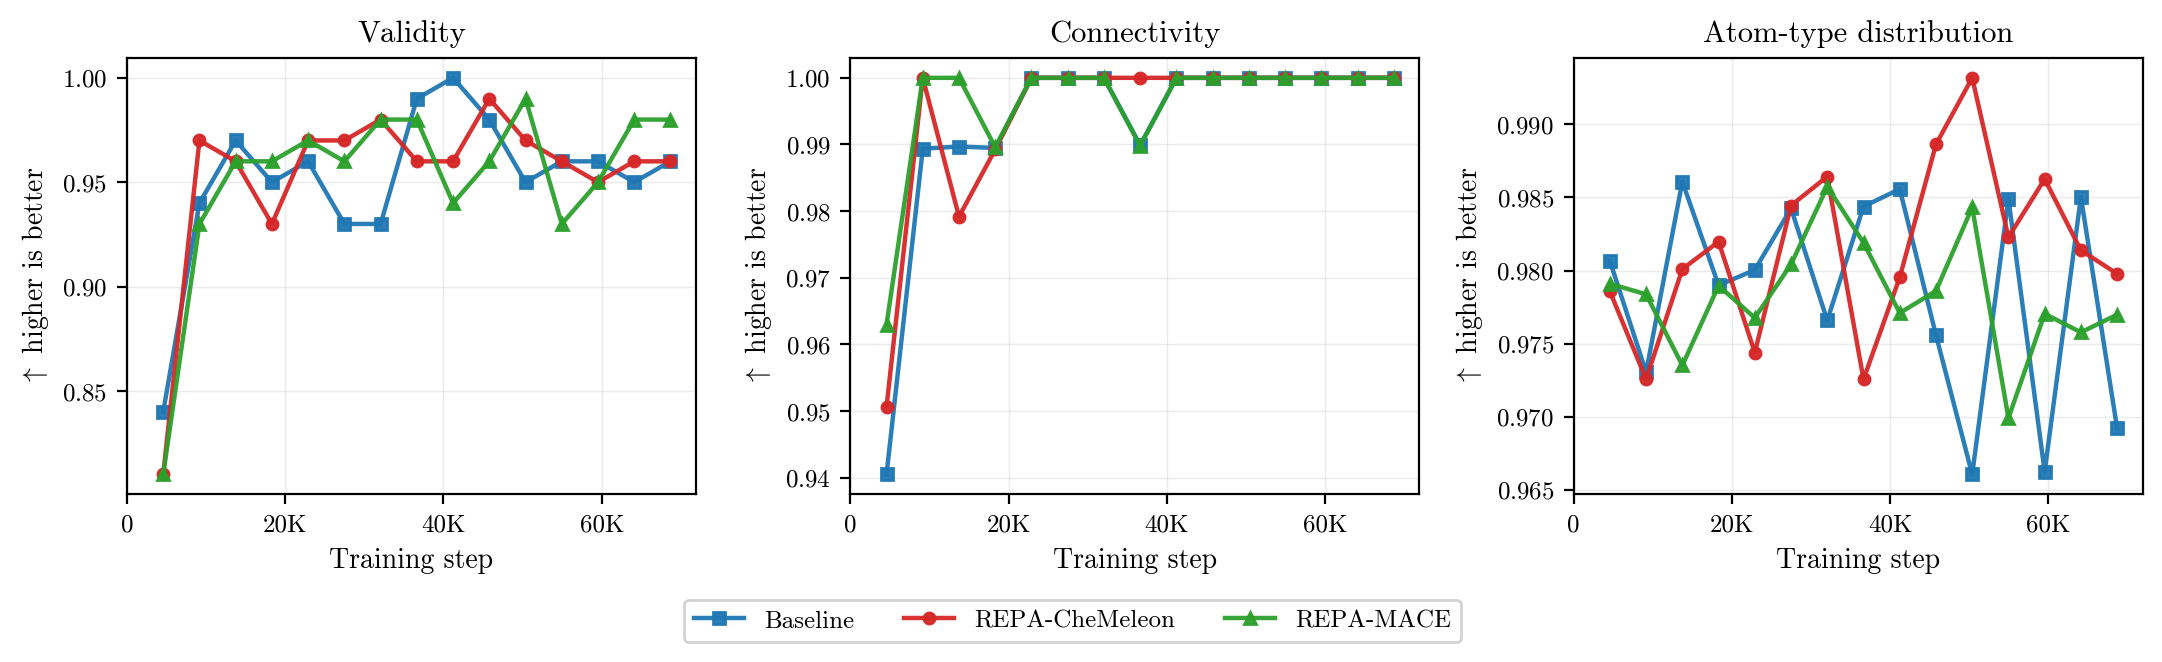
\includegraphics[width=\textwidth]{figures/fig5_1_tabasco_curves.png}
\caption{\textbf{REPA does not accelerate generation quality over the baseline.} Generation quality on GEOM-drugs (100 molecules sampled per epoch during training), plotted over training step across the range all three runs reach. The baseline and both REPA variants track together and reach near-ceiling on every axis within the first few thousand steps, leaving no headroom for alignment to fill. The metric is the in-training estimate, so values differ slightly from the final-checkpoint evaluation of Table~\ref{tab:tabasco-gen}.}
\label{fig:tabasco-curves}
\end{figure}


% Tabasco generation metrics -- \input{} from report-draft.tex Ch5.
\begin{table}[tbp]
\centering
\small
\begin{tabular}{l c c c c c c c}
\toprule
\textbf{Model} & \textbf{Steps} & \textbf{Valid.} & \textbf{Conn.} & \textbf{Uniq.} & \textbf{Div.} & \textbf{Nov.} & \textbf{FCD}~$\downarrow$ \\
\midrule
Baseline                     & 151k & 0.980 & 0.998 & 1.000 & 0.886 & 0.966 & \textbf{5.61} \\
\midrule
REPA-CheMeleon               & 73k  & 0.972 & 0.999 & 1.000 & 0.882 & 0.961 & 7.43 \\
REPA-MACE                    & 69k  & 1.000 & 0.995 & 0.996 & 0.884 & 0.977 & 6.81 \\
\bottomrule
\end{tabular}
\caption{\textbf{REPA brings no measurable gain over the baseline.} The quality metrics are saturated, sitting at or near their ceiling for baseline and variants alike. On FCD, the only metric with headroom, both variants are worse. (1{,}000 sampled molecules; higher-is-better except FCD ($\downarrow$). \emph{Steps} is the training step at evaluation; the baseline trained ${\sim}2{\times}$ longer, but the quality metrics plateau early, so the unequal steps do not make the comparison unfair (\S\ref{sec:tabasco-results}). One run per variant.)}
\label{tab:tabasco-gen}
\end{table}


\section{Discussion}
\label{sec:tabasco-diagnosis}

\textbf{The null result suggests this regime offers neither headroom nor usable teachers.} Under the original hypothesis, REPA~\cite{REPA} alleviates a representation bottleneck and therefore accelerates improvements on generation quality. However, this needs two conditions. First, there must be \emph{headroom}: a gap in what the generator represents or produces, for the alignment to fill. Second, there must be a \emph{usable teacher}: an encoder that encodes representational information that differs from what the trunk already has and transfers to the generative task. In this regime, neither condition holds.

\textbf{The first condition fails on the metric surface.} The generation quality axes are saturated, as \S\ref{sec:tabasco-results} showed. The representation side is saturated too --- the trunk already encodes what our descriptors capture --- so this regime happens to be closed on both.

\textbf{The second condition fails on both encoders, for opposite reasons (Table~\ref{tab:tabasco-probe}).} From our linear probes, we learn that CheMeleon decodes the descriptors almost perfectly in isolation ($R^2$ up to $0.99$). But the baseline trunk \emph{already decodes them well} ($0.64$--$0.92$), because they are 2D-graph quantities and the trunk sees the graph. CheMeleon's signal therefore overlaps with what the model already has. Moreover, FCD ultimately scores the inferred 2D graph --- the very information the trunk already holds --- so even on the one metric with headroom, CheMeleon adds nothing new.

MACE presents the contrary problem. It is genuinely 3D, but it encodes only a narrow, energy-tuned slice of \emph{local} atomic chemistry. The global descriptors we probe sit outside that slice, so they are largely undecodable from its mean-pooled embedding ($R^2$ near zero, save a weak $0.31$ on LogP). Its signal differs from the trunk's, but does not transfer. To calibrate the scale, note that an untrained random-weight encoder (Dummy) already decodes molecular weight at $R^2 = 0.82$, simply because weight tracks atom count. MACE falls below even this floor on three of the four descriptors.

% Tabasco descriptor-regression probe (R^2) -- \input{} from report-draft.tex Ch5.
\begin{table}[tbp]
\centering
\small
\begin{tabular}{l c c c c}
\toprule
\textbf{Source} & \textbf{MolWt} & \textbf{LogP} & \textbf{\#Rings} & \textbf{\#RotBonds} \\
\midrule
\multicolumn{5}{l}{\textit{Frozen encoders (the REPA targets in isolation)}} \\
CheMeleon (2D) & 0.993 & 0.988 & 0.995 & 0.989 \\
MACE (3D)      & 0.022 & 0.307 & 0.081 & $-0.014$ \\
Dummy          & 0.822 & 0.160 & 0.432 & 0.345 \\
\midrule
\multicolumn{5}{l}{\textit{Generator trunk (the model's internal representation)}} \\
Baseline             & 0.920 & 0.713 & 0.742 & 0.636 \\
REPA-CheMeleon       & 0.943 & 0.669 & 0.736 & 0.606 \\
REPA-MACE            & 0.935 & 0.703 & 0.704 & 0.582 \\
REPA-MACE (tradeoff) & 0.955 & 0.730 & 0.732 & 0.666 \\
\bottomrule
\end{tabular}
\caption{\textbf{Linear-probe $R^2$ reveals little representational difference between REPA and the baseline.} The baseline trunk already captures what CheMeleon learns, while MACE's embedding is too narrow to decode these descriptors. Hence, neither makes for a usable REPA target. ($R^2$ for four RDKit descriptors, on held-out molecules; \S\ref{sec:tabasco-metrics}; $n{=}1$ seed.)}
\label{tab:tabasco-probe}
\end{table}


\textbf{Forcing the signal in does not rescue it either.} As a final test, we replaced the additive regulariser with a convex \emph{tradeoff} loss, $(1-\lambda)\cdot\mathcal{L}_{\text{gen}} + \lambda\cdot\mathcal{L}_{\text{REPA}}$. This deliberately down-weights the flow-matching loss to force the model to adopt the encoder's representation. Even so, the effect on generation is negligible. MACE under the tradeoff loss still trails the baseline on FCD ($6.32$ versus $5.61$; Table~\ref{tab:tabasco-gen}). Its only mark is on the representation, where it is the only variant to beat the baseline on a majority of the descriptor probes (Table~\ref{tab:tabasco-probe}), but only by a small margin. Even when forced into the architecture, MACE leaves only a tiny trace in representation, and nothing in generation.

\textbf{When is REPA actually useful?} Our results sharpen the question on REPA's effectiveness rather than settling it. Under our setup, REPA does not help because the regime offers neither headroom nor a usable teacher. This is not evidence that REPA cannot help with molecular generation in principle. Indeed, we do not claim to have exhausted the REPA design space, and there may be other configurations that work well. But it does suggest the question has no single answer. Molecular generation is a broad domain of distinct regimes, and whether REPA helps may be decided within each, not across the whole. Read that way, REPA is not a single intervention, but a family of them.

Practically, we must look for a regime within the domain that satisfies these two conditions. Protein backbone generation presents an intriguing possibility on both fronts, and that is where we turn next.

\chapter{REPA on protein backbones}
\label{ch:proteina-study}


In this chapter, we expand the scope of our study on representation alignment from small molecules to much larger ones: proteins. In Chapter~\ref{ch:tabasco-study}, our efforts using REPA to generate small molecules yielded little demonstrable improvement, because the Tabasco~\cite{Tabasco} baseline already saturated most measures of generation quality, and because the encoders used were likely unhelpful. However, de-novo backbone design represents a more challenging task, as the data distribution of proteins is significantly larger, and the geometry of these structures is correspondingly more complex. In this context, we ask: \emph{can REPA accelerate or improve the training of Proteina~\cite{Proteina}, a flow-matching transformer-based protein backbone generator?}

\textbf{Our headline finding is that REPA accelerates convergence on the two key measures of protein generation quality.} This holds across both experimental and synthetic training-data regimes (Figure~\ref{fig:proteina-fid}). The one exception is designability on synthetic data, which the baseline already saturates under standard sampling (\S\ref{sec:proteina-datasets}). This chapter characterises \emph{what} happens and attempts to understand \emph{why}. We note that our objective here is to test whether the mechanism transfers at all, not to search for the optimal REPA configuration.

\emph{A caveat on unequal training and evaluation.} Given resource constraints, not every variant was trained for the same number of steps, or evaluated with the same number of seeds. We prioritised training and evaluating promising candidates. We flag where this shapes a comparison and read trends rather than single points.

\emph{Reading figures and tables in this chapter.} Unless otherwise specified, figures plot data from the PDB-trained $n\le 256$ data-regime (\S\ref{sec:proteina-datasets}) using 3 seeds; trajectories show the cross-seed mean, with shaded bands giving the min/max range. Every artefact notes its seed count in a trailing parenthetical. In tables, the baseline is usually an absolute value and each REPA row a $\Delta$ from it; \colorbox{green!20}{green} marks a change in the metric's good direction and \colorbox{red!15}{red} a change against it; \colorbox{green!42}{darker green} signals the best entry in a column; small $|\Delta|$ are left uncoloured.

% Figure -- headline FID + designability convergence. \input{} from Ch6.
\begin{figure}[tbp]
\centering
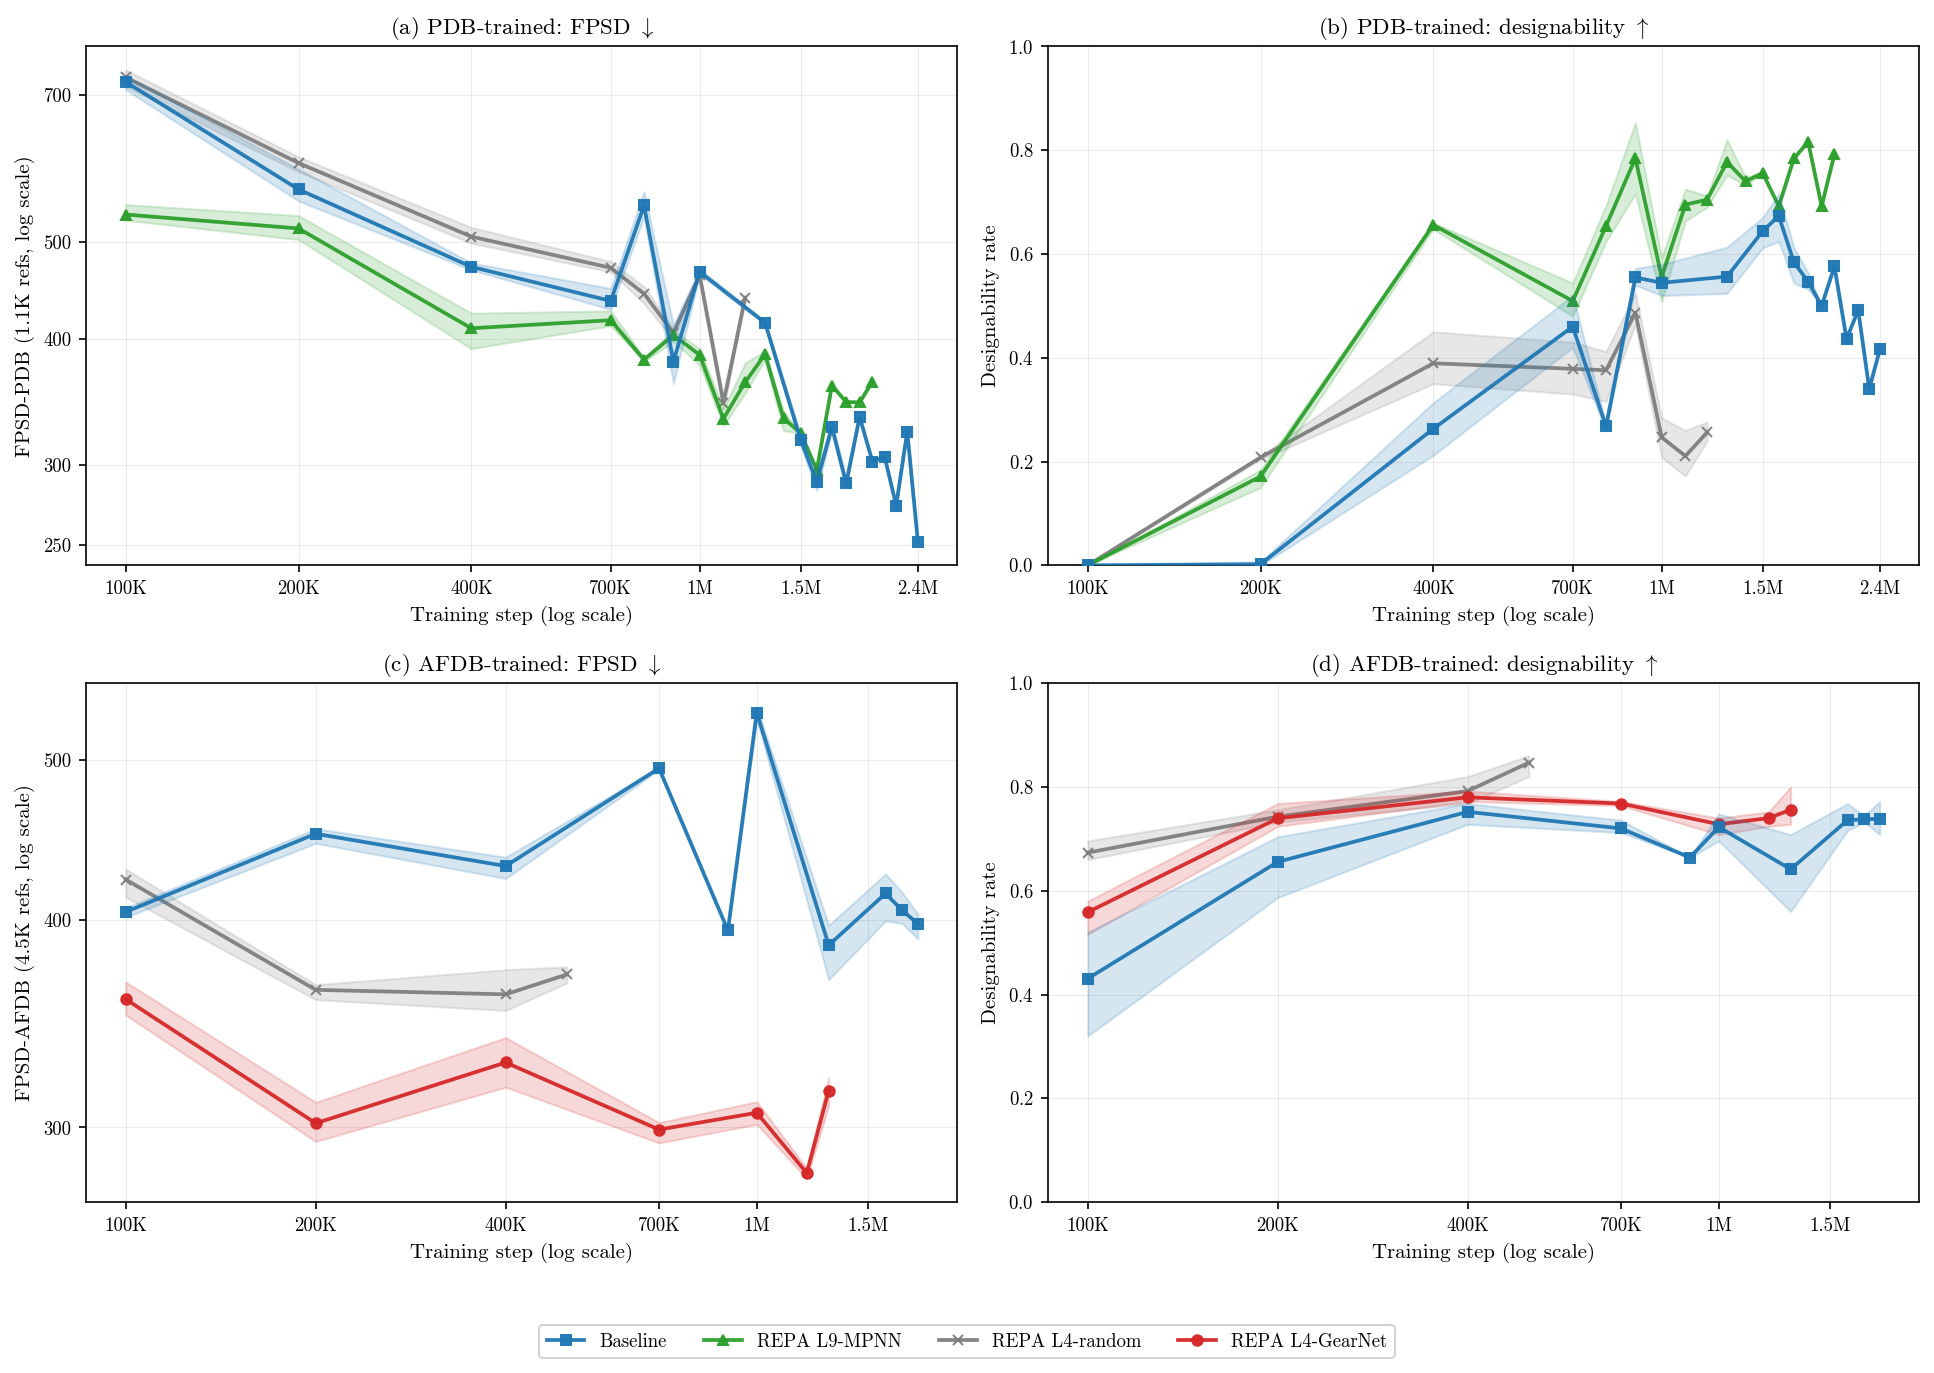
\includegraphics[width=\textwidth]{figures/fig01_fid_des_convergence.png}
\caption{\textbf{REPA accelerates both FID and designability, in both PDB (experimental) and AFDB (synthetic) data regimes.} The random-encoder control (grey) helps distinguish gains induced by regularisation alone from those induced mechanistically by an encoder's learned structure. While PDB retains a persistent designability gap, its baseline appears to catch up on FID after $\approx$1M steps; we examine this in \S\ref{sec:proteina-convergence}. ($n{\le}256$ models, 3 seeds; shaded bands show min/max.)}
\label{fig:proteina-fid}
\end{figure}


\section{Experimental setup}
\label{sec:proteina-setup}

We integrate REPA into Proteina~\cite{Proteina}, a 60M-parameter non-equivariant flow-matching generator of C$\alpha$ protein backbones (\S\ref{sec:protein}). Following \S\ref{sec:repa}, we attach a trainable projector at a chosen layer of the generator trunk (the transformer stack) that aligns the model's hidden states to a frozen external encoder.

\subsection{Datasets}
\label{sec:proteina-datasets}

We train in two data regimes that mirror the data-scarcity context motivating this report (Chapter~\ref{ch:intro}). The Protein Data Bank (PDB)~\cite{PDB} is the high-quality experimental source, but it is relatively scarce, containing on the order of hundreds of thousands of structures. The AlphaFold Database (AFDB)~\cite{AFDB} is the synthetic alternative containing hundreds of millions of AF2-predicted structures, but it is almost entirely unverified. We treat the datasets as two ends of a quality--scale axis. (We use the manually-curated Swiss-Prot subset of AFDB as a reproducible stand-in for the Foldseek-clustered TrEMBL subset on which Proteina was trained in the original presentation~\cite{Proteina}. This corpus contained data that has since been pruned from AFDB, and is hence inaccessible.)

Following Proteina~\cite{Proteina}, we train on the subset of chains with at most 256 residues; we represent this length-regime by $n{\le}256$. (We note that this represents only a property of the training datasets, not a bound on the length of the proteins that models trained on these datasets can generate.) Following this filter, the two training sets are comparable in size (PDB: 273{,}771 / 3{,}190 / 323 train/val/test chains; AFDB: 229{,}670 / 4{,}521 / 235). Appendix~\ref{ch:appendix} (Table~\ref{tab:setup-datasets}) contains further details on dataset composition. During training, we augment each backbone with a single random global rotation per sample.

\textbf{Different datasets in this domain carry different biases.} Trends in designability offer a clear example, as training on AFDB raises the in-silico-designability floor well above PDB at every setting we tested (\S\ref{sec:proteina-convergence}). This is the designability-proxy lineage effect of Chapter~\ref{ch:evaluation}: the test re-folds with models sharing AlphaFold2's lineage, so AlphaFold-like backbones are plausibly re-folded most confidently. We also note that both datasets feature some amount of structural similarity across training and evaluation subsets. We attempt to control for this in our evaluation protocol, as noted in \S\ref{sec:eval-protocol}.
\subsection{Models}

The base Proteina model comprises a stack of ten transformer layers (zero-indexed) that feeds a flow matching objective. Our experiments add a REPA loss to this design, as outlined in Table~\ref{tab:setup-model}.

\textbf{Encoder and injection-depth ablations.} Our narrative concentrates on the two encoders identified as most viable in Chapter~\ref{ch:profiling}: \emph{GearNet}~\cite{GearNet}, a structure encoder pretrained for CATH fold classification (checkpoint released with Proteina~\cite{Proteina}); and \emph{ProteinMPNN}~\cite{ProteinMPNN}, which encodes each residue's local inverse-folding environment. Each encoder is attached to the trunk in two layer-depth configurations: layer~4 (middle layer) and layer~9 (last layer). The remaining encoder and depth combinations are collected in Appendix~\ref{app:rep-full} (Table~\ref{tab:proteina-rep-full}). Figures presented in this chapter will typically feature the best performing model to serve as an illustrative example.

\textbf{Separating regularisation from mechanism.} A random-weights GearNet attached at layer 4, identical in architecture but never trained, serves as a control architecture in this chapter. We use this model to separate whatever REPA achieves merely due to the regularisation effect of adding an auxiliary loss from what it achieves through the encoder's \emph{learned} structural knowledge. Crucially, a trained encoder at the same layer~4 still outperforms the random one, so the learned-versus-random gap is not an artefact of injection depth (Appendix~\ref{app:rep-full}).

\textbf{Hyperparameters.} Our defaults largely follow the original image-domain REPA recipe~\cite{REPA}.

% Setup Table S2 -- model & REPA configuration. \input{} from report-draft.tex Ch6.
\begin{table}[tbp]
\centering
\small
\begin{tabular}{l l}
\toprule
\textbf{Property} & \textbf{Value} \\
\midrule
Generator        & Proteina (CAFlow), 60M parameters \\
Trunk            & 10-layer non-equivariant transformer; token dim 512, 8 heads \\
Parameterisation & raw C$\alpha$ coordinates (no architectural symmetry priors) \\
\midrule
Alignment loss   & cosine similarity, averaged per residue (Table~\ref{tab:setup-hparams}) \\
Projector        & 3-layer MLP, hidden dim 512 \\
Injection depth $\ell$ & layer 4 (middle) and layer 9 (last) of 10, zero-indexed \\
Encoder targets  & CA-GearNet (512-d, frozen) $\cdot$ ProteinMPNN $\cdot$ random-GearNet (control) \\
\bottomrule
\end{tabular}
\caption{Model configurations presented in this chapter. The
broader layer/encoder sweep is in Appendix~\ref{ch:appendix}.}
\label{tab:setup-model}
\end{table}
`'


\subsection{Metrics}
\label{sec:proteina-metrics}

The original hypothesis that motivated REPA for imaging~\cite{REPA} was that alleviating a \emph{representation} bottleneck would improve \emph{generation} quality. We seek to understand if the same mechanism applies in the molecular domain as well. Hence, along with estimating the quality of a model's generated samples, we are also interested in what the model comes to represent internally. To this end, we measure three families of metrics, as outlined below: representation quality, representation alignment, and generation quality (Table~\ref{tab:eval-protein}).

\textbf{Representation quality.} We use the three-task protein battery of Chapter~\ref{ch:evaluation} (inverse folding, dihedral error, CATH fold classification; Table~\ref{tab:eval-protein}). Because the three probes target largely orthogonal capabilities --- local chemical environment, local geometry, and global fold --- improving all of them at once is strong evidence of holistic representation quality. Among the CATH levels we headline on architecture (CATH-A): Class is too easy (top-1 saturates) and Topology too sparse (too many buckets, too few chains). We report all three for completeness, the patterns holding across them, and motivate the choice in Appendix~\ref{ch:appendix} (Table~\ref{tab:setup-cath}).

\textbf{Representation alignment.} This measures how close the trunk sits to a structural encoder, via CKNNA (\S\ref{sec:eval-probe}). As in the original REPA analysis~\cite{REPA} and a recent molecular extension~\cite{BoltzREPA}, we use it as a diagnostic --- a mechanistic lens on how REPA might produce its representation gains --- rather than a quantity we optimise or build claims on.

\textbf{Generation quality.} This is what ultimately matters, and we report it through the two-axis taxonomy of Chapter~\ref{ch:evaluation} --- tertiary/secondary structure crossed with whole set/designable subset --- laid out as supercolumns in our result tables: Quality, T-W, T-D, S-W, and S-D (Table~\ref{tab:eval-protein}). We report two headline metrics: designability and FPSD. We use this taxonomy to analyse REPA's effect on both the whole generated distribution and the designable subset.

Most of these metrics follow Proteina~\cite{Proteina}; the one we add, ssJSD-2D, is defined in Chapter~\ref{ch:evaluation}. As we explore in \S\ref{sec:proteina-anatomy}, REPA improves distribution match and whole-set diversity together, but may trade off tertiary-structure diversity within the designable subset.

\subsection{Evaluation protocol}
\label{sec:eval-protocol}

\textbf{Representation probing.} Following the probe principle of \S\ref{sec:eval-probe}, we fit probes to a frozen checkpoint's hidden states on clean inputs ($t{=}1$): the inverse-folding (IF) and dihedral probes per residue, the CATH probe per chain on mean-pooled representations. IF is a 20-way classification, while CATH-A is a $\sim$40-way one.

Each probe is fit on $1{,}000$ training chains. We evaluate the per-residue probes (inverse folding and dihedral) on a \emph{blinded} set of $\sim$325 proteins ($\sim$43k residues) held to under 30\% sequence identity to all training data, which removes both model- and probe-side leakage. The per-chain CATH probe needs many distinct chains spread across fold classes, which that small slice cannot supply, so we relax it to a \emph{probe-clean} evaluation on a larger validation set of $\sim$3{,}190 chains. We detail this scheme, and the model/probe leakage distinction it controls for, in Appendix~\ref{app:leakage}, and read rank-order and $\Delta$-from-baseline throughout this chapter.

\textbf{Representation alignment.} In \S\ref{sec:eval-probe}, we outlined how CKNNA scores how closely two representations share their nearest-neighbour structure. We compute it on clean ($t$=1) data from a fixed held-out batch, between the hidden states at every trunk layer and three domain-relevant encoders: GearNet, ProteinMPNN, and ESM2~\cite{ESM2}. We use $k{=}10$ neighbours over $10{,}000$ residues, and bracket each value with a subsample-without-replacement bootstrap (50 draws at 80\%; sampling with replacement would inflate the score through duplicate neighbour pairs). The absolute CKNNA values we record are small, an order of magnitude below image-domain REPA~\cite{REPA}, so we read the direction and layer structure of the effect, and its separation from the baseline, not its raw magnitude.

\textbf{Generation sampling.} Our generation evaluation follows the Proteina protocol~\cite{Proteina}, at a reduced sample budget. We record further details on the protocol in \S\ref{sec:eval-protein}.

For whole-set evaluations, we sample $1{,}125$ backbones per checkpoint --- 125 at each length in $\{50, 75, \dots, 250\}$ --- and compute metrics over all of them. Depending on the training regime, we use matching PDB or AFDB reference statistics.

For designability evaluations, 50 backbones at each length $\{50, 100, 150, 200, 250\}$ are inverse-folded with ProteinMPNN (8 sequences each), re-folded with ESMFold, and called designable when the self-consistency RMSD is below 2\,\AA{}. The designable-subset metrics (T-D, S-D) are then computed on the backbones that pass.

With this experimental testbed in place, the rest of the chapter investigates what the REPA construction changes with respect to baseline, and how that helps improve generation quality. We now turn to the results.

\section{Results}

\subsection{REPA improves representation quality asymptotically}
\label{sec:proteina-rep}

\textbf{At baseline, the flow-matching objective helps the model encode some useful representational information.} Figure~\ref{fig:proteina-rep} shows the results of probing our models along the three orthogonal axes of \S\ref{sec:proteina-metrics}: local chemical environment (inverse folding), local geometry (backbone dihedrals), and global fold (CATH classification, with CATH-A as our headline metric). The trained baseline consistently does better than both random features and an untrained Proteina trunk. This suggests that the flow-matching objective does indeed learn to \emph{represent} protein backbones as it learns to \emph{generate} them.

% Figure -- student representation quality vs training step. \input{} from Ch6.
\begin{figure}[tbp]
\centering
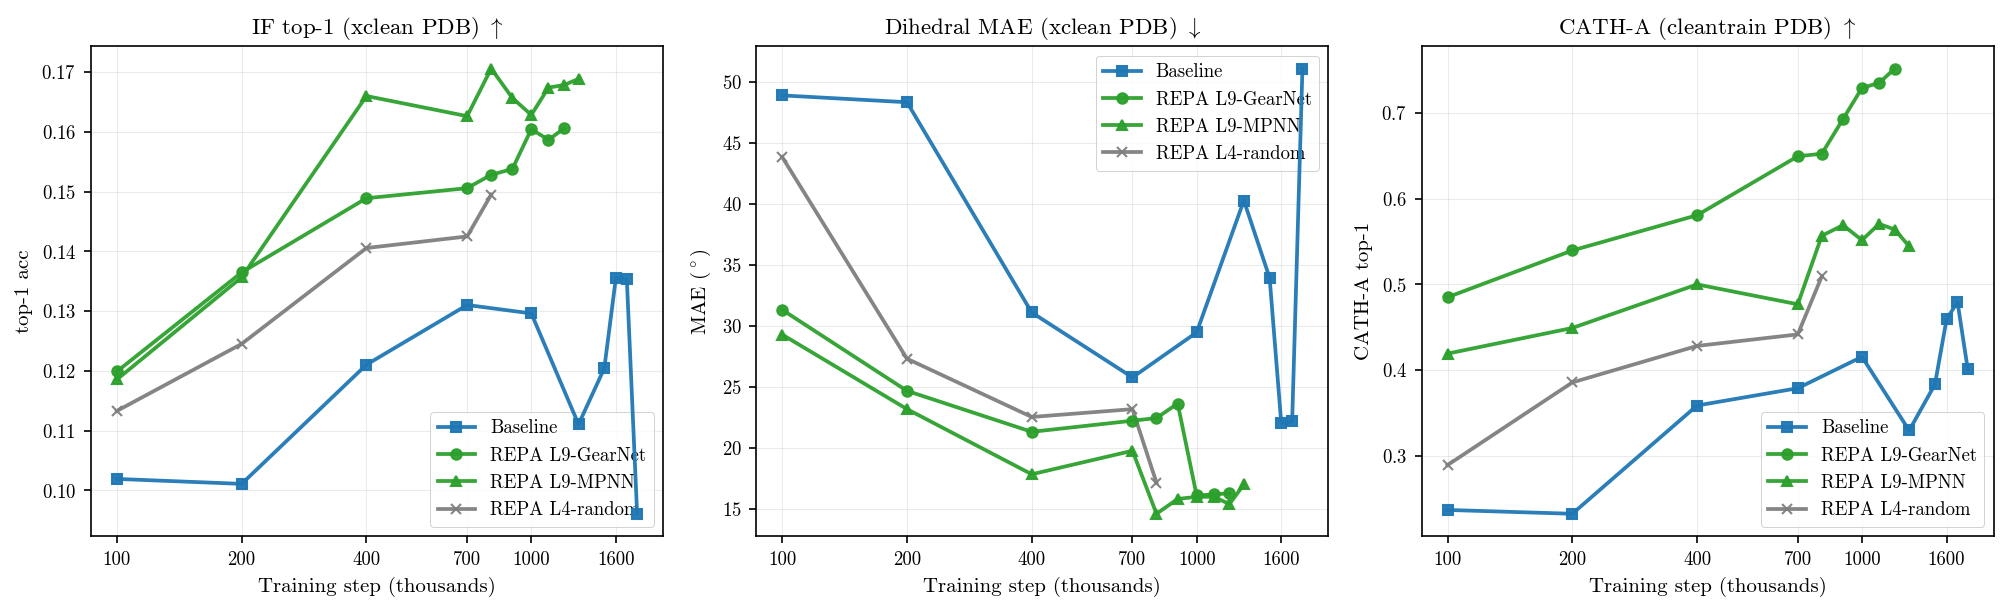
\includegraphics[width=\textwidth]{figures/fig02_representation.png}
\caption{\textbf{REPA lifts the trunk's representation quality asymptotically.} REPA variants open a quality gap over baseline that never closes; the random control gains least, evidence of genuine transfer rather than regularisation. (L9-GearNet and L9-MPNN shown; $3$ probe seeds; protocol in Appendix~\ref{app:leakage}.)}
\label{fig:proteina-rep}
\end{figure}


\textbf{Every trained-encoder REPA variant improves representational capacity, consistently and durably.} Each lifts all three probes substantially above the baseline, from the very beginning of training, and the difference persists. This is an asymptotic gap that the baseline never closes across 1.8M steps, not just a head start or an accelerated convergence pattern. This gap confirms one of the hypotheses posited in the original REPA presentation~\cite{REPA}: an alignment target during training can fill the representational headroom left by the flow-matching objective.

\textbf{Every encoder routes representation gain differently.} REPA-GearNet consistently wins the fold probes, while REPA-MPNN edges the per-residue inverse-folding probe (Table~\ref{tab:proteina-rep}). This pattern follows what we would expect a-priori, given the tasks that each encoder has been specifically trained for. This ties into our emerging theme on the multi-factorial nature of representation learning in the molecular domain~(Chapter~\ref{ch:evaluation}). No single encoder captures every factor, so the choice of alignment target is also a choice over the representational factor a model designer wishes to emphasise. We establish this routing on PDB-trained models and report the AFDB results in Appendix~\ref{app:rep-afdb}.

% Auto-generated by tables/scripts/make_rep_quality.py --- do not hand-edit.
% Single late checkpoint at 1000k (latest step all four share at 3 seeds).
\begin{table}[tbp]
\centering
\small
\setlength{\tabcolsep}{5pt}
\begin{tabular}{lccccc}
\toprule
 & & & \multicolumn{3}{c}{\textbf{CATH top-1 acc.\,$\uparrow$}} \\
\cmidrule(lr){4-6}
\textbf{Variant} & \textbf{IF top-1\,$\uparrow$} & \textbf{dihedral MAE\,(\,$^\circ$\,)\,$\downarrow$} & C & A & T \\
\midrule
Baseline & $0.129_{\pm0.004}$ & $31.5_{\pm1.7}$ & $0.724_{\pm0.013}$ & $0.408_{\pm0.007}$ & $0.332_{\pm0.009}$ \\
REPA L4-random & \rd{$-0.010_{\pm0.002}$} & $+3.9_{\pm3.1}$ & \gd{$+0.049_{\pm0.005}$} & $+0.011_{\pm0.008}$ & $-0.005_{\pm0.013}$ \\
REPA L9-GearNet & \gd{$+0.023_{\pm0.002}$} & \gb{$-6.4_{\pm0.3}$} & \gb{$+0.153_{\pm0.009}$} & \gb{$+0.267_{\pm0.006}$} & \gb{$+0.415_{\pm0.017}$} \\
REPA L9-MPNN & \gb{$+0.026_{\pm0.002}$} & $-5.6_{\pm4.0}$ & \gd{$+0.081_{\pm0.006}$} & \gd{$+0.063_{\pm0.003}$} & \gd{$+0.106_{\pm0.026}$} \\
\bottomrule
\end{tabular}
\caption{\textbf{REPA offers persistent and encoder-routed representation advantages.} At a representative late checkpoint, REPA-GearNet wins the fold probes (CATH C/A/T) decisively, while REPA-MPNN edges the per-residue probe (IF). The random control gains least and does not help the per-residue probes, evidence the effect is genuine structural transfer rather than regularisation. We headline on CATH-A and report C and T for completeness. (Single checkpoint at 1.0M --- the latest training step all four variants share at three seeds, and a representative point on the baseline trajectory rather than a transient swing; $n{=}3$ seeds, with $\pm$ half the seed range. Best-layer linear probe at $n_\text{train}{=}1000$ (cross-database set for IF/dihedral, cleantrain for CATH); dihedral carries the widest seed spread, so the per-residue read rests on IF. Colour marks significance against the combined seed spread: green better (darker $=$ column-best), red worse, uncoloured within seed noise. Persistence across training is shown in Figure~\ref{fig:proteina-rep}.)}
\label{tab:proteina-rep}
\end{table}


\textbf{REPA offers a mechanistic effect beyond just regularisation.} Our random-weights control improves on the baseline for the fold probes (CATH), but not for the per-residue ones. Where it helps, this may be because \emph{any} regularisation generically improves representation capacity, or because even an untrained message-passing network imposes some geometric priors that aid the trunk. However, the trained encoders consistently perform far better. This sharpens the case for a genuine mechanistic effect, as regularisation alone is not the whole story.

\textbf{The random control behaves as we expected a saturated target would.} In \S\ref{sec:profiling-protein} we characterised the random-init encoder as saturated, based on its high-floor signature. This makes the alignment loss cheatable, in that the trunk can optimise the loss without learning anything useful (\S\ref{sec:profiling-framework}). Our results bear this out. The random encoder's cosine similarity saturates higher than every trained model's --- ${\approx}0.89$ against ${\approx}0.80$ for a trained GearNet at the same layer~4 on PDB. Yet this near-perfect alignment buys the least representation quality of any variant, and no FPSD or designability gain (\S\ref{sec:proteina-convergence}).

\subsection{A diagnostic check on alignment}
\label{sec:proteina-alignment}

Following Yu et al.~\cite{REPA} and recent in-domain work~\cite{BoltzREPA}, we investigate the mechanism that may be driving REPA's representation quality gains by quantifying the representation alignment it induces. Using CKNNA~\cite{PlatonicRep}, we score how closely our models' per-residue geometry matches that of three domain-specific encoders: GearNet and ProteinMPNN, our two alignment targets in this chapter; and ESM2~\cite{ESM2}, which we align to only in our ablations, not in the models presented here. We note that we study alignment only as a diagnostic, and not to make claims about REPA's utility.

\textbf{REPA lifts alignment above the random floor, albeit at low magnitude.} The baseline sits at the random floor at every layer (CKNNA $\approx 0$), while REPA separates from it cleanly, suggesting that its hidden states do move towards the encoder's (Figure~\ref{fig:proteina-cknna}a). This serves as a minimal check that the construction changes model behaviour. However, the magnitude of this signal is small. Peak per-residue CKNNA (bootstrap median) is $\approx 0.02$--$0.05$, on a scale where self-alignment is $1$. We therefore read the pattern, not its size, and stake no strong claim on these numbers.

% Figure -- per-layer CKNNA alignment + Platonic off-diagonal. \input{} from Ch6.
\begin{figure}[tbp]
\centering
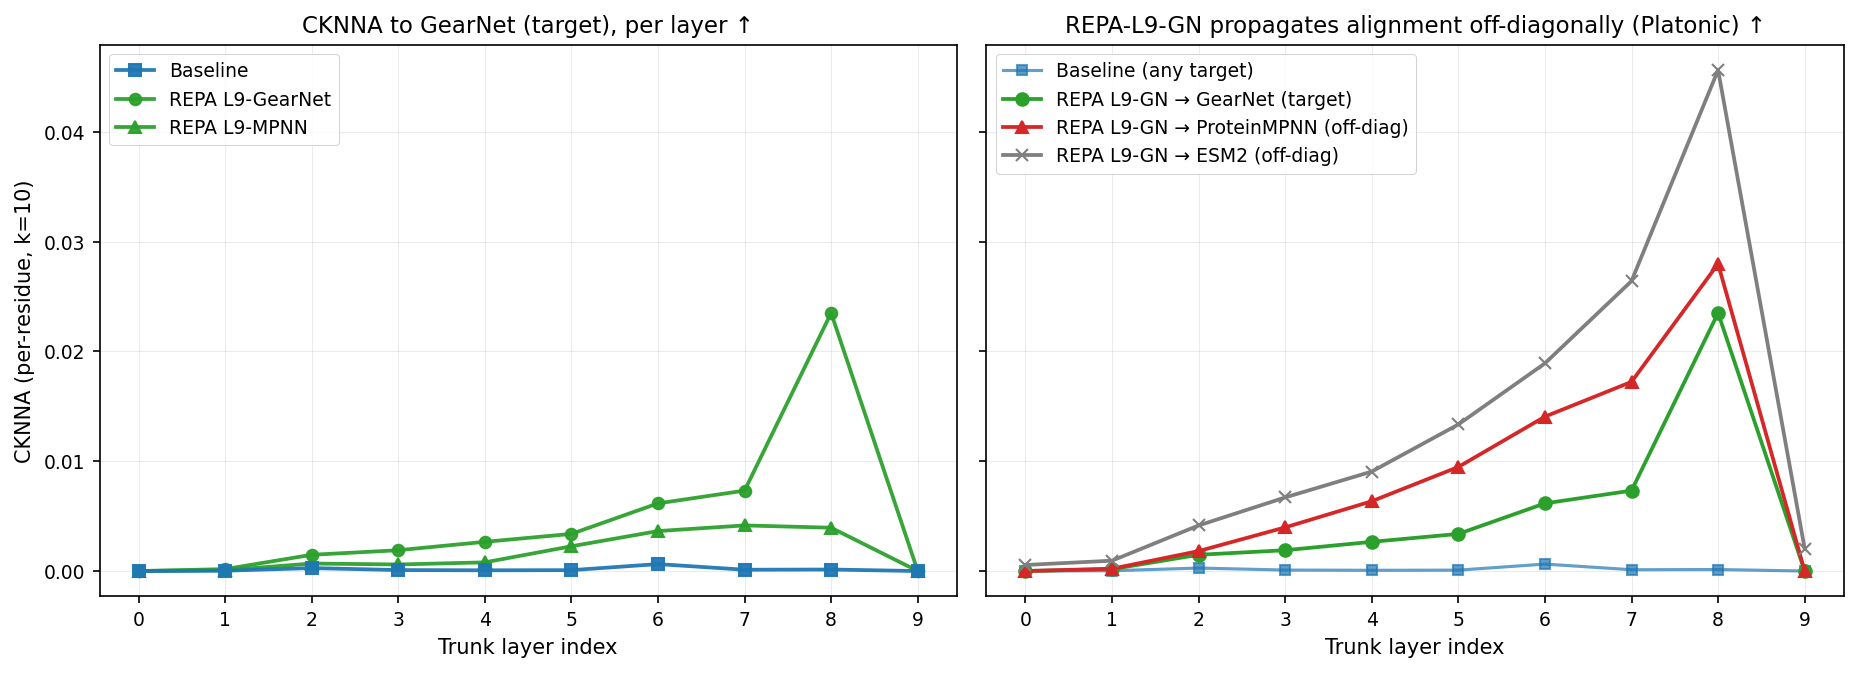
\includegraphics[width=\textwidth]{figures/fig03_alignment.png}
\caption{\textbf{REPA pulls the trunk's geometry toward the encoder's --- and toward encoders it was never trained on (Platonic convergence).} The baseline sits at the random floor at every layer (CKNNA $\approx 0$); REPA lifts per-residue alignment into a smooth profile that peaks one layer below the injection point and collapses at the velocity-output layer, cleanly separated from the baseline by the subsample bootstrap. Aligning to GearNet alone also pulls the trunk toward ProteinMPNN and ESM2 --- the off-diagonal Platonic signature, with ESM2 the strongest attractor. Absolute alignment is small (peak $\approx 0.02$--$0.05$ against $1$ for self-alignment), so we read direction and layer structure, not magnitude; the per-protein signal is far weaker and we do not claim a fold-level benefit. ($n{\le}256$ PDB, step 1M, $t{=}1.0$; per-residue CKNNA, $k{=}10$.)}
\label{fig:proteina-cknna}
\end{figure}


\textbf{Aligning to one encoder nudges the trunk towards others as well.} Every REPA variant we tested raises alignment to all three encoders, including those it was not aligned to (full model$\times$encoder matrix in Appendix~\ref{app:cknna}). A GearNet-aligned trunk, for example, also moves closer to ProteinMPNN and ESM2~\cite{ESM2} (Figure~\ref{fig:proteina-cknna}b), suggesting that REPA-induced alignment is not merely circular self-alignment. One possible explanation for this phenomenon is the \emph{Platonic representation hypothesis}~\cite{PlatonicRep}. This idea suggests that models trained on related data converge toward a shared representation. In this framework, REPA may be nudging the trunk toward a common structural representation that several encoders approximate, rather than toward any single encoder.

\subsection{In the short run, REPA accelerates generation quality in both experimental and synthetic data regimes}
\label{sec:proteina-convergence}
\label{sec:proteina-genrep}

Here, we outline our headline results using the \emph{Quality} metrics of our suite, FPSD and designability (as in Table~\ref{tab:eval-protein}). A deeper analysis of generation quality along tertiary- and secondary-structure decomposition follows in \S\ref{sec:proteina-anatomy}.

\textbf{Every REPA variant gives generation quality an early head start.} Table~\ref{tab:proteina-speedup} shows how at 400K steps, every variant already leads the baseline on PDB designability, by $+48\%$ to $+149\%$. Most variants also lead on FPSD in both regimes, with the best at $+28\%$. AFDB designability is the lone exception, for the proxy reason given in \S\ref{sec:proteina-datasets}.

% Auto-generated by tables/scripts/make_speedup_table.py --- do not hand-edit.
\begin{table}[tbp]
\centering
\small
\begin{tabular}{l c c}
\toprule
\textbf{Variant} (last ckpt) & \textbf{Acceleration} (@400K) & \textbf{Long run} (best) \\
\midrule
\multicolumn{3}{l}{\textit{AFDB FID $\downarrow$} --- baseline (to 1.7M) @400K 431, best 386 within 2.0M} \\
GearNet-L4 (1.2M) & \gd{$+24\%$ (328)} & \gd{$+27\%$ (282 @1.2M)} \\
GearNet-L9 (900K) & \gd{$+28\%$ (313)} & \gd{$+19\%$ (313 @400K)} \\
MPNN-L4 (1.1M) & \rd{$-10\%$ (477)} & \rd{$-8\%$ (416 @1.0M)} \\
MPNN-L9 (1.5M) & \gd{$+18\%$ (352)} & \gd{$+9\%$ (352 @400K)} \\
Random control (500K) & \gd{$+18\%$ (353)} & \gd{$+9\%$ (353 @400K)} \\
\midrule
\multicolumn{3}{l}{\textit{AFDB designability $\uparrow$} --- baseline (to 1.7M) @400K 0.75, best 0.75 within 2.0M} \\
GearNet-L4 (1.2M) & \gd{$+4\%$ (0.78)} & \gd{$+4\%$ (0.78 @400K)} \\
GearNet-L9 (900K) & \rd{$-4\%$ (0.72)} & \gd{$+3\%$ (0.77 @800K)} \\
MPNN-L4 (1.1M) & \rd{$-9\%$ (0.68)} & \rd{$-8\%$ (0.69 @700K)} \\
MPNN-L9 (1.5M) & \rd{$-6\%$ (0.71)} & \gd{$+2\%$ (0.77 @700K)} \\
Random control (500K) & \gd{$+9\%$ (0.82)} & \gd{$+9\%$ (0.82 @400K)} \\
\midrule
\multicolumn{3}{l}{\textit{PDB FID $\downarrow$} --- baseline (to 2.4M) @400K 472, best 288 within 2.0M} \\
GearNet-L4 (1.0M) & \gd{$+7\%$ (440)} & \rd{$-50\%$ (432 @1.0M)} \\
GearNet-L9 (1.6M) & \gd{$+28\%$ (341)} & \rd{$-11\%$ (319 @700K)} \\
MPNN-L4 (1.6M) & \rd{$-8\%$ (512)} & \rd{$-14\%$ (329 @1.6M)} \\
MPNN-L9 (2.0M) & \gd{$+13\%$ (410)} & \rd{$-3\%$ (297 @1.6M)} \\
Random control (1.2M) & \rd{$-7\%$ (506)} & \rd{$-22\%$ (351 @1.1M)} \\
\midrule
\multicolumn{3}{l}{\textit{PDB designability $\uparrow$} --- baseline (to 2.4M) @400K 0.26, best 0.67 within 2.0M} \\
GearNet-L4 (1.0M) & \gd{$+98\%$ (0.52)} & \gd{$+4\%$ (0.70 @700K)} \\
GearNet-L9 (1.6M) & \gd{$+97\%$ (0.52)} & \rd{$-7\%$ (0.63 @800K)} \\
MPNN-L4 (1.6M) & \gd{$+124\%$ (0.59)} & \gd{$+5\%$ (0.71 @1.6M)} \\
MPNN-L9 (2.0M) & \gd{$+149\%$ (0.66)} & \gd{$+21\%$ (0.82 @1.8M)} \\
Random control (1.2M) & \gd{$+48\%$ (0.39)} & \rd{$-31\%$ (0.46 @900K)} \\
\bottomrule
\end{tabular}
\caption{\textbf{REPA accelerates generation quality over the baseline.} In some regimes it also wins the long run. (Values are percentage deltas from the baseline, with the absolute score in parentheses; acceleration is measured at 400K, the anchor of Figure~\ref{fig:proteina-genrep}, and the long run as each variant's best within a common 2.0M-step window; generation scores are means over up to three sampling seeds; $n{\le}256$; \colorbox{green!20}{green}/\colorbox{red!15}{red} = improvement/regression.)}
\label{tab:proteina-speedup}
\end{table}


\textbf{For the strongest variant per dataset, this early acceleration holds across the whole sampler-noise axis.} The lead is not an artefact of one inference recipe. Taking the strongest variant per dataset (Table~\ref{tab:proteina-speedup}), it reaches a higher level of \emph{both} FPSD and designability than the baseline at almost every sampler setting (Table~\ref{tab:proteina-sampler}). The lone exception is the degenerate $\gamma{=}0$ regime, where heavy noise correction inflates both models' divergence. This shows the acceleration is built into the learned model, not merely recovered at inference.

% Table -- sampler-noise robustness, per-gamma Delta. \input{} from Ch6.
\begin{table}[tbp]
\centering
\small
\setlength{\tabcolsep}{6pt}
\begin{tabular}{l|cccccc}
\toprule
$\Delta$ (REPA $-$ baseline) & ODE & $\gamma=0$ & $\gamma=0.35$ & $\gamma=0.45$ & $\gamma=0.5$ & $\gamma=1.0$ \\
\midrule
\multicolumn{7}{l}{\textit{PDB --- REPA L9-MPNN vs Baseline (step-matched cells).}}\\
Des $\uparrow$         & \gd{+0.06} & \gd{+0.07} & \gd{+0.16} & \gd{+0.18} & \gd{+0.15} & \gd{+0.04} \\
FID $\downarrow$        & \gd{$-$22}   & \gd{$-$1225} & \gd{$-$78}   & \gd{$-$77}   & \gd{$-$89}   & \gd{$-$131} \\
fJSD-A $\downarrow$     & \gd{$-$0.13} & \rd{+0.18} & \rd{+0.21} & \gd{$-$0.06} & \rd{+0.07} & \gd{$-$0.30} \\
ssJSD2D $\downarrow$    & \gd{$-$0.11} & \rd{+0.08} & \gd{$-$0.01} & \gd{$-$0.03} & \gd{$-$0.00} & \gd{$-$0.10} \\
\#Clust $\uparrow$      & \gd{+9}    & \gd{+8}    & \rd{$-$7}    & \gd{+4}    & \gd{+12}   & \gd{+2}  \\
\midrule
\multicolumn{7}{l}{\textit{AFDB --- REPA L4-GearNet vs Baseline (step-matched cells).}}\\
Des $\uparrow$          & \gd{+0.16} & \gd{+0.08} & \gd{+0.07} & \gd{+0.06} & \gd{+0.06} & \gd{+0.08} \\
FID $\downarrow$         & \gd{$-$102}  & \gd{$-$45}   & \gd{$-$133}  & \gd{$-$144}  & \gd{$-$132}  & \gd{$-$97} \\
fJSD-A $\downarrow$      & \gd{$-$0.31} & \rd{+0.28} & \gd{$-$0.94} & \gd{$-$1.06} & \gd{$-$0.92} & \gd{$-$0.24} \\
ssJSD2D $\downarrow$     & \gd{$-$0.04} & \gd{$-$0.19} & \gd{$-$0.13} & \gd{$-$0.13} & \gd{$-$0.10} & \gd{$-$0.03} \\
\#Clust $\uparrow$       & \gd{+32}   & \rd{$-$15}   & \rd{$-$27}   & \rd{$-$23}   & \rd{$-$21}   & \gd{+10} \\
\bottomrule
\end{tabular}
\caption{\textbf{REPA's gains are sampler-invariant in the middle band ($\gamma\in[0.35,0.5]$) and largely survive at the extremes --- a training-time effect that composes with the inference-time noise dial.} The large $-1225$ FID gain at $\gamma{=}0$ reflects the PDB baseline mode-collapsing at deterministic sampling. (Mean $\Delta$ = REPA $-$ baseline across step-matched cells per noise level, for the best PDB and AFDB variants; \colorbox{green!20}{green}/\colorbox{red!15}{red} = improvement/regression; negative is a win on lower-is-better metrics.)}
\label{tab:proteina-sampler}
\end{table}


\textbf{FPSD does not merely reward alignment to its own encoder.} FPSD reads generated sets through a GearNet fold classifier (\S\ref{sec:eval-protein}), which is one of the encoders we align to. A GearNet-aligned trunk might then gain on FPSD for free, pulled toward the metric's feature space. This does not bear out. On PDB, the best FPSD belongs to an MPNN-aligned model, not a GearNet-aligned one (Table~\ref{tab:proteina-13m}). The metric is rewarding a real distributional improvement, not self-alignment, which also lends credence to the GearNet-led FPSD wins we report on AFDB.

\textbf{This acceleration is consistent with the representation-bottleneck hypothesis.} Yu et al.~\cite{REPA} hypothesise that a model's representation quality and its generation quality are coupled, because it is learning both at once. In our PDB-trained models, this coupling is clear. Across checkpoints, representation and generation quality are positively correlated, and the strongest of these correlations survive controlling for training step (Table~\ref{tab:proteina-genrep-corr}). The same coupling holds on AFDB-trained models, and in the same encoder-matched form (Appendix~\ref{app:genrep-afdb}). If the two move together, then securing good representations early should secure good generation early as well. REPA reaches an asymptotically higher representation quality almost as soon as training begins (\S\ref{sec:proteina-rep}, Figure~\ref{fig:proteina-rep}), so this pattern is expected.

% Auto-generated by tables/scripts/make_genrep_corr.py --- do not hand-edit.
\begin{table}[tbp]
\centering
\small
\begin{tabular}{l cc cc}
\toprule
\textbf{Representation quality} & \multicolumn{2}{c}{\textbf{FPSD}} & \multicolumn{2}{c}{\textbf{Designability}} \\
\cmidrule(lr){2-3} \cmidrule(lr){4-5}
 & partial & raw & partial & raw \\
\midrule
Inverse folding (top-1) & +0.35 & +0.13 & +0.79 & +0.58 \\
Dihedral MAE & +0.42 & -0.07 & +0.76 & +0.32 \\
CATH-A & +0.20 & +0.07 & +0.48 & +0.35 \\
\bottomrule
\end{tabular}
\caption{\textbf{Better trunk representations track better generation --- strongly for designability, moderately for FPSD.} Partial Pearson correlation controlling for training step, with the raw value alongside; oriented so a positive value means better representation accompanies better generation. ($n{=}63$ checkpoints pooled over the baseline, the REPA variants, and the random control; generation is a $3$-seed mean, with only the single-seed late-tail checkpoints at $n{=}1$; probe single-seed; $1{,}125$ backbones/seed, $250$ for designability.)}
\label{tab:proteina-genrep-corr}
\end{table}


\textbf{REPA climbs the representation--
generation envelope faster than the baseline.} On the representation--generation curve posited by the bottleneck hypothesis, the early representation gains place REPA variants further along than the baseline at matched compute (Figure~\ref{fig:proteina-genrep}, shown for the strongest PDB variant). Hence, it reaches a given level of generation quality at less training. We interpret REPA as simply traversing this curve faster, rather than finding a new shortcut.

% Figure -- generation-vs-representation envelope (FID + designability). \input{} from Ch6.
\begin{figure}[tbp]
\centering
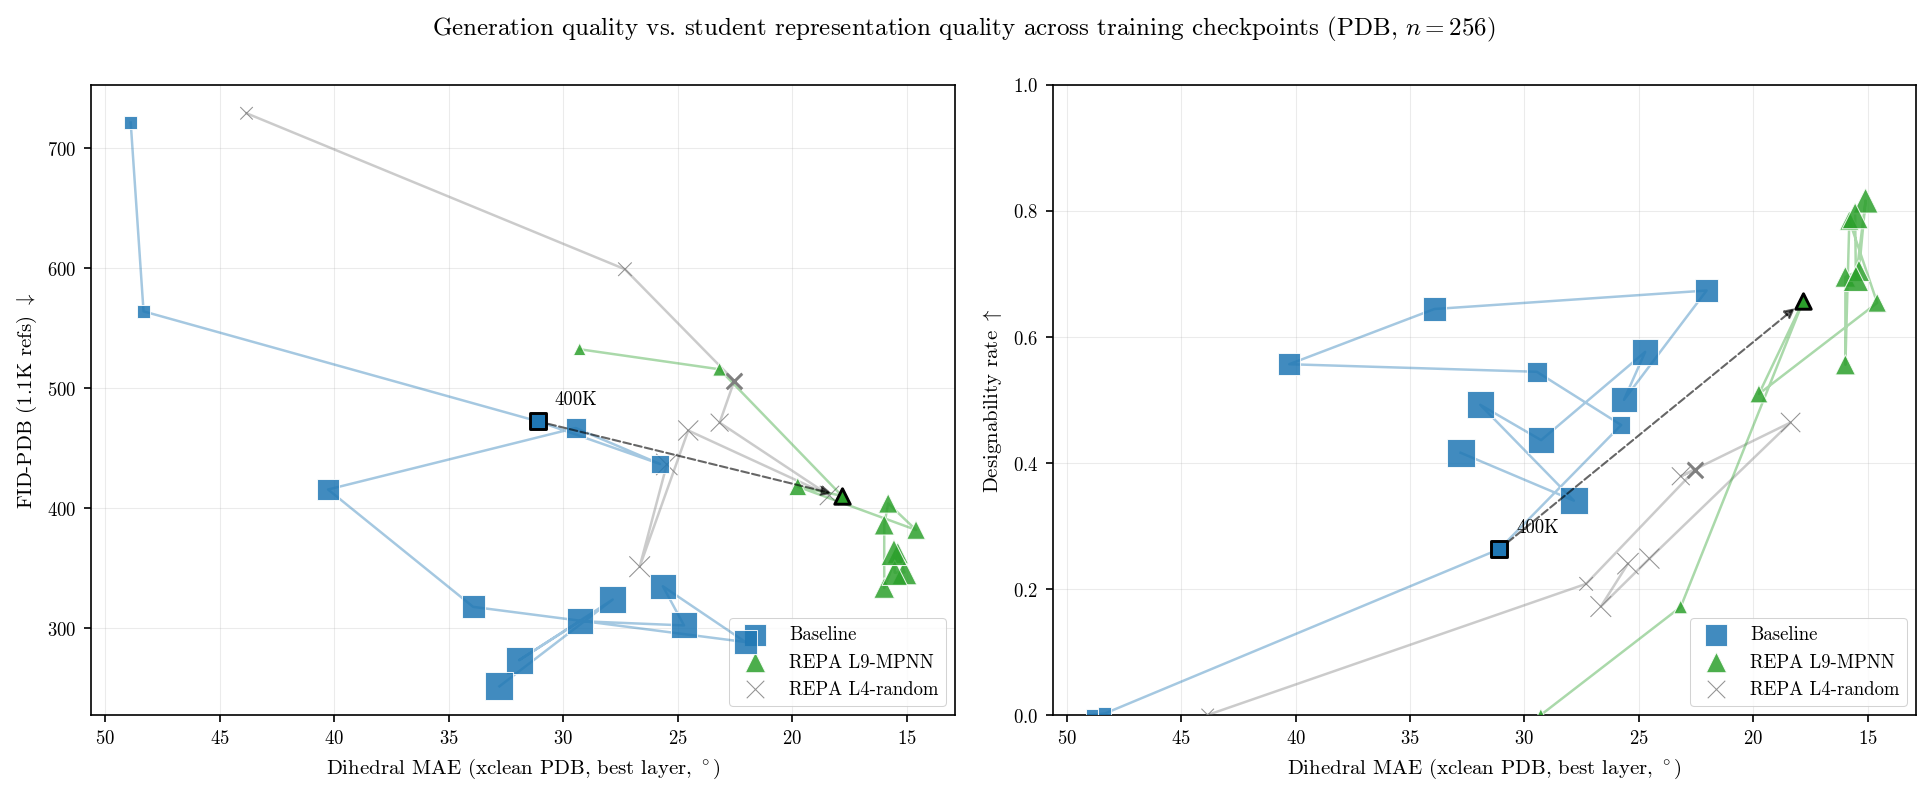
\includegraphics[width=\textwidth]{figures/fig04_fid_des_gen_vs_rep.png}
\caption{\textbf{Better student geometry buys better generation at equal compute --- direct evidence REPA relieves the representation bottleneck.} Generation quality against representation quality, $n=256$ PDB, one marker per checkpoint. The $x$-axis is student dihedral MAE (better to the right). \emph{Left:} FID-PDB (lower is better); \emph{right:} designability (higher is better). Baseline (blue squares), REPA L9-MPNN (green triangles), and the random control (grey $\times$) lie on a common band where better dihedral geometry accompanies better generation on both metrics. The dashed arrow connects baseline and L9-MPNN at matched training compute ($\approx 400$K steps), showing REPA delivering better generation quality for the same budget.}
\label{fig:proteina-genrep}
\end{figure}


\textbf{This representation--generation link is encoder-matched, suggesting the effect is encoder-specific, not generic regularisation.} Each encoder's generation gain lands on the axis where its representations are strongest. GearNet, the better fold encoder (\S\ref{sec:proteina-rep}), gives the larger acceleration on distribution match; MPNN, the better local encoder, gives the larger acceleration in designability (Table~\ref{tab:proteina-speedup}). Such axis-matching would be unlikely under a generic auxiliary loss, but we do not claim proof of causality.


\subsection{In the long run, REPA gains are data-regime dependent}
\label{sec:proteina-distribution}
\label{sec:proteina-anatomy}
\label{sec:proteina-modulation}

The short-run REPA-induced acceleration we observe in our headline metrics, FPSD and designability, is universal. Nearly every variant across both data regimes displays the same pattern (\S\ref{sec:proteina-convergence}). The long run is more contingent. Deep into training, REPA's gain becomes \emph{data-regime dependent}, which highlights the experimental--synthetic distinction that motivates our report and our experimental design (Chapter~\ref{ch:intro}, \S\ref{sec:proteina-datasets}). The choice of alignment target matters too, but the encoder that helps is dictated by the regime rather than chosen independently of it.

\textbf{Each data regime leaves a different gap, and REPA fills the one it is given.} On synthetic (AFDB) data, designability comes readily, partly by construction (\S\ref{sec:proteina-datasets}), while matching the fold distribution is the harder problem. On experimental (PDB) data the reverse holds, as the baseline already matches the distribution well, but leaves room on designability. Figure~\ref{fig:proteina-fid} depicts how REPA's long-run advantage shows wherever the gap is: on distribution match for AFDB, on designability for PDB. We note that designability on AFDB gains as well, but the improvement is small relative to the FPSD gain.

% Centerpiece Table -- 1.3M snapshot (post-1M-dip). \input{} from Ch6.
% Requires \gd/\rd macros and \usepackage[table]{xcolor} from the preamble.
% Built 2026-06-10 from existing eval data; 4 cells pending fresh gen-eval on
% existing checkpoints (PDB L4-random, PDB L4-GearNet; AFDB L9-GearNet, AFDB
% L4-MPNN) -- SLURM job 30352629 (array 0-3), output ->
% results/variance/n256_13m_backfill/. 1 cell unfillable (AFDB L4-random: no
% checkpoint past 800K). Column set follows the 700K table (no whole-set pwTM
% column: not computed at 1.3M). When job lands: rerun jsonl_to_tsv / clean +
% the centerpiece builder at step 1300000, fill the 4 rows, then swap the
% report \input from table_proteina_1m -> table_proteina_13m.
\begin{table}[tbp]
\centering
\small
\setlength{\tabcolsep}{4pt}
\resizebox{\textwidth}{!}{%
\begin{tabular}{lccccccccc}
\toprule
& \multicolumn{2}{c}{\textbf{Quality}}
& \multicolumn{2}{c}{\textbf{T-W}}
& \multicolumn{2}{c}{\textbf{T-D}}
& \textbf{S-W}
& \multicolumn{2}{c}{\textbf{S-D}} \\
\cmidrule(lr){2-3}\cmidrule(lr){4-5}\cmidrule(lr){6-7}\cmidrule(lr){8-8}\cmidrule(lr){9-10}
\textbf{Variant (1.3M)}
& Des\,$\uparrow$ & FPSD\,$\downarrow$
& fJSD-A\,$\downarrow$ & fS-A\,$\uparrow$
& \#Clust\,$\uparrow$ & pwTM\,$\downarrow$
& ssJSD2D\,$\downarrow$
& ssJSD2D\,$\downarrow$ & $\beta$-strand\,\%\,$\uparrow$ \\
\midrule
\multicolumn{10}{l}{\textit{PDB-trained.}}\\
Baseline       & 0.56 & 416 & 0.95 & 6.06 & 107 & 0.16 & 0.31 & 0.43 & 0.09 \\
REPA L4-random \textit{\scriptsize(1.2M)} & \rd{$-$0.32} & \rd{+21} & \gd{$-$0.37} & \rd{$-$0.07} & \rd{$-$54} & \rd{+0.03} & \gd{$-$0.16} & \gd{$-$0.06} & \gd{+0.03} \\
REPA L4-GearNet \textit{\scriptsize(1.0M)} & \rd{$-$0.10} & \rd{+17} & \gd{$-$0.41} & \gd{+1.29} & \rd{$-$20} & +0.01 & \gd{$-$0.16} & \gd{$-$0.04} & $-$0.01 \\
REPA L9-GearNet & \rd{$-$0.07} & \gd{$-$22} & \gd{$-$0.26} & \gd{+1.44} & \rd{$-$49} & \rd{+0.12} & \gd{$-$0.22} & \gd{$-$0.22} & \gd{+0.17} \\
REPA L4-MPNN   & \gd{+0.06} & \rd{+73} & \gd{$-$0.13} & \gd{+0.44} & \rd{$-$15} & \rd{+0.08} & \gd{$-$0.14} & \gd{$-$0.13} & \gd{+0.10} \\
REPA L9-MPNN   & \gd{+0.22} & \gd{$-$29} & \gd{$-$0.10} & \gd{+0.84} & \gd{+9} & \rd{+0.12} & \gd{$-$0.18} & \gd{$-$0.21} & \gd{+0.13} \\
\midrule
\multicolumn{10}{l}{\textit{AFDB-trained.}}\\
Baseline       & 0.64 & 386 & 1.63 & 5.45 & 114 & 0.18 & 0.10 & 0.20 & 0.13 \\
REPA L4-random \textit{\scriptsize(0.5M)} & \gd{+0.21} & \gd{$-$15} & \gd{$-$0.07} & \rd{$-$0.35} & \gd{+39} & +0.01 & \rd{+0.06} & $-$0.01 & +0.01 \\
REPA L4-GearNet & \gd{+0.11} & \gd{$-$71} & \gd{$-$0.67} & \gd{+2.14} & +0.0 & +0.02 & \gd{$-$0.06} & \gd{$-$0.09} & +0.03 \\
REPA L9-GearNet \textit{\scriptsize(1.0M)} & \gd{+0.08} & \gd{$-$93} & \gd{$-$0.50} & \gd{+1.54} & \rd{$-$30} & \rd{+0.07} & \gd{$-$0.07} & \gd{$-$0.14} & \gd{+0.06} \\
REPA L4-MPNN \textit{\scriptsize(1.1M)} & \gd{+0.05} & \rd{+72} & \rd{+0.30} & \rd{$-$0.48} & \rd{$-$10} & \rd{+0.07} & +0.01 & \gd{$-$0.06} & +0.01 \\
REPA L9-MPNN   & \gd{+0.12} & +1 & \gd{$-$0.09} & \rd{$-$0.37} & \gd{+37} & $-$0.00 & \rd{+0.05} & \gd{$-$0.04} & $-$0.02 \\
\bottomrule
\end{tabular}}
\caption{\textbf{Read within each regime: on AFDB REPA lifts the whole-set distribution cleanly; on PDB the whole-set gains come with a more concentrated designable subset.} Whole-set distribution match (FPSD, fJSD-A) and diversity (fS-A) favour REPA in both regimes; within the designable subset, REPA's pwTM rises above the baseline across the PDB variants but not the AFDB ones. Compare rows within a regime block, not across them. FPSD uses the training dataset as its reference in each case. This is a fixed checkpoint across all variants; Figure~\ref{fig:proteina-diversity-trend} tracks the representative variant across training. (Rows tagged with a step, e.g.\ \textit{\scriptsize(1.0M)}, are placeholders from that variant's latest available checkpoint, pending the 1.3M eval; AFDB L4-random has no checkpoint past 800K.)}
\label{tab:proteina-13m}
\end{table}


\textbf{On synthetic data, REPA learns a genuinely better model.} Table~\ref{tab:proteina-13m} captures the state of our models after 1.3M training steps. At this snapshot, the strongest long-run AFDB variant (identified in Table~\ref{tab:proteina-speedup}, long-run column), REPA-L4-GearNet, beats the baseline on Quality and whole-set (T-W, S-W) metrics at once, \emph{at no meaningful cost to designable-subset metrics} (T-D and S-D). This represents a true pushing of the designability--diversity envelope (\S\ref{sec:protein-tradeoffs}). The $0.02$ rise in designable pwTM is within the baseline's own seed-to-seed scatter, while the designability quality gains clear it (Appendix~\ref{app:13m-ranges}). This makes REPA-L4-GearNet the canonically better model under that framework, not merely a different point on the same envelope. This is learned model behaviour, not a sampler artefact. The same pattern survives the deterministic ODE limit, which reads the velocity field with no injected noise (Appendix~\ref{app:ode}). The random-weights control marks the boundary of a genuine gain. At just $0.5$M steps, the least training of any variant, it posts the AFDB block's best designability ($+0.21$). Yet it improves FPSD only marginally and regresses on fold similarity (fS-A). That designability bump reflects the auxiliary loss, not structural transfer.

\textbf{On experimental data, REPA finds a different spot on the designability--diversity envelope.} At the 1.3M snapshot, across variants, REPA delivers whole-set gains (T-W, S-W) while pushing the designable subset toward $\beta$-strand content (S-D). However, designable diversity (T-D) drops, as the model appears to collapse onto fewer distinct $\beta$-rich folds (Table~\ref{tab:proteina-concentration}). This $\beta$-driven dynamic of secondary-structure enhancement and loss of tertiary-structure diversity is far stronger on PDB. The performance of the strongest long-run variant, REPA-L9-MPNN (identified in Table~\ref{tab:proteina-speedup}, long-run column), makes the resultant trade-off clear. While REPA increases designability on PDB, it does so by losing diversity, instead of pushing the frontier out as with AFDB.

% Table -- beta-stratified designable concentration (the T-D trade-off). \input{} from Ch6.
% Trimmed 2026-06-11 to baseline + strongest variant per regime (PDB L9-MPNN,
% AFDB L4-GearNet) to illustrate the regime difference cleanly; the all-variant
% "REPA-wide" breadth lives in Table 6.6's T-D column. Source:
% results/variance/beta_stratified_diversity.json (exp_beta_stratified_diversity.py).
% Absolute pwTM; colour marks REPA vs same-block/step/bin baseline: red=more
% concentrated, green=more diverse, |delta|<0.05 uncoloured. Single-seed.
\begin{table}[tbp]
\centering
\small
\setlength{\tabcolsep}{7pt}
\begin{tabular}{lcccccc}
\toprule
\textbf{Designable pwTM\,$\downarrow$} & \multicolumn{3}{c}{\textbf{400K steps}} & \multicolumn{3}{c}{\textbf{1.3M steps}} \\
\cmidrule(lr){2-4}\cmidrule(lr){5-7}
\textbf{Variant} & $\beta{<}10$ & $10$--$25$ & $\beta{\ge}25$ & $\beta{<}10$ & $10$--$25$ & $\beta{\ge}25$ \\
\midrule
\multicolumn{7}{l}{\textit{PDB-trained}}\\
Baseline        & 0.16 & 0.15 & 0.21 & 0.15 & 0.23 & 0.13 \\
REPA L9-MPNN    & 0.16 & \rd{0.21} & \rd{0.29} & 0.19 & 0.23 & \rd{0.69} \\
\midrule
\multicolumn{7}{l}{\textit{AFDB-trained}}\\
Baseline        & 0.19 & 0.22 & 0.16 & 0.13 & 0.26 & 0.14 \\
REPA L4-GearNet & 0.16 & 0.26 & 0.17 & \rd{0.22} & 0.26 & \rd{0.20} \\
\bottomrule
\end{tabular}
\caption{\textbf{On PDB, REPA concentrates the $\beta$-rich designable folds onto fewer modes; on AFDB it does not.} The effect is specific to the most $\beta$-rich bin ($\beta{\ge}25$): PDB-L9-MPNN climbs from $0.29$ (400K) to $0.69$ (1.3M) while its baseline diversifies to $0.13$. Lower-$\beta$ bins and AFDB-L4-GearNet barely move. Designable-subset pairwise TM, lower\,=\,more diverse; columns bin by $\beta$-strand fraction (\%). ($n{=}1$ seed; $250$ backbones/seed, designable subset.)}
\label{tab:proteina-concentration}
\end{table}


\textbf{The optimal alignment target follows from the data regime.} Alignment with ProteinMPNN lifts per-sample designability, while alignment with GearNet lifts the fold distribution (\S\ref{sec:proteina-convergence}). PDB's gap is in designability, so ProteinMPNN wins there, with REPA-L9-MPNN proving the best long-run PDB variant. AFDB's gap is in distribution match, so REPA-L4-GearNet proves stronger. For REPA in a multi-factorial and multi-scale domain like molecules, the data regime dictates which encoder pays off.

\subsection{What we do not claim}
\label{sec:proteina-scope}

Several tempting claims do not survive our data, and we flag them here.

\begin{itemize}
  \item \emph{No asymptotic generation quality win on experimental data.} REPA accelerates PDB convergence, but the lead is transient. The baseline matches REPA's FPSD plateau by ${\sim}1.4$M steps and edges below it by $1.6$M (\S\ref{sec:proteina-convergence}). The durable advantage on distribution match is on synthetic (AFDB) data, where the baseline plateaus poorly.
  \item \emph{Co-movement, not mediation.} Representation and generation quality move together. We do not claim one formally causes the other, but we note that the pattern is consistent with the representation bottleneck hypothesis (\S\ref{sec:proteina-genrep}).
  \item \emph{Unconditional generation only.} Every experiment here is unconditional: we specify a target length but never a fold class or other structural motif. We do not claim these dynamics carry over to the conditional setting (\S\ref{sec:flow-matching}).
  \item \emph{No claim of optimality.} We do not search the configuration space for the best setup of layer, weight, or encoder. With limited compute, variants were also trained to different horizons, so some late comparisons rest on fewer checkpoints than others; we flag these in the text. The question here is whether the mechanism works at all, not how to tune it for maximum gain (\S\ref{sec:proteina-setup}).
  \item \emph{Pre-convergence regime by design.} Our models are likely under-trained against a fully converged Proteina. We make no claim about behaviour at convergence. The claim is about acceleration. The early-training boost is real, and that early regime is the one we care about, even if the asymptotic picture differs after much longer training (\S\ref{sec:proteina-convergence}).
\end{itemize}

\section{Discussion}
\label{sec:proteina-discussion}

\textbf{We show that REPA accelerates Proteina's convergence on generation quality, and suggest that this works through representation.} Every trained encoder teaches the trunk to represent structural characteristics that the flow-matching loss never learns on its own. For each encoder, this representation gain is mirrored in the generation gain, on the axis where that encoder is strongest. A random-weights control suggests that the mechanism is indeed genuine structural transfer, not the side effect of an auxiliary loss. Its alignment loss drops more than any trained encoder, yet this buys the least representation quality, and no meaningful generation gain (\S\ref{sec:proteina-rep}).

\textbf{Unlike small molecules, protein backbone generation meets the conditions for REPA.} Our small-molecule study set out two conditions for REPA to help (\S\ref{sec:tabasco-diagnosis}). There must be headroom, a gap in what the generator represents or produces for the alignment to fill. And there must be a usable teacher, an encoder whose signal differs from what the trunk already learns and transfers to the generative task. Small molecules met neither, and we observed a null result (Chapter~\ref{ch:tabasco-study}). Proteins meet both. The null there and the success here are two sides of the same coin.

\textbf{In molecular generation, REPA is a family of encoder-mediated interventions, not a single mechanism.} There is no single best pre-trained encoder. Each buys a different representational factor, so the best choice is likely use-case specific --- or, as in our case, data-regime specific (\S\ref{sec:proteina-modulation}). The dataset establishes the bottleneck, and the encoder routed to that factor is the one that helps.

\textbf{Geometric convergence between encoders need not make them interchangeable.} The alignment signal we measure is small, so we raise this only as a talking point (\S\ref{sec:proteina-alignment}). Nevertheless, we observe that aligning to one encoder nudged the trunk toward the others too, which may read as a pull toward a shared structural representation, in the spirit of the Platonic representation hypothesis~\cite{PlatonicRep}. Yet the encoders are plainly not interchangeable. Each routes its gain to a different factor (\S\ref{sec:proteina-anatomy}). The two sit together if the encoders share a common core but differ in what they emphasise above it, and REPA transfers both.

\textbf{One thread we leave open is whether alignment outlives its early purpose.} REPA appears to help most early, and its benefit may fade later in training. On PDB, two observations point this way: the distribution-match lead is transient, and the designable subset concentrates mid-training (\S\ref{sec:proteina-anatomy}). One reading is that the encoder is a fixed target, so once the trunk has taken what it offers, continued alignment keeps pulling it toward the encoder's own, narrower distribution. A similar arc is reported in image diffusion, where one idea proposes to stop alignment early to preserve its early gains and mitigate its later downsides~\cite{HASTE}. We see a superficially similar pattern in molecules, but we need more evidence to know whether the resemblance is real, and if this solution would help.

We carry these results, and the contrast with the small-molecule study of Chapter~\ref{ch:tabasco-study}, into this report's conclusion in Chapter~\ref{ch:conclusions}.

\chapter{Conclusions}
\label{ch:conclusions}



Our work is motivated by a tension in the field of molecular generation, as outlined in Chapter~\ref{ch:intro}. Following a wider trend in machine learning, molecular generation has traded hard structural priors for architectural simplicity, and curated experimental data for synthetic scale. Both phenomena dilute the structural signal available to models during training, which exacerbates their representation bottleneck~\cite{REPA} and causes poor convergence behaviour. Representation alignment (REPA) is potentially one cheap way to provide models this signal and accelerate training. This report investigates two questions: does REPA work in the molecular domain, and when does it work at all?

In this concluding chapter, we collect threads from across our report to build answers. We also raise new questions and future work that follow from our report, and invite a larger discussion in this field.

\section{Does REPA work in the molecular domain?}
\label{sec:concl-domain}

Our report documents two regimes, small molecules and protein backbones, and presents a different answer for each. On small molecules, no REPA variant left
a measurable mark on Tabasco (Chapter~\ref{ch:tabasco-study}). On protein backbones, REPA accelerated Proteina's convergence on the two key measures of generation quality, likely by improving the representations learned by the model (Chapter~\ref{ch:proteina-study}).

What explains these divergent behaviours? At root, the two regimes represent completely different chemistry. A small drug-like molecule and a folded protein backbone are not the same kind of object, even if their in-silico parameterisations appear to squash these distinctions at first glance. That chemistry sets the combinatorial space a generator must cover: modest and topology-dominated for small molecules, vast and hierarchical for proteins. The former presents a more learnable target, so its generators mature sooner. Indeed, by the time we test REPA, the evaluation metrics for small-molecule generation sit at ceiling, and the baseline Tabasco model already learns the information contained in our external encoders. Protein generation, working in a far larger space, is far from this point, and therefore benefits from the intervention.

The protein-backbone result is ultimately a statement about training efficiency, and it pays off along two axes.

The first is \emph{acceleration}: for a fixed compute budget, REPA reaches better generation quality in both the experimental (PDB) and synthetic (AFDB) regimes. Early in training, every variant already leads the baseline on designability, and most lead on distribution match (FPSD) in both regimes (\S\ref{sec:proteina-convergence}). A cheap auxiliary signal buys faster convergence, which is highly valuable in a data-scarce, prior-light field.

The second axis is \emph{asymptotics}: whether that early lead survives to convergence. Here the answer is not uniform, and it follows the data regime. The two regimes leave their headroom in different places. Synthetic (AFDB) data yields designability cheaply, but leaves the fold distribution hard to match. Experimental (PDB) data is the reverse, with a baseline that already matches the distribution but leaves room on designability (\S\ref{sec:proteina-distribution}). REPA's lasting gain lands wherever that gap is. On AFDB the distribution-match lead is permanent, because the baseline plateaus there. On PDB that same lead eventually closes, as the baseline catches up (\S\ref{sec:proteina-convergence}).

Both axes point the same way as a data-efficiency story. REPA always buys a faster climb, and can offer a lasting advantage when the baseline struggles most. The field's frontier --- larger synthetic corpora, longer backbones, the all-atom setting --- is where the generation problem is hardest and an unaided baseline has ground to make up. This may also be where REPA's payoff is greatest, and where it should be tested next.

\section{When does REPA work?}
\label{sec:concl-when}

The discussion above already hints at our answer, which is that REPA works when two
conditions hold together. The evaluation surface must leave \emph{headroom} for
a gain to register, and the encoder must be a \emph{suitable teacher} --- it
must carry structural information the generator does not already learn cheaply.

In this framework, our small-molecules study showed little promise because generation and representation quality metrics were already saturated, and the trunk already learned everything our encoders carried. Indeed, the problem of generating structurally plausible small molecules in-silico appears largely solved. To set appropriate expectations about what this means, we note that structural plausibility is only one desideratum among the many a real design campaign cares about (\S\ref{sec:primer}), and it is arguably the most tractable of them. The properties that actually determine a molecule's utility --- how it binds a target, metabolises, or synthesises --- are downstream of plausibility and far less settled. Moreover, all of this is measured in an in-silico sandbox that is itself a coarse stand-in for real chemistry. The saturated metrics do not suggest that we have mastered small-molecule generation, but that one tractable sub-problem of it looks solved under proxies that are far removed from the wet lab. But this suffices to leave REPA nothing to add.

Protein backbone generation presents a more challenging task, where both representation and generation metrics are unsaturated, and determining teacher suitability remains difficult. In Chapter~\ref{ch:evaluation}, we propose a new framework in which to interpret the vast array of relevant metrics, which are complex both in isolation and in their relationships with each other. We also frame the central dynamic that characterises a generator's quality, the \emph{designability--diversity} trade-off, and the distinction between merely moving along such an envelope and pushing it outward. In Chapter~\ref{ch:profiling}, we then propose a set of heuristics to estimate the utility of an encoder as a REPA teacher. We investigate the \emph{information} content of a suite of pre-trained encoders, the \emph{relevance} of that content to the generative task, and the mathematical \emph{conditioning} of their embeddings, and use the most promising candidates in the studies that follow. We note that the approach we propose here is domain-agnostic. The questions we raise are purely statistical, and can be asked of any encoder in any domain with a few modifications.

However, the molecular domain presents unique challenges in how multi-factorial and multi-scale its representations are, especially in contrast to images (\S\ref{sec:eval-multifactorial}). In this light, our work also presents a new view on REPA: it is not a single mechanism, but rather a \emph{family of interventions}. Every pre-trained encoder emphasises a different factor, so the choice of alignment target is also a choice over the structural factor one seeks to enhance.

\section{Open questions}
\label{sec:conc-open-questions}

We close by looking ahead, and proposing new directions based on our work.

\textbf{Does REPA work in other scientific domains?} Our report opened by placing this work in the wider arc of generative machine learning for the sciences (Chapter~\ref{ch:intro}). The same paradigm of prior-light models, sparse data, and multi-scale representation recurs across many scientific fields. For example, in fluid mechanics, diffusion models are learning to generate turbulent flow fields~\cite{TurbulenceDiffusion}. Alleviating the representation bottleneck could open the door for more efficient and performant models here, following our work with proteins.

\textbf{Does our encoder profiling framework generalise?} Singh et al.~\cite{SpatialStructure} ask the which-encoder question for vision, and answer it with structural metrics tied to the image grid. We attempt to generalise this analysis into a set of domain-agnostic heuristics. An open question is whether these are two views of a single, canonical characterisation of what makes a good alignment target. We propose retrospectively analysing published REPA work across domains, to see if the framework offers useful guidance.

We read our contribution not as a verdict that REPA accelerates protein backbone generation, but as a principled framework for assessing how to improve generative models for science more broadly. With that aspiration, we hope to raise more interesting research questions than we answer, and to push the evolution of this exciting space.

\label{lastcontentpage}


\begin{thebibliography}{99}


\bibitem{DDPM}
Jonathan Ho, Ajay Jain, Pieter Abbeel.
\textit{Denoising Diffusion Probabilistic Models}. NeurIPS 2020.
\href{https://arxiv.org/abs/2006.11239}{arXiv:2006.11239}.

\bibitem{FlowMatching}
Yaron Lipman, Ricky T.~Q.~Chen, Heli Ben-Hamu, Maximilian Nickel, Matt Le.
\textit{Flow Matching for Generative Modeling}. ICLR 2023.
\href{https://arxiv.org/abs/2210.02747}{arXiv:2210.02747}.

\bibitem{FMIntroLectures}
Peter Holderrieth and Ezra Erives.
\textit{An Introduction to Flow Matching and Diffusion Models}.
MIT 6.S184 lecture notes, 2025.
\href{https://diffusion.csail.mit.edu/}{diffusion.csail.mit.edu}.

\bibitem{FMGuide}
Yaron Lipman, Marton Havasi, Peter Holderrieth, Neta Shaul, Matt Le, Brian Karrer, Ricky T.~Q.~Chen, David Lopez-Paz, Heli Ben-Hamu, Itai Gat.
\textit{Flow Matching Guide and Code}. 2024.
\href{https://arxiv.org/abs/2412.06264}{arXiv:2412.06264}.


\bibitem{REPA}
Sihyun Yu, Sangkyung Kwak, Huiwon Jang, Jongheon Jeong, Jonathan Huang, Jinwoo Shin, Saining Xie.
\textit{Representation Alignment for Generation: Training Diffusion Transformers Is Easier Than You Think}. ICLR 2025.
\href{https://arxiv.org/abs/2410.06940}{arXiv:2410.06940}.

\bibitem{SpatialStructure}
Jaskirat Singh, Xingjian Leng, Zongze Wu, Liang Zheng, Richard Zhang, Eli Shechtman, Saining Xie.
\textit{What matters for Representation Alignment: Global Information or Spatial Structure?} 2025.
\href{https://arxiv.org/abs/2512.10794}{arXiv:2512.10794}.

\bibitem{REED}
Chenyu Wang, Cai Zhou, Sharut Gupta, Zongyu Lin, Stefanie Jegelka, Stephen Bates, Tommi Jaakkola.
\textit{Learning Diffusion Models with Flexible Representation Guidance}. 2025.
\href{https://arxiv.org/abs/2507.08980}{arXiv:2507.08980}.

\bibitem{BoltzREPA}
Hyosoon Jang, Hyunjin Seo, Yunhui Jang, Seonghyun Park, Sungsoo Ahn.
\textit{Boltz is a Strong Baseline for Atom-level Representation Learning}. 2026.
\href{https://arxiv.org/abs/2602.13249}{arXiv:2602.13249}.

\bibitem{VideoREPA}
Xiangdong Zhang, Jiaqi Liao, Shaofeng Zhang, Fanqing Meng, Xiangpeng Wan, Junchi Yan, Yu Cheng.
\textit{VideoREPA: Learning Physics for Video Generation through Relational Alignment with Foundation Models}. 2025.
\href{https://arxiv.org/abs/2505.23656}{arXiv:2505.23656}.

\bibitem{TARO}
Tri Ton, Ji Woo Hong, Chang D.~Yoo.
\textit{TARO: Timestep-Adaptive Representation Alignment with Onset-Aware Conditioning for Synchronized Video-to-Audio Synthesis}. ICCV 2025.
\href{https://arxiv.org/abs/2504.05684}{arXiv:2504.05684}.

\bibitem{CrystalREPA}
Chengqian Zhang, Yucheng Jin, Duo Zhang, Tiejun Li, Han Wang.
\textit{CrystalREPA: Transferring Physical Priors from Universal MLIPs to Crystal Generative Models}. 2026.
\href{https://arxiv.org/abs/2605.08960}{arXiv:2605.08960}.

\bibitem{DiffuseDisperse}
Runqian Wang and Kaiming He.
\textit{Diffuse and Disperse: Image Generation with Representation Regularization}. 2025.
\href{https://arxiv.org/abs/2506.09027}{arXiv:2506.09027}.

\bibitem{HASTE}
Ziqiao Wang, Wangbo Zhao, Yuhao Zhou, Zekai Li, Zhiyuan Liang, Mingjia Shi, Xuanlei Zhao, Pengfei Zhou, Kaipeng Zhang, Zhangyang Wang, Kai Wang, Yang You.
\textit{REPA Works Until It Doesn't: Early-Stopped, Holistic Alignment Supercharges Diffusion Training}. 2025.
\href{https://arxiv.org/abs/2505.16792}{arXiv:2505.16792}.


\bibitem{Proteina}
Tomas Geffner et al.
\textit{Proteina: Scaling Flow-based Protein Structure Generative Models}. ICLR 2025.
\href{https://arxiv.org/abs/2503.00710}{arXiv:2503.00710}.

\bibitem{Tabasco}
C.~Vonessen et al.
\textit{TABASCO: A Fast, Simplified Model for Molecular Generation with Improved Physical Quality}. 2025.
\href{https://arxiv.org/abs/2507.00899}{arXiv:2507.00899}.


\bibitem{REINVENT}
Marcus Olivecrona, Thomas Blaschke, Ola Engkvist, Hongming Chen.
``Molecular de-novo design through deep reinforcement learning''.
\textit{Journal of Cheminformatics} 9:48 (2017).
\href{https://doi.org/10.1186/s13321-017-0235-x}{doi:10.1186/s13321-017-0235-x}.

\bibitem{GENTRL}
Alex Zhavoronkov et al.
``Deep learning enables rapid identification of potent DDR1 kinase inhibitors''.
\textit{Nature Biotechnology} 37 (2019), pp.~1038--1040.
\href{https://doi.org/10.1038/s41587-019-0224-x}{doi:10.1038/s41587-019-0224-x}.

\bibitem{RFdiffusion}
Joseph~L. Watson et al.
``de-novo design of protein structure and function with RFdiffusion''.
\textit{Nature} 620 (2023), pp.~1089--1100.
\href{https://doi.org/10.1038/s41586-023-06415-8}{doi:10.1038/s41586-023-06415-8}.

\bibitem{Chroma}
John~B. Ingraham et al.
``Illuminating protein space with a programmable generative model''.
\textit{Nature} 623 (2023), pp.~1070--1078.
\href{https://doi.org/10.1038/s41586-023-06728-8}{doi:10.1038/s41586-023-06728-8}.

\bibitem{GNoME}
Amil Merchant et al.
``Scaling deep learning for materials discovery''.
\textit{Nature} 624 (2023), pp.~80--85.
\href{https://doi.org/10.1038/s41586-023-06735-9}{doi:10.1038/s41586-023-06735-9}.

\bibitem{MatterGen}
Claudio Zeni et al.
``A generative model for inorganic materials design''.
\textit{Nature} 639 (2025), pp.~624--632.
\href{https://doi.org/10.1038/s41586-025-08628-5}{doi:10.1038/s41586-025-08628-5}.

\bibitem{TurbulenceDiffusion}
Tim Whittaker, Romuald~A. Janik, Yaron Oz.
``Turbulence scaling from deep learning diffusion generative models''.
\textit{Journal of Computational Physics} 514 (2024), 113239.
\href{https://doi.org/10.1016/j.jcp.2024.113239}{doi:10.1016/j.jcp.2024.113239}.


\bibitem{MoleculeDiffusionSurvey}
Liang Wang, Chao Song, Zhiyuan Liu, Yu Rong, Qiang Liu, Shu Wu, Liang Wang.
\textit{Diffusion Models for Molecules: A Survey of Methods and Tasks}. 2025.
\href{https://arxiv.org/abs/2502.09511}{arXiv:2502.09511}.


\bibitem{ESM2}
Zeming Lin et al.
``Evolutionary-scale prediction of atomic-level protein structure with a language model''.
\textit{Science} 379.6637 (2023), pp.~1123--1130.
\href{https://doi.org/10.1126/science.ade2574}{doi:10.1126/science.ade2574}.

\bibitem{ProteinMPNN}
J.~Dauparas et al.
``Robust deep learning--based protein sequence design using ProteinMPNN''.
\textit{Science} 378.6615 (2022), pp.~49--56.
\href{https://doi.org/10.1126/science.add2187}{doi:10.1126/science.add2187}.

\bibitem{GearNet}
Zuobai Zhang, Minghao Xu, Arian Jamasb, Vijil Chenthamarakshan, Aurelie Lozano, Payel Das, Jian Tang.
\textit{Protein Representation Learning by Geometric Structure Pretraining}. ICLR 2023.
\href{https://arxiv.org/abs/2203.06125}{arXiv:2203.06125}.

\bibitem{ProteinWorkshop}
Arian R. Jamasb, Alex Morehead, Chaitanya K. Joshi, et al.
\textit{Evaluating Representation Learning on the Protein Structure Universe}. ICLR 2024.

\bibitem{Ingraham2019}
John Ingraham, Vikas K. Garg, Regina Barzilay, Tommi Jaakkola.
``Generative Models for Graph-Based Protein Design''.
\textit{Advances in Neural Information Processing Systems (NeurIPS)} 32 (2019).

\bibitem{MMseqs2}
Martin Steinegger, Johannes S\"oding.
``MMseqs2 enables sensitive protein sequence searching for the analysis of massive data sets''.
\textit{Nature Biotechnology} 35.11 (2017), pp.~1026--1028.
\href{https://doi.org/10.1038/nbt.3988}{doi:10.1038/nbt.3988}.

\bibitem{MACE}
Ilyes Batatia, D\'avid P\'eter Kov\'acs, Gregor N.~C. Simm, Christoph Ortner, G\'abor Cs\'anyi.
\textit{MACE: Higher Order Equivariant Message Passing Neural Networks for Fast and Accurate Force Fields}. NeurIPS 2022.
\href{https://arxiv.org/abs/2206.07697}{arXiv:2206.07697}.

\bibitem{MACEOFF}
D\'avid P\'eter Kov\'acs et al.
\textit{MACE-OFF: Transferable Short Range Machine Learning Force Fields for Organic Molecules}. 2023.
\href{https://arxiv.org/abs/2312.15211}{arXiv:2312.15211}.

\bibitem{CheMeleon}
Jackson W.~Burns et al.
``Deep Learning Foundation Models from Classical Molecular Descriptors''.
arXiv preprint (2025).
\href{https://arxiv.org/abs/2506.15792}{arXiv:2506.15792}.

\bibitem{RankMe}
Quentin Garrido, Randall Balestriero, Laurent Najman, Yann LeCun.
\textit{RankMe: Assessing the Downstream Performance of Pretrained Self-Supervised Representations by Their Rank}. ICML 2023.
\href{https://arxiv.org/abs/2210.02885}{arXiv:2210.02885}.

\bibitem{ProstT5}
Michael Heinzinger et al.
``Bilingual language model for protein sequence and structure''.
\textit{NAR Genomics and Bioinformatics} 6.4 (2024), lqae150.
\href{https://doi.org/10.1093/nargab/lqae150}{doi:10.1093/nargab/lqae150}.

\bibitem{SaProt}
Jin Su et al.
``SaProt: Protein Language Modeling with Structure-aware Vocabulary''.
\textit{bioRxiv} (2023). Preprint.
\href{https://doi.org/10.1101/2023.10.01.560349}{doi:10.1101/2023.10.01.560349}.


\bibitem{LAION5B}
Christoph Schuhmann et al.
\textit{LAION-5B: An open large-scale dataset for training next generation image-text models}. NeurIPS 2022 Datasets and Benchmarks.
\href{https://arxiv.org/abs/2210.08402}{arXiv:2210.08402}.

\bibitem{PDB}
Helen~M. Berman et al.
``The Protein Data Bank''.
\textit{Nucleic Acids Research} 28.1 (2000), pp.~235--242. Statistics retrieved Nov 2025, \href{https://www.rcsb.org/stats}{rcsb.org/stats}.

\bibitem{AFDB}
Mihaly Varadi et al.
``AlphaFold Protein Structure Database in 2024: providing structure coverage for over 214 million protein sequences''.
\textit{Nucleic Acids Research} 52 (2024), D368--D375.
\href{https://doi.org/10.1093/nar/gkad1011}{doi:10.1093/nar/gkad1011}.

\bibitem{GEOMdrugs}
Simon Axelrod and Rafael G\'omez-Bombarelli.
``GEOM, energy-annotated molecular conformations for property prediction and molecular generation''.
\textit{Scientific Data} 9, 185 (2022).
\href{https://doi.org/10.1038/s41597-022-01288-4}{doi:10.1038/s41597-022-01288-4}.

\bibitem{MGnify}
Lorna Richardson et al.
``MGnify: the microbiome sequence data analysis resource in 2023''.
\textit{Nucleic Acids Research} 51 (2023), D753--D759.
\href{https://doi.org/10.1093/nar/gkac1080}{doi:10.1093/nar/gkac1080}.
Release statistics retrieved May 2022 (2.4 billion non-redundant sequences):
\href{https://www.ebi.ac.uk/about/news/updates-from-data-resources/2-4-billion-sequences-now-available-in-the-latest-mgnify-protein-database-release/}{ebi.ac.uk}.

\bibitem{BrocchieriKarlin}
Luciano Brocchieri and Samuel Karlin.
``Protein length in eukaryotic and prokaryotic proteomes''.
\textit{Nucleic Acids Research} 33.10 (2005), pp.~3390--3400.
\href{https://doi.org/10.1093/nar/gki615}{doi:10.1093/nar/gki615}.


\bibitem{BronsteinGDL}
Michael M. Bronstein, Joan Bruna, Taco Cohen, Petar Veli\v{c}kovi\'c.
\textit{Geometric Deep Learning: Grids, Groups, Graphs, Geodesics, and Gauges}. 2021.
\href{https://arxiv.org/abs/2104.13478}{arXiv:2104.13478}.

\bibitem{HitchhikersGuide}
Alexandre Duval, Simon V.~Mathis, Chaitanya K.~Joshi, Victor Schmidt, Santiago Miret, Fragkiskos D.~Malliaros, Taco Cohen, Pietro Li\`o, Yoshua Bengio, Michael Bronstein.
\textit{A Hitchhiker's Guide to Geometric GNNs for 3D Atomic Systems}. 2024.
\href{https://arxiv.org/abs/2312.07511}{arXiv:2312.07511}.

\bibitem{ThomasTFN}
Nathaniel Thomas, Tess Smidt, Steven Kearnes, Lusann Yang, Li Li, Kai Kohlhoff, Patrick Riley.
\textit{Tensor Field Networks: Rotation- and Translation-Equivariant Neural Networks for 3D Point Clouds}. 2018.
\href{https://arxiv.org/abs/1802.08219}{arXiv:1802.08219}.

\bibitem{ViT}
Alexey Dosovitskiy et al.
\textit{An Image is Worth 16x16 Words: Transformers for Image Recognition at Scale}. ICLR 2021.
\href{https://arxiv.org/abs/2010.11929}{arXiv:2010.11929}.

\bibitem{TokenGT}
Jinwoo Kim, Tien Dat Nguyen, Seonwoo Min, Sungjun Cho, Moontae Lee, Honglak Lee, Seunghoon Hong.
\textit{Pure Transformers are Powerful Graph Learners}. NeurIPS 2022.
\href{https://arxiv.org/abs/2207.02505}{arXiv:2207.02505}.

\bibitem{AlphaFold2}
John Jumper et al.
``Highly accurate protein structure prediction with AlphaFold''.
\textit{Nature} 596 (2021), pp.~583--589.
\href{https://doi.org/10.1038/s41586-021-03819-2}{doi:10.1038/s41586-021-03819-2}.

\bibitem{AlphaFold3}
Josh Abramson et al.
``Accurate structure prediction of biomolecular interactions with AlphaFold~3''.
\textit{Nature} 630 (2024), pp.~493--500.
\href{https://doi.org/10.1038/s41586-024-07487-w}{doi:10.1038/s41586-024-07487-w}.

\bibitem{Brehmer2024}
Johann Brehmer et al.
\textit{Does equivariance matter at scale?} TMLR 2025.
\href{https://arxiv.org/abs/2410.23179}{arXiv:2410.23179}.

\bibitem{FrameFlow}
Jason Yim et al.
\textit{Fast protein backbone generation with SE(3) flow matching}. 2023.
\href{https://arxiv.org/abs/2310.05297}{arXiv:2310.05297}.

\bibitem{Genie}
Yeqing Lin and Mohammed AlQuraishi.
\textit{Generating Novel, Designable, and Diverse Protein Structures by Equivariantly Diffusing Oriented Residue Clouds}. ICML 2023.
\href{https://arxiv.org/abs/2301.12485}{arXiv:2301.12485}.

\bibitem{EQGATdiff}
Tuan Le et al.
\textit{Navigating the design space of equivariant diffusion-based generative models for de-novo 3D molecule generation}. ICLR 2024.
\href{https://arxiv.org/abs/2309.17296}{arXiv:2309.17296}.

\bibitem{MiDi}
Clement Vignac et al.
\textit{MiDi: Mixed Graph and 3D Denoising Diffusion for Molecule Generation}. ECML PKDD 2023.
\href{https://arxiv.org/abs/2302.09048}{arXiv:2302.09048}.

\bibitem{SemlaFlow}
Ross Irwin, Alessandro Tibo, Jon Paul Janet, Simon Olsson.
\textit{SemlaFlow: Efficient 3D Molecular Generation with Latent Attention and Equivariant Flow Matching}. AISTATS 2025.
\href{https://arxiv.org/abs/2406.07266}{arXiv:2406.07266}.

\bibitem{NIHSmallMolGuide}
National Institutes of Health.
\textit{Regulatory Knowledge Guide for Small Molecules}. NIH SEED, 2024.
\href{https://seed.nih.gov/sites/default/files/2024-03/Regulatory-Knowledge-Guide-for-Small-Molecules.pdf}{seed.nih.gov}.

\bibitem{BritannicaProtein}
Encyclopaedia Britannica.
\textit{What is the difference between a peptide and a protein?}
\href{https://www.britannica.com/story/what-is-the-difference-between-a-peptide-and-a-protein}{britannica.com}.

\bibitem{Schneider2018}
Gisbert Schneider.
``Automating drug discovery''.
\textit{Nature Reviews Drug Discovery} 17 (2018), pp.~97--113.
\href{https://doi.org/10.1038/nrd.2017.232}{doi:10.1038/nrd.2017.232}.

\bibitem{PoseBusters}
Martin Buttenschoen, Garrett M.~Morris, and Charlotte M.~Deane.
``PoseBusters: AI-based docking methods fail to generate physically valid poses or generalise to novel sequences''.
\textit{Chemical Science} 15 (2024), pp.~3130--3139.
\href{https://arxiv.org/abs/2308.05777}{arXiv:2308.05777}.

\bibitem{FCD}
Kristina Preuer, Philipp Renz, Thomas Unterthiner, Sepp Hochreiter, and G\"unter Klambauer.
``Fr\'echet ChemNet Distance: A Metric for Generative Models for Molecules in Drug Discovery''.
\textit{Journal of Chemical Information and Modeling} 58.9 (2018), pp.~1736--1741.
\href{https://doi.org/10.1021/acs.jcim.8b00234}{doi:10.1021/acs.jcim.8b00234}.

\bibitem{FID}
Martin Heusel, Hubert Ramsauer, Thomas Unterthiner, Bernhard Nessler, and Sepp Hochreiter.
``GANs Trained by a Two Time-Scale Update Rule Converge to a Local Nash Equilibrium''.
\textit{Advances in Neural Information Processing Systems (NeurIPS)} 30 (2017).
\href{https://arxiv.org/abs/1706.08500}{arXiv:1706.08500}.

\bibitem{QED}
G.~Richard Bickerton et al.
``Quantifying the chemical beauty of drugs''.
\textit{Nature Chemistry} 4 (2012), pp.~90--98.
\href{https://doi.org/10.1038/nchem.1243}{doi:10.1038/nchem.1243}.

\bibitem{RDKit}
Greg Landrum et al.
\textit{RDKit: Open-source cheminformatics}.
\href{https://www.rdkit.org}{www.rdkit.org}.

\bibitem{NotinProteinDesign}
Pascal Notin et al.
``Machine learning for functional protein design''.
\textit{Nature Biotechnology} 42 (2024), pp.~216--228.
\href{https://doi.org/10.1038/s41587-024-02127-0}{doi:10.1038/s41587-024-02127-0}.

\bibitem{Genie2}
Yeqing Lin, Minji Lee, Zhao Zhang, and Mohammed AlQuraishi.
``Out of Many, One: Designing and Scaffolding Proteins at the Scale of the
Structural Universe with Genie~2''.
\textit{arXiv preprint} arXiv:2405.15489 (2024).
\href{https://arxiv.org/abs/2405.15489}{arXiv:2405.15489}.


\bibitem{CATH}
Christine A.~Orengo, A.~D.~Michie, S.~Jones, David T.~Jones, M.~B.~Swindells, Janet M.~Thornton.
``CATH --- a hierarchic classification of protein domain structures''.
\textit{Structure} 5.8 (1997), pp.~1093--1108.
\href{https://doi.org/10.1016/S0969-2126(97)00260-8}{doi:10.1016/S0969-2126(97)00260-8}.

\bibitem{PlatonicRep}
Minyoung Huh, Brian Cheung, Tongzhou Wang, Phillip Isola.
\textit{The Platonic Representation Hypothesis}. ICML 2024.
\href{https://arxiv.org/abs/2405.07987}{arXiv:2405.07987}.


\bibitem{PSEA}
Gilles Labesse, Nathalie Colloc'h, Jo\"el Pothier, Jean-Paul Mornon.
``P-SEA: a new efficient assignment of secondary structure from C$\alpha$ trace of proteins''.
\textit{Computer Applications in the Biosciences (CABIOS)} 13.3 (1997), pp.~291--295.
\href{https://doi.org/10.1093/bioinformatics/13.3.291}{doi:10.1093/bioinformatics/13.3.291}.

\bibitem{Biotite}
Patrick Kunzmann, Kay Hamacher.
``Biotite: a unifying open source computational biology framework in Python''.
\textit{BMC Bioinformatics} 19 (2018), article~346.
\href{https://doi.org/10.1186/s12859-018-2367-z}{doi:10.1186/s12859-018-2367-z}.

\end{thebibliography}

\appendix

\chapter{Technical details}
\label{ch:appendix}



\section{Dataset composition and split overlap}
\label{app:datasets}

Table~\ref{tab:setup-datasets} summarises the two datasets used in Chapter~\ref{ch:proteina-study}. Both training sets are $\alpha/\beta$-dominated and span a substantial fraction of CATH architectures (44.2\% PDB, 61.8\% AFDB), which is what makes the per-chain CATH fold probe meaningful. Neither random split is sequence-clustered: 98.3\% of PDB and 92.2\% of AFDB validation chains have a $\ge$30\%-identity homolog in their own training set, so absolute in-house scores are inflated and we read rank-order and $\Delta$-from-baseline instead. The cross-database overlap is far lower --- only 62.1\% of AFDB validation chains have a $\ge$30\%-identity hit in PDB training --- so a homology-filtered AFDB set serves as a cleaner probe set for PDB-trained models (Chapter~\ref{ch:evaluation}).

% Setup Table S1 -- dataset comparison. \input{} from report-draft.tex Ch6.
\begin{table}[tbp]
\centering
\small
\begin{tabular}{l l l}
\toprule
 & \textbf{PDB} & \textbf{AFDB (Swiss-Prot)} \\
\midrule
Origin                  & Experimental (X-ray, cryo-EM) & Predicted (AlphaFold2, v6) \\
Per-residue confidence  & B-factor & pLDDT \\
Source pool             & 194{,}090 structures & 550{,}122 structures \\
Train / val / test chains & 425{,}100 / 5{,}000 / 500 & 229{,}670 / 4{,}521 / 235 \\
Length filter           & 50--512 res ($n{=}256,128$ subsets) & $\le 256$ res \\
CATH coverage (train)   & 44.2\% & 61.8\% \\
Dominant CATH class     & $\alpha/\beta$ (55\%) & $\alpha/\beta$ (57\%) \\
Split                   & random, 98/1.9/0.1 & random, 98/1.9/0.1 \\
Val$\leftrightarrow$train, $\ge$30\% seq.\ id. & 98.3\% & 92.2\% \\
Val$\leftrightarrow$train, identical sequence  & 79.0\% & 29.6\% \\
\bottomrule
\end{tabular}
\caption{\textbf{Our two regimes bracket the data problem --- experimental-but-scarce PDB versus synthetic-but-abundant AFDB --- and both have heavily leaked splits.} AFDB, being machine-generated, is also more in-silico-designable. Neither split is sequence-clustered (79\% of PDB validation chains share a byte-identical sequence with training), so throughout we read rank-order and $\Delta$-from-baseline rather than absolute in-house scores (\S\ref{ch:evaluation}).}
\label{tab:setup-datasets}
\end{table}


\section{Choice of CATH fold-probe level}
\label{app:cath}

We report CATH \emph{architecture} (CATH-A) as the headline fold-probe level throughout Chapter~\ref{ch:proteina-study}. Table~\ref{tab:setup-cath} justifies that choice: Class is too coarse (four buckets, one already near-saturated), Topology too finely-bucketed to probe reliably, and Architecture sits between --- discriminative but learnable.

% Setup Table S3 -- why CATH-A is the headline fold probe. \input{} from report-draft.tex Ch6.
\begin{table}[tbp]
\centering
\small
\begin{tabular}{l c c >{\raggedright\arraybackslash}p{0.43\textwidth}}
\toprule
CATH level & \#classes & baseline probe acc.\ & verdict \\
\midrule
C (class)        & 4              & 0.733 & one class ($\alpha/\beta$) is 55\% of the data; coarse, already near-saturated --- \emph{gameable} \\
A (architecture) & $\sim$40       & 0.407 & balanced and discriminative, with headroom to move --- \textbf{our headline fold metric} \\
T (topology)     & $\sim$1400     & 0.301 & long-tailed (top fold $\sim$18\%; only $\sim$89 classes populated enough to probe); per-class accuracy is unreliable --- \emph{too many buckets} \\
\bottomrule
\end{tabular}
\caption{\textbf{We read fold-level representation quality off CATH \emph{architecture} --- Class is too coarse, Topology too finely-bucketed.} The CATH hierarchy nests Class\,$\supset$\,Architecture\,$\supset$\,Topology. ``Baseline probe
acc.'' is a linear probe on the un-aligned (baseline) trunk. Class is too coarse to
discriminate (4 buckets, one at 55\%, baseline already 0.73); Topology is too fine
($\sim$1400 imbalanced buckets) for reliable per-class accuracy; Architecture sits in
between --- enough classes to be meaningful, enough examples per class to be learnable ---
so we use CATH-A as the headline fold-decodability metric and report C/T in the appendix.}
\label{tab:setup-cath}
\end{table}


\section{Leakage-controlled probe evaluation}
\label{app:leakage}

The random train/val split (\S\ref{app:datasets}) is not sequence-clustered, so probe scores are exposed to two distinct leakages. \emph{Model leakage} is asymmetric: a model trained on the leaky split has effectively seen near-duplicates of the evaluation proteins, an advantage a differently-curated model (such as an externally-pretrained checkpoint) does not share. \emph{Probe leakage} is symmetric: a probe fit on training chains near-identical to its evaluation set can shortcut by matching sequences rather than learning generalisable structure, inflating every model's absolute score.

We control these by filtering the evaluation. A \emph{probe-clean} split removes probe leakage alone --- the probe's training chains are filtered to have no $\ge$30\% sequence-identity hit to the evaluation set, which is otherwise the full validation set. A \emph{blinded} split removes both --- the evaluation proteins are held to under 30\% identity to all training data (here, a cross-database set of AFDB chains with no such hit in either the PDB or AFDB training pool, $\sim$325 proteins). We use the blinded split for the per-residue probes (inverse folding, dihedral), where the $\sim$325 proteins still yield $\sim$43k residues --- full statistical power. The per-chain CATH probe is different: fold classification needs many distinct chains spread across populated fold classes, and the blinded slice is too small and too class-sparse for this, so we relax it to the probe-clean split on the fuller validation set ($\sim$3{,}190 chains). Comparing the splits also decomposes the leakage --- the dirty-to-probe-clean drop isolates probe leakage and the probe-clean-to-blinded drop isolates model leakage --- and the REPA-over-baseline gap survives in every regime.

\section{Full representation-quality ablation}
\label{app:rep-full}

The main-text representation table (Table~\ref{tab:proteina-rep}) shows four rows. Table~\ref{tab:proteina-rep-full} gives the full six-variant grid, adding the layer-4 GearNet and ProteinMPNN combinations. Two readings carry over from the main text: the encoder-routed pattern (ProteinMPNN wins the per-residue probes, GearNet the fold probes) holds across all depths, and at matched layer~4 the trained GearNet beats the random control on every probe.

% Auto-generated by tables/scripts/make_rep_quality_full.py --- do not hand-edit.
\begin{table}[tbp]
\centering
\small
\setlength{\tabcolsep}{6pt}
\begin{tabular}{lccccc}
\toprule
 & & & \multicolumn{3}{c}{\textbf{CATH top-1 acc.\,$\uparrow$}} \\
\cmidrule(lr){4-6}
\textbf{Variant} & \textbf{IF top-1\,$\uparrow$} & \textbf{dihedral MAE\,(\,$^\circ$\,)\,$\downarrow$} & C & A & T \\
\midrule
Baseline & 0.130 & 27.6 & 0.717 & 0.397 & 0.303 \\
REPA L4-random & \gd{+0.012} & \gd{$-$4.4} & \gd{+0.067} & \gd{+0.045} & \gd{+0.032} \\
REPA L4-GN & \gd{+0.015} & \gd{$-$6.4} & \gd{+0.148} & \gd{+0.210} & \gd{+0.303} \\
REPA L4-MPNN & \gb{+0.032} & \gd{$-$3.5} & \gd{+0.109} & \gd{+0.128} & \gd{+0.168} \\
REPA L9-GN & \gd{+0.022} & \gd{$-$4.9} & \gb{+0.159} & \gb{+0.268} & \gb{+0.436} \\
REPA L9-MPNN & \gd{+0.032} & \gb{$-$7.9} & \gd{+0.072} & \gd{+0.080} & \gd{+0.101} \\
\bottomrule
\end{tabular}
\caption{\textbf{Full PDB representation-quality ablation across all six variants.} The remaining encoder$\times$depth combinations behind the four-row main-text Table~\ref{tab:proteina-rep}. The encoder-routed pattern holds throughout: ProteinMPNN wins the per-residue probes (IF, dihedral), GearNet wins the fold probes (CATH C/A/T). At matched layer~4, the trained GearNet (L4-GN) beats the random control (L4-random) on every probe, so the learned-versus-random gap is not an artefact of injection depth. (Baseline absolute; REPA rows are $\Delta$-from-baseline. Best-layer linear probe, $n_\text{train}{=}1000$, seed 42, mean over the 700K--1.2M window; IF/dihedral on the cross-database blinded set, CATH on the cleantrain set. \colorbox{green!20}{green}/\colorbox{green!42}{darker} = improvement/best per probe. In-window step coverage is uneven across rows.)}
\label{tab:proteina-rep-full}
\end{table}


\section{Representation quality on AFDB}
\label{app:rep-afdb}

Table~\ref{tab:proteina-rep-afdb} is the AFDB-trained counterpart of the PDB Table~\ref{tab:proteina-rep}. The fold routing (GearNet\,$\to$\,CATH) replicates; the per-residue routing is weaker and noisier than on PDB, for the reasons given in the caption.

% Auto-generated by tables/scripts/make_rep_quality_afdb.py --- do not hand-edit.
\begin{table}[tbp]
\centering
\small
\setlength{\tabcolsep}{6pt}
\begin{tabular}{l|ccccc}
\toprule
 & & & \multicolumn{3}{c}{\textbf{CATH top-1 acc.\,$\uparrow$}} \\
\cmidrule(lr){4-6}
\textbf{Variant} & \textbf{IF top-1\,$\uparrow$} & \textbf{dihedral MAE\,(\,$^\circ$\,)\,$\downarrow$} & C & A & T \\
\midrule
Baseline & 0.126 & 35.7 & 0.767 & 0.467 & 0.250 \\
REPA L4-GN & $-$0.004 & +5.1 & \gb{+0.100} & \gb{+0.089} & \gd{+0.083} \\
REPA L4-MPNN & +0.000 & +13.7 & \gd{+0.011} & \gd{+0.044} & \gd{+0.194} \\
REPA L9-MPNN & +0.001 & +4.3 & \gd{+0.033} & $-$0.067 & \gb{+0.250} \\
\bottomrule
\end{tabular}
\caption{\textbf{On AFDB, REPA's representation gain concentrates on fold structure.} The AFDB counterpart to Table~\ref{tab:proteina-rep}. REPA-GearNet lifts the CATH fold probes here as on PDB, so the fold routing replicates. The per-residue picture does not: inverse-folding accuracy is flat and dihedral error rises under every variant, unlike the MPNN-led per-residue gain seen on PDB. These per-residue reads rest on only 2--3 in-window checkpoints per variant and are correspondingly noisy. ($n{\le}256$ AFDB-trained; best-layer linear probe at $n_\text{train}{=}1000$ on the cross-database blinded set; mean over the 700K--1.2M window; $\Delta$ from baseline; \colorbox{green!20}{green}/\colorbox{green!42}{darker} = improvement/best per probe. GearNet-L9 and the random control are omitted: their $n_\text{train}{=}1000$ probes do not yet reach this window.)}
\label{tab:proteina-rep-afdb}
\end{table}


\section{Representation-alignment matrix}
\label{app:cknna}

The alignment diagnostic in \S\ref{sec:proteina-alignment} reports peak per-residue CKNNA for a single illustrative variant. Table~\ref{tab:cknna-matrix} gives the full model$\times$encoder matrix behind that reading. It confirms the off-diagonal generalisation we describe there. Aligning the trunk to one encoder raises its CKNNA to the other two as well, not just the alignment target. The peak sits at the last trunk layers (L7--L8 here). The absolute values stay an order of magnitude below image-domain REPA, so we read the direction and layer pattern rather than the raw magnitude.

% Auto-generated by tables/scripts/make_cknna_matrix.py --- do not hand-edit.
\begin{table}[tbp]
\centering
\small
\setlength{\tabcolsep}{8pt}
\begin{tabular}{l|ccc}
\toprule
 & \textbf{GearNet} & \textbf{ProteinMPNN} & \textbf{ESM2} \\
\midrule
Baseline & 0.6$^{\text{L6}}$ & 0.9$^{\text{L7}}$ & 2.7$^{\text{L8}}$ \\
REPA GN-L4 & \textbf{2.6$^{\text{L4}}$}$^{\dagger}$ & 2.9$^{\text{L6}}$ & 8.2$^{\text{L8}}$ \\
REPA GN-L9 & \textbf{22.9$^{\text{L8}}$}$^{\dagger}$ & 26.7$^{\text{L8}}$ & 40.1$^{\text{L8}}$ \\
REPA MPNN-L4 & 4.8$^{\text{L7}}$ & \textbf{16.6$^{\text{L7}}$}$^{\dagger}$ & 19.8$^{\text{L5}}$ \\
REPA MPNN-L9 & 5.0$^{\text{L7}}$ & \textbf{14.2$^{\text{L6}}$}$^{\dagger}$ & 14.2$^{\text{L7}}$ \\
\bottomrule
\end{tabular}
\caption{\textbf{Every REPA variant raises per-residue alignment to all three encoders, including the two it was never aligned to.} Across-layer peak per-residue CKNNA (bootstrap median, $\times 10^{3}$), with the peak trunk layer as a superscript; $k{=}10$, step 1.0M, $n{\le}256$ PDB-trained. The $\dagger$ marks each model's own alignment target. Every REPA row exceeds the baseline in every column, the Platonic-convergence signature discussed in \S\ref{sec:proteina-alignment}. Absolute values are small (an order of magnitude below image-domain REPA), so we read the pattern, not the magnitude.}
\label{tab:cknna-matrix}
\end{table}


\section{Representation--generation coupling on AFDB}
\label{app:genrep-afdb}

Section~\ref{sec:proteina-genrep} establishes the representation--generation coupling on PDB-trained models (Table~\ref{tab:proteina-genrep-corr}). Table~\ref{tab:proteina-genrep-corr-afdb} repeats the analysis for AFDB-trained models. The coupling holds here too, and in the same encoder-matched form. Local probes (inverse folding, dihedral) track designability, while the fold probe (CATH-A) tracks FPSD. The off-axis pairs are weak or absent, the signature of an encoder-routed effect rather than a generic one. We read AFDB designability with the proxy caveat of \S\ref{sec:proteina-datasets}, so we lean on the FPSD column and the routing pattern rather than the absolute designability correlation.

% Auto-generated by tables/scripts/make_genrep_corr_afdb.py --- do not hand-edit.
\begin{table}[tbp]
\centering
\small
\begin{tabular}{l cc cc}
\toprule
\textbf{Representation quality} & \multicolumn{2}{c}{\textbf{FPSD}} & \multicolumn{2}{c}{\textbf{Designability}} \\
\cmidrule(lr){2-3} \cmidrule(lr){4-5}
 & partial & raw & partial & raw \\
\midrule
Inverse folding (top-1) & -0.15 & -0.14 & +0.49 & +0.50 \\
Dihedral MAE & +0.05 & -0.08 & +0.36 & +0.12 \\
CATH-A & +0.42 & +0.45 & +0.28 & +0.32 \\
\bottomrule
\end{tabular}
\caption{\textbf{On AFDB too, better trunk representations track better generation.} The AFDB counterpart to Table~\ref{tab:proteina-genrep-corr} (same partial-Pearson method). Generation is FPSD-AFDB and designability; representation probes are read at $n_\text{train}{=}1000$ on a leakage-controlled set (App.~\ref{app:leakage}). ($n{=}40$ AFDB checkpoints pooled over the baseline, the REPA variants, and the random control; generation is a $3$-seed mean, with single-seed checkpoints only for the under-trained variants (AFDB L9-GearNet, L4-MPNN) and trajectory tails; probe single-seed; $1{,}125$ backbones/seed, $250$ for designability.)}
\label{tab:proteina-genrep-corr-afdb}
\end{table}


\section{The ssJSD-2D secondary-structure metric}
\label{app:ssjsd}

Proteina's secondary-structure metric compares the \emph{mean} helix and strand content of a generated set against a reference. This collapses each set to a single point, so it cannot see variance, bimodality, or tails --- a model that matches the average composition while collapsing its spread scores the same as one that reproduces it. ssJSD-2D removes this blind spot by comparing the full joint distribution.

For each backbone we annotate every residue as helix, strand, or coil with a C$\alpha$-only secondary-structure assignment (P-SEA~\cite{PSEA}, as implemented in Biotite~\cite{Biotite}) and record the fraction of residues in helix ($f_H$) and in strand ($f_E$). A set of $N$ backbones is then a cloud of $N$ points in the $(f_H, f_E)$ plane. We bin that plane into a $5\times5$ grid over $[0,1]^2$, form normalised two-dimensional histograms for the generated and reference sets, and report the Jensen--Shannon divergence between them (lower is better). Binning the joint distribution, rather than comparing marginal means, lets the metric reward a model for reproducing the \emph{shape} of the secondary-structure distribution and penalise mode collapse onto, say, all-$\alpha$ backbones.

\section{Secondary-structure composition of the designable subset}
\label{app:ss-composition}

The encoder-routing reading in \S\ref{sec:proteina-anatomy} --- GearNet shifting the designable subset toward $\beta$-strand content, MPNN on AFDB away from it --- rests on the secondary-structure composition of the designable backbones (Table~\ref{tab:ss-composition}). The shifts are small in absolute terms but seed-consistent: on AFDB the L9-GearNet and L9-MPNN strand and helix ranges do not overlap across seeds, in opposite directions. The main-text designable $\beta$-strand \% figures (Table~\ref{tab:proteina-13m}) are the per-seed means of the strand column; we report the spread here rather than in the main table to avoid clutter.

% Appendix table -- designable-subset secondary-structure composition backing the
% encoder-routing claim in sec:proteina-anatomy. Step 700K, gamma=0.45. Values are
% per-seed means +/- half the seed range; strand column = absolute E%des of Table 6.6.
\begin{table}[tbp]
\centering
\small
\setlength{\tabcolsep}{8pt}
\begin{tabular}{l|ccc}
\toprule
Variant (700K, $\gamma{=}0.45$) & Strand $f_E$ & Helix $f_H$ & Seeds \\
\midrule
\multicolumn{4}{l}{\textit{PDB-trained}}\\
Baseline       & $0.22 \pm 0.02$ & $0.48 \pm 0.03$ & 3 \\
REPA L4-random & $0.11 \pm 0.01$ & $0.61 \pm 0.02$ & 3 \\
REPA L4-GearNet     & $0.22 \pm 0.01$ & $0.40 \pm 0.02$ & 3 \\
REPA L9-GearNet     & $0.18 \pm 0.02$ & $0.48 \pm 0.03$ & 3 \\
REPA L4-MPNN   & $0.23 \pm 0.01$ & $0.39 \pm 0.03$ & 3 \\
REPA L9-MPNN   & $0.15 \pm 0.01$ & $0.54 \pm 0.02$ & 3 \\
\midrule
\multicolumn{4}{l}{\textit{AFDB-trained}}\\
Baseline       & $0.16 \pm 0.01$ & $0.47 \pm 0.01$ & 2 \\
REPA L4-GearNet     & $0.14 \pm 0.00$ & $0.47 \pm 0.01$ & 2 \\
REPA L9-GearNet     & $0.19 \pm 0.01$ & $0.38 \pm 0.03$ & 3 \\
REPA L9-MPNN   & $0.11 \pm 0.00$ & $0.55 \pm 0.01$ & 2 \\
\bottomrule
\end{tabular}
\caption{\textbf{Secondary-structure composition of the designable subset (step 700K, $\gamma{=}0.45$).} Mean strand ($f_E$) and helix ($f_H$) fractions over the designable backbones, $\pm$ half the seed range. GearNet shifts the designable subset toward strand and away from helix; MPNN on AFDB does the reverse. The AFDB L9-GearNet vs.\ L9-MPNN ranges are non-overlapping on both axes. The strand column ($f_E$) is the designable $\beta$-strand fraction underlying the centerpiece E\%des column (Table~\ref{tab:proteina-13m}), reported here per-seed and at 700K. (AFDB L4-MPNN omitted: no multi-seed $\gamma{=}0.45$ data.)}
\label{tab:ss-composition}
\end{table}


\section{Deterministic (ODE) sampling across variants}
\label{app:ode}

The deterministic (ODE) sampler reads the learned velocity field with no injected noise, so it isolates what the trunk has learned from the sampler that draws from it. Table~\ref{tab:proteina-ode} gives the all-variant ODE snapshot at 700K. On AFDB the lift holds across every trained encoder, not just the strongest one, and without concentrating the designable subset (des.\ pwTM); this is the ODE evidence behind the ``genuinely better model'' reading of \S\ref{sec:proteina-anatomy}. On PDB the floor instead redistributes, raising designability while the distribution-match gain is mixed.

% Table -- ODE (deterministic) floor at 1.3M: designability, FPSD and designable
% diversity for all variants vs baseline. \input{} from the Ch6 Discussion
% (dataset-interaction beat). Retimed 700K -> 1.3M (2026-06-12) to match the
% centerpiece snapshot, once the 1.3M all-variant ODE sweep landed (jobs
% 30400033/034): PDB now has all 6 variants natively at 1.3M (incl. L9-MPNN) and
% AFDB has 5 (L4-MPNN now available; L4-random still has no ckpt past 800K).
% ABSOLUTE values; REPA cells coloured against the SAME-step (1.3M) baseline --
% green = better (Des higher / FPSD lower / pwTM lower), red = worse.
% THRESHOLD CONVENTION (added 2026-06-14): Des and pwTM coloured only where
% |delta vs same-block baseline| > 0.05 (~2x the n=250 binomial SE; cells sitting
% exactly at 0.05, rounding-ambiguous, are left plain -- e.g. AFDB L4-MPNN pwTM
% 0.19 vs 0.14). FPSD coloured by direction (every delta here clears any sane cut).
% Designable pwTM (mean pairwise TM over the designable subset; HIGHER = more
% structurally concentrated) is the designability--diversity trade-off axis; a
% rise is the concentration cost, flagged red. Sources (ODE / vf, sampler_tag=ode,
% step 1300000): FPSD = _res_{PDB,AFDB}_FID, Des = _res_designability_rate, pwTM =
% _res_diversity_pairwise_tm_mean from the n256 PDB/AFDB sampler-ablation jsonls.
% Single-seed (rep0/seed42): FPSD at one seed on n=256 is noisy, and pwTM over
% tiny designable counts is unreliable.
% $\ast$ AFDB L4-random has no checkpoint past 800K, so it has no 1.3M ODE eval.
\begin{table}[tbp]
\centering
\small
\setlength{\tabcolsep}{8pt}
\begin{tabular}{lccc}
\toprule
\textbf{Variant (1.3M, ODE)} & \textbf{Des}\,$\uparrow$ & \textbf{FPSD}\,$\downarrow$ & \textbf{des.\ pwTM}\,$\downarrow$ \\
\midrule
\multicolumn{4}{l}{\textit{PDB-trained}}\\
Baseline           & 0.07 & 297 & 0.27 \\
REPA L4-random     & 0.03 & \rd{353} & \rd{0.42} \\
REPA L4-GearNet    & \gd{0.20} & \rd{601} & 0.31 \\
REPA L9-GearNet    & 0.08 & \rd{376} & \rd{0.34} \\
REPA L4-MPNN       & 0.10 & \rd{385} & \rd{0.46} \\
REPA L9-MPNN       & \gd{0.23} & \rd{413} & 0.29 \\
\midrule
\multicolumn{4}{l}{\textit{AFDB-trained}}\\
Baseline           & 0.18 & 233 & 0.14 \\
REPA L4-random\,$^{\ast}$ & --- & --- & --- \\
REPA L4-GearNet    & \gd{0.29} & \gd{177} & 0.17 \\
REPA L9-GearNet    & \gd{0.36} & \gd{134} & \rd{0.25} \\
REPA L4-MPNN       & 0.15 & \gd{206} & 0.19 \\
REPA L9-MPNN       & 0.18 & \gd{182} & 0.15 \\
\bottomrule
\end{tabular}
\caption{Deterministic (ODE) sampling at 1.3M: REPA lifts the floor on AFDB, but redistributes it on PDB (designability up, FPSD worse). Designable pwTM is mean pairwise TM over the designable subset (higher $=$ more concentrated). Cells coloured by direction (green better, red worse) within a $0.05$ threshold. ($n{=}1$ seed; $1{,}125$ backbones/seed, $250$ for designability. $^{\ast}$AFDB L4-random has no checkpoint past 800K.)}
\label{tab:proteina-ode}
\end{table}


\section{Per-seed spread of the centerpiece table}
\label{app:13m-ranges}

Each cell of the 1.3M centerpiece (Table~\ref{tab:proteina-13m}) is a mean over generation seeds. Table~\ref{tab:proteina-13m-ranges} reports the min--max range across those seeds for the same cells, in absolute units, so the reader can judge which small centerpiece deltas sit within seed scatter. Two rows are single-seed and carry no range. The most load-bearing case is AFDB L4-GearNet: its designable-diversity (pwTM) range overlaps the baseline's, so the $0.02$ rise we report is within seed scatter, while its FPSD range stays cleanly below the baseline's.

% Hand-maintained wrapper: caption + table environment live here.
% Numbers are generated into table_13m_ranges_data.tex by scripts/make_13m_ranges.py.
\begin{table}[tbp]
\centering
\scriptsize
\setlength{\tabcolsep}{4pt}
\resizebox{\textwidth}{!}{%
% Numbers generated by tables/scripts/make_13m_ranges.py --- safe to overwrite.
% The caption and table environment are hand-maintained in table_13m_ranges.tex.
\begin{tabular}{lcccccccc}
\toprule
\textbf{Variant (range over seeds)} & Des\,$\uparrow$ & FPSD\,$\downarrow$ & fJSD-A\,$\downarrow$ & fS-A\,$\uparrow$ & pwTM\,$\downarrow$ & ssJSD2D (W)\,$\downarrow$ & ssJSD2D (D)\,$\downarrow$ & $\beta$ frac.\,$\uparrow$ \\
\midrule
\multicolumn{9}{l}{\textit{PDB-trained}}\\
Baseline & 0.52--0.61 & 414--417 & 0.90--0.99 & 5.87--6.22 & 0.14--0.18 & 0.29--0.33 & 0.39--0.48 & 0.05--0.10 \\
REPA L4-random \textit{\scriptsize(1.2M)} & 0.24--0.28 & 436--443 & 0.58--0.64 & 5.99--6.26 & 0.18--0.21 & 0.14--0.15 & 0.35--0.39 & 0.11--0.13 \\
REPA L4-GearNet \textit{\scriptsize(1.0M)} & 0.40--0.54 & 424--438 & 0.51--0.56 & 7.03--7.73 & 0.16--0.19 & 0.15--0.16 & 0.33--0.42 & 0.07--0.08 \\
REPA L9-GearNet$^{\dagger}$ & 0.48 & 394 & 0.69 & 7.49 & 0.28 & 0.09 & 0.21 & 0.26 \\
REPA L4-MPNN & 0.55--0.69 & 482--497 & 0.78--0.87 & 6.45--6.56 & 0.22--0.27 & 0.16--0.17 & 0.29--0.31 & 0.18--0.20 \\
REPA L9-MPNN & 0.75--0.82 & 382--390 & 0.84--0.87 & 6.75--7.03 & 0.28--0.30 & 0.13--0.14 & 0.18--0.25 & 0.20--0.23 \\
\midrule
\multicolumn{9}{l}{\textit{AFDB-trained}}\\
Baseline & 0.56--0.71 & 368--397 & 1.59--1.70 & 5.35--5.57 & 0.15--0.20 & 0.09--0.11 & 0.13--0.28 & 0.11--0.14 \\
REPA L4-random \textit{\scriptsize(0.5M)} & 0.83--0.86 & 367--375 & 1.48--1.62 & 4.93--5.26 & 0.18--0.20 & 0.16--0.17 & 0.18--0.20 & 0.13--0.14 \\
REPA L4-GearNet & 0.73--0.80 & 309--322 & 0.90--1.02 & 7.44--7.87 & 0.19--0.21 & 0.04--0.05 & 0.09--0.12 & 0.15--0.17 \\
REPA L9-GearNet \textit{\scriptsize(1.0M)} & 0.70--0.74 & 291--294 & 1.06--1.17 & 6.81--7.25 & 0.23--0.27 & 0.03--0.04 & 0.05--0.07 & 0.19--0.19 \\
REPA L4-MPNN \textit{\scriptsize(1.1M)}$^{\dagger}$ & 0.69 & 458 & 1.93 & 4.97 & 0.25 & 0.11 & 0.15 & 0.13 \\
REPA L9-MPNN & 0.76--0.78 & 382--393 & 1.52--1.56 & 5.02--5.15 & 0.17--0.18 & 0.14--0.16 & 0.14--0.18 & 0.11--0.12 \\
\bottomrule
\end{tabular}
}
\caption{Per-seed min--max spread behind Table~\ref{tab:proteina-13m}, whose cells report the mean over three generation seeds (42/1042/2042, default sde sampler $n{=}0.45$). Here we give the min--max range across those seeds, in absolute units. ($^{\dagger}$single seed, no range.)}
\label{tab:proteina-13m-ranges}
\end{table}


\section{Full encoder profiles}
\label{app:profiling-full}

Tables~\ref{tab:profiling-mol} and~\ref{tab:profiling-protein} in the main text show only the diagnostics that drive each verdict. Tables~\ref{tab:profiling-full-mol} and~\ref{tab:profiling-full-protein} give the complete set of measured values for every candidate encoder, including the columns omitted from the main text (atom/context probes, participation ratio, and the best-projector cosine the lift is computed from).

% Full encoder-profiling values (appendix). \input{} from app:profiling-full.
% Complete column set for both zoo tables; main-text Tables 4.2/4.3 show only the
% decision-driving subset. Numbers from encoder_profiling/{tabasco,proteina}/FINDINGS.md.
\begin{table}[tbp]
\centering
\small
\setlength{\tabcolsep}{5pt}
\begin{tabular}{l r c c c r r}
\toprule
\textbf{Encoder} & \textbf{Dim} & \textbf{atom probe} & \textbf{context-$\Delta$} & \textbf{3D-aware} & \textbf{Floor} & \textbf{Lift} \\
\midrule
CheMeleon (2D graph) & 2048 & 1.000 & 0.093 & no   & 0.43 & $+0.04$  \\
MACE (3D potential)  & 192  & 1.000 & 0.260 & weak & 0.86 & $+0.005$ \\
\bottomrule
\end{tabular}

\vspace{0.5\baselineskip}

\begin{tabular}{l r c r}
\toprule
\textbf{Encoder} & \textbf{Dim} & \textbf{Sparsity} & \textbf{RankMe} \\
\midrule
CheMeleon (2D graph) & 2048 & 93.8\% & 1166 \\
MACE (3D potential)  & 192  & 0.0\%  & 40.6 \\
\bottomrule
\end{tabular}
\caption{Full molecule encoder profile. \emph{atom probe}: linear-probe accuracy for atom type (trivial in QM9, so omitted from the main table). \emph{context-$\Delta$}: same-element, different-environment cosine spread. \emph{Floor}/\emph{Lift} as in Table~\ref{tab:profiling-mol}. RankMe is the Roy--Vetterli effective rank (GEOM value).}
\label{tab:profiling-full-mol}
\end{table}

\begin{table}[tbp]
\centering
\footnotesize
\setlength{\tabcolsep}{4pt}
\begin{tabular}{l r c c r r r r r}
\toprule
\textbf{Encoder} & \textbf{Dim} & \textbf{AA-probe} & \textbf{context-$\Delta$} & \textbf{Floor} & \textbf{Best} & \textbf{Lift} & \textbf{RankMe} & \textbf{PR} \\
\midrule
GearNet (CATH-trained)   & 512  & 0.137 & 0.222 & 0.425 & 0.434 & $+0.009$ & 256.4  & 37.9 \\
\quad\emph{random-init}  & 512  & 0.127 & 0.035 & 0.952 & 0.954 & $+0.003$ & 99.8   & 1.5  \\
ProteinMPNN (inv-fold)   & 128  & 0.327 & 0.022 & 0.835 & 0.850 & $+0.014$ & 84.9   & 33.3 \\
ESM2-650M (last layer)   & 1280 & 0.998 & 0.098 & 0.671 & 0.723 & $+0.053$ & 1030.5 & 43.3 \\
PW-GearNet (torsional)   & 3072 & 0.928 & 0.102 & 0.710 & 0.723 & $+0.013$ & 207.7  & 5.5  \\
MC-GearNet-Edge          & 3072 & 0.146 & 0.043 & 0.855 & 0.858 & $+0.002$ & 12.0   & 1.0  \\
\bottomrule
\end{tabular}
\caption{Full protein encoder profile. \emph{AA-probe}, \emph{context-$\Delta$} (within-minus-between protein cosine), \emph{Floor} (mean-direction cosine), \emph{Best} (best-projector cosine), \emph{Lift} ($=$ Best $-$ Floor), \emph{RankMe} and \emph{PR} (participation ratio). MC-GearNet's mean L2 norm is $1.5\times10^6$, with 95\% of its variance in a single dimension.}
\label{tab:profiling-full-protein}
\end{table}


\iffalse
\section{Lorem ipsum}

Lorem ipsum dolor sit amet, consetetur sadipscing elitr, sed diam
nonumy eirmod tempor invidunt ut labore et dolore magna aliquyam erat,
sed diam voluptua. At vero eos et accusam et justo duo dolores et ea
rebum. Stet clita kasd gubergren, no sea takimata sanctus est Lorem
ipsum dolor sit amet. Lorem ipsum dolor sit amet, consetetur
sadipscing elitr, sed diam nonumy eirmod tempor invidunt ut labore et
dolore magna aliquyam erat, sed diam voluptua. At vero eos et accusam
et justo duo dolores et ea rebum. Stet clita kasd gubergren, no sea
takimata sanctus est Lorem ipsum dolor sit amet. Lorem ipsum dolor sit
amet, consetetur sadipscing elitr, sed diam nonumy eirmod tempor
invidunt ut labore et dolore magna aliquyam erat, sed diam voluptua.
At vero eos et accusam et justo duo dolores et ea rebum. Stet clita
kasd gubergren, no sea takimata sanctus est Lorem ipsum dolor sit
amet.

\section{Homo sapiens non urinat in ventum}
Duis autem vel eum iriure dolor in hendrerit in vulputate velit esse
molestie consequat, vel illum dolore eu feugiat nulla facilisis at
vero eros et accumsan et iusto odio dignissim qui blandit praesent
luptatum zzril delenit augue duis dolore te feugait nulla facilisi.
Lorem ipsum dolor sit amet, consectetuer adipiscing elit, sed diam
nonummy nibh euismod tincidunt ut laoreet dolore magna aliquam erat
volutpat.

Ut wisi enim ad minim veniam, quis nostrud exerci tation ullamcorper
suscipit lobortis nisl ut aliquip ex ea commodo consequat. Duis autem
vel eum iriure dolor in hendrerit in vulputate velit esse molestie
consequat, vel illum dolore eu feugiat nulla facilisis at vero eros et
accumsan et iusto odio dignissim qui blandit praesent luptatum zzril
delenit augue duis dolore te feugait nulla facilisi.

Nam liber tempor cum soluta nobis eleifend option congue nihil
imperdiet doming id quod mazim placerat facer possim assum. Lorem
ipsum dolor sit amet, consectetuer adipiscing elit, sed diam nonummy
nibh euismod tincidunt ut laoreet dolore magna aliquam erat volutpat.
Ut wisi enim ad minim veniam, quis nostrud exerci tation ullamcorper
suscipit lobortis nisl ut aliquip ex ea commodo consequat.

Duis autem vel eum iriure dolor in hendrerit in vulputate velit esse
molestie consequat, vel illum dolore eu feugiat nulla facilisis.

At vero eos et accusam et justo duo dolores et ea rebum. Stet clita
kasd gubergren, no sea takimata sanctus est Lorem ipsum dolor sit
amet. Lorem ipsum dolor sit amet, consetetur sadipscing elitr, sed
diam nonumy eirmod tempor invidunt ut labore et dolore magna aliquyam
erat, sed diam voluptua. At vero eos et accusam et justo duo dolores
et ea rebum. Stet clita kasd gubergren, no sea takimata sanctus est
Lorem ipsum dolor sit amet. Lorem ipsum dolor sit amet, consetetur
sadipscing elitr, At accusam aliquyam diam diam dolore dolores duo
eirmod eos erat, et nonumy sed tempor et et invidunt justo labore Stet
clita ea et gubergren, kasd magna no rebum. sanctus sea sed takimata
ut vero voluptua. est Lorem ipsum dolor sit amet. Lorem ipsum dolor
sit amet, consetetur sadipscing elitr, sed diam nonumy eirmod tempor
invidunt ut labore et dolore magna aliquyam erat.

Consetetur sadipscing elitr, sed diam nonumy eirmod tempor invidunt ut
labore et dolore magna aliquyam erat, sed diam voluptua. At vero eos
et accusam et justo duo dolores et ea rebum. Stet clita kasd
gubergren, no sea takimata sanctus est Lorem ipsum dolor sit amet.
Lorem ipsum dolor sit amet, consetetur sadipscing elitr, sed diam
nonumy eirmod tempor invidunt ut labore et dolore magna aliquyam erat,
sed diam voluptua. At vero eos et accusam et justo duo dolores et ea
rebum. Stet clita kasd gubergren, no sea takimata sanctus est Lorem
ipsum dolor sit amet. Lorem ipsum dolor sit amet, consetetur
sadipscing elitr, sed diam nonumy eirmod tempor invidunt ut labore et
dolore magna aliquyam erat, sed diam voluptua. At vero eos et accusam
et justo duo dolores et ea rebum. Stet clita kasd gubergren, no sea
takimata sanctus est Lorem ipsum dolor sit amet.

Duis autem vel eum iriure dolor in hendrerit in vulputate velit esse
molestie consequat, vel illum dolore eu feugiat nulla facilisis at
vero eros et accumsan et iusto odio dignissim qui blandit praesent
luptatum zzril delenit augue duis dolore te feugait nulla facilisi.
Lorem ipsum dolor sit amet, consectetuer adipiscing elit, sed diam
nonummy nibh euismod tincidunt ut laoreet dolore magna aliquam erat
volutpat.

Ut wisi enim ad minim veniam, quis nostrud exerci tation ullamcorper
suscipit lobortis nisl ut aliquip ex ea commodo consequat. Duis autem
vel eum iriure dolor in hendrerit in vulputate velit esse molestie
consequat, vel illum dolore eu feugiat nulla facilisis at vero eros et
accumsan et iusto odio dignissim qui blandit praesent luptatum zzril
delenit augue duis dolore te feugait nulla facilisi.

Nam liber tempor cum soluta nobis eleifend option congue nihil
imperdiet doming id quod mazim placerat facer possim assum. Lorem
ipsum dolor sit amet, consectetuer adipiscing elit, sed diam nonummy
nibh euismod tincidunt ut laoreet dolore magna aliquam erat volutpat.
Ut wisi enim ad minim veniam, quis nostrud exerci tation ullamcorper
suscipit lobortis nisl ut aliquip ex ea commodo consequat.

Duis autem vel eum iriure dolor in hendrerit in vulputate velit esse
molestie consequat, vel illum dolore eu feugiat nulla facilisis.

At vero eos et accusam et justo duo dolores et ea rebum. Stet clita
kasd gubergren, no sea takimata sanctus est Lorem ipsum dolor sit
amet. Lorem ipsum dolor sit amet, consetetur sadipscing elitr, sed
diam nonumy eirmod tempor invidunt ut labore et dolore magna aliquyam
erat, sed diam voluptua. At vero eos et accusam et justo duo dolores
et ea rebum. Stet clita kasd gubergren, no sea takimata sanctus est
Lorem ipsum dolor sit amet. Lorem ipsum dolor sit amet, consetetur
sadipscing elitr, At accusam aliquyam diam diam dolore dolores duo
eirmod eos erat, et nonumy sed tempor et et invidunt justo labore Stet
clita ea et gubergren, kasd magna no rebum. sanctus sea sed takimata
ut vero voluptua. est Lorem ipsum dolor sit amet. Lorem ipsum dolor
sit amet, consetetur sadipscing elitr, sed diam nonumy eirmod tempor
invidunt ut labore et dolore magna aliquyam erat.

Consetetur sadipscing elitr, sed diam nonumy eirmod tempor invidunt ut
labore et dolore magna aliquyam erat, sed diam voluptua. At vero eos
et accusam et justo duo dolores et ea rebum. Stet clita kasd
gubergren, no sea takimata sanctus est Lorem ipsum dolor sit amet.
Lorem ipsum dolor sit amet, consetetur sadipscing elitr, sed diam
nonumy eirmod tempor invidunt ut labore et dolore magna aliquyam erat,
sed diam voluptua. At vero eos et accusam et justo duo dolores et ea
rebum. Stet clita kasd gubergren, no sea takimata sanctus est Lorem
ipsum dolor sit amet. Lorem ipsum dolor sit amet, consetetur
sadipscing elitr, sed diam nonumy eirmod tempor invidunt ut labore et
dolore magna aliquyam erat, sed diam voluptua. At vero eos et accusam
et justo duo dolores et ea rebum. Stet clita kasd gubergren, no sea
takimata sanctus est Lorem ipsum dolor sit amet.
\fi

\label{lastpage}
\end{document}
